% Questo file definisce lo stile che verrà applicato
% ad ogni pagina di contenuto
\documentclass[a4paper,11pt]{article}

\usepackage{ifthen}
\usepackage[
 a4paper,
 top=2.5cm,
 bottom=2.5cm,
 left=1.5cm,
 right=1.5cm,
 head=30pt
]{geometry}
\usepackage[italian]{babel}
\usepackage[utf8x]{inputenc}
\usepackage[T1]{fontenc}
\usepackage{fancyhdr}
\usepackage[colorlinks=true, urlcolor=black, citecolor=black, linkcolor=black]{hyperref}
\usepackage{tabularx}
\usepackage{multirow}
\usepackage{booktabs}
\usepackage{color}
\usepackage[dvipsnames]{xcolor}
\usepackage{graphicx}
\usepackage{eurosym}
\usepackage{amsmath}
\usepackage{relsize}
\usepackage{placeins}
\usepackage{ltablex}
\usepackage{float}

\usepackage[multidot]{grffile}
\usepackage{xcolor,colortbl}
\definecolor{lightblue}{HTML}{56B4E6}
\definecolor{blue}{HTML}{2953A1}
\definecolor{darkblue}{HTML}{1E396E}
\usepackage{longtable}

\usepackage[toc,page]{appendix}
\renewcommand\appendixtocname{Appendice}
\renewcommand{\appendixpagename}{Appendice}

\newcommand\pagenumberingnoreset[1]{\gdef\thepage{\csname @#1\endcsname\c@page}}

% Cambia il font 
\renewcommand*\rmdefault{qhv}

% ***STILE PAGINA***
\pagestyle{fancy}
\fancyhf{}
\setlength{\headheight}{1cm} 
% No indentazione paragrafo
\setlength{\parindent}{0pt}

% ***INTESTAZIONE***
\newcommand\textline[4][t]{%
  \noindent\parbox[#1]{.333\textwidth}{\raisebox{-0.40\height}{#2}}%
  \parbox[#1]{.333\textwidth}{\centering #3}%
  \parbox[#1]{.333\textwidth}{\raggedleft #4}%
}

\lhead{
	\textline[t]{
\includegraphics[width=1cm, keepaspectratio=true]{../../../Template/Logo/Logo.png}}{\progettoShort}{\documento}
}

\renewcommand{\headrulewidth}{0.4pt}  %Linea sotto l'intestazione

% ***PIÈ DI PAGINA***
\lfoot{\textit{\gruppoLink}\\ \footnotesize{\email}}
\rfoot{\thepage} %per le prime pagine: mostra solo il numero romano
\cfoot{}
\renewcommand{\footrulewidth}{0.4pt}   %Linea sopra il piè di pagina


% Ridefinisce command \paragraph{} andando a capo ogni dopo la parola dentro le parentesi ed ha la possibiltà di enumerazione fino a n cifre modificando il numero dentro "secnumdepth"
\usepackage{titlesec}

\setcounter{secnumdepth}{7}
\setcounter{tocdepth}{7}


% Visualizza paragraph come una section
\titleformat{\paragraph}{\normalfont\normalsize\bfseries}{\theparagraph}{1em}{}
\titlespacing*{\paragraph}{0pt}{3.25ex plus 1ex minus .2ex}{1.5ex plus .2ex}

\titleformat{\subparagraph}{\normalfont\normalsize\bfseries}{\thesubparagraph}{1em}{}
\titlespacing*{\subparagraph}{0pt}{3.25ex plus 1ex minus .2ex}{1.5ex plus .2ex}

\makeatletter
\newcounter{subsubparagraph}[subparagraph]
\renewcommand\thesubsubparagraph{%
  \thesubparagraph.\@arabic\c@subsubparagraph}
\newcommand\subsubparagraph{%
  \@startsection{subsubparagraph}    % counter
    {6}                              % level
    {\parindent}                     % indent
    {3.25ex \@plus 1ex \@minus .2ex} % beforeskip
    {0.75em}                           % afterskip
    {\normalfont\normalsize\bfseries}}
\newcommand\l@subsubparagraph{\@dottedtocline{6}{13em}{5.5em}} %gestione dell'indice
\newcommand{\subsubparagraphmark}[1]{}
\makeatother

\makeatletter
\newcounter{subsubsubparagraph}[subsubparagraph]
\renewcommand\thesubsubsubparagraph{%
  \thesubsubparagraph.\@arabic\c@subsubsubparagraph}
\newcommand\subsubsubparagraph{%
  \@startsection{subsubsubparagraph}    % counter
    {7}                              % level
    {\parindent}                     % indent
    {3.25ex \@plus 1ex \@minus .2ex} % beforeskip
    {0.75em}                           % afterskip
    {\normalfont\normalsize\bfseries}}
\newcommand\l@subsubsubparagraph{\@dottedtocline{7}{16em}{6.5em}} %gestione dell'indice
\newcommand{\subsubsubparagraphmark}[1]{}
\makeatother

%Generali
\newcommand{\capitolato}{C5 - Monolith: An interactive bubble provider}
\newcommand{\progettoShort}{Monolith}
\newcommand{\progetto}{Monolith: An interactive bubble provider}
\newcommand{\gruppo}{NPE Developers}
\newcommand{\gruppoLink}{\href{https://gitlab.com/npe-developers}{NpeDevelopers}}
\newcommand{\email}{\href{mailto:npe.developers@gmail.com}{\textcolor{blue}{npe.developers@gmail.com}}}
\newcommand{\password}{NP3Devel0pers}
\newcommand{\myincludegraphics}[2][]{%
	\setbox0=\hbox{\phantom{X}}%
	\vtop{
		\hbox{\phantom{X}}
		\vskip-\ht0
		\hbox{\includegraphics[#1]{#2}}}
}




%Componenti del gruppo
\newcommand{\RM}{Riccardo Montagnin}
\newcommand{\MT}{Manuel Turetta}
\newcommand{\FB}{Francesco Bazzerla}
\newcommand{\SL}{Stefano Lia}
\newcommand{\LD}{Luca Dario}
\newcommand{\DC}{Diego Cavestro}
\newcommand{\ND}{Nicolò Dovico}

%Ruoli
\newcommand{\Pm}{Project Manager}
\newcommand{\Am}{Amministratore}
\newcommand{\AmP}{Amministratori}
\newcommand{\An}{Analista}
\newcommand{\AnP}{Analisti}
\newcommand{\Dev}{Sviluppatore}
\newcommand{\DevP}{Sviluppatori}
\newcommand{\Ver}{Verificatore}
\newcommand{\VerP}{Verificatori}
\newcommand{\Progr}{Programmatore}
\newcommand{\ProgrP}{Programmatori}
\newcommand{\Prog}{Progettista}
\newcommand{\ProgP}{Progettisti}



%Firme
\newcommand{\RMFirma}{\myincludegraphics[scale = 0.5]{../../../Template/Firme/RM.png}}
\newcommand{\MTFirma}{\myincludegraphics[scale = 0.5]{../../../Template/Firme/MT.png}}
\newcommand{\FBFirma}{\myincludegraphics[scale = 0.5]{../../../Template/Firme/FB.png}}
\newcommand{\SLFirma}{\myincludegraphics[scale = 0.5]{../../../Template/Firme/SL.png}}
\newcommand{\LDFirma}{\myincludegraphics[scale = 0.5]{../../../Template/Firme/LD.png}}
\newcommand{\DCFirma}{\myincludegraphics[scale = 0.5]{../../../Template/Firme/DC.png}}
\newcommand{\NDFirma}{\myincludegraphics[scale = 0.5]{../../../Template/Firme/ND.png}}

%Professori e proponente
\newcommand{\TV}{Prof. Tullio Vardanega}
\newcommand{\RC}{Prof. Riccardo Cardin}
\newcommand{\RB}{Red Babel}
\newcommand{\proponente}{Red Babel}

%Documenti
\newcommand{\Gl}{Glossario}
\newcommand{\glossario}{\textit{\Gl\_v.2.0.0.pdf}}
\newcommand{\AdR}{Analisi dei Requisiti}
\newcommand{\analisiDeiRequisiti}{\textit{\AdR\_v.2.0.0.pdf}}
\newcommand{\AdRvDue}{AnalisiDeiRequisiti}
\newcommand{\NdP}{Norme di Progetto}
\newcommand{\normeDiProgetto}{\textit{\NdP\_v.2.0.0.pdf}}
\newcommand{\PdP}{Piano di Progetto}
\newcommand{\pianoDiProgetto}{\textit{\PdP\_v.2.0.0.pdf}}
\newcommand{\SdF}{Studio di Fattibilità}
\newcommand{\studioDiFattibilita}{\textit{\SdF\_v.2.0.0.pdf}}
\newcommand{\PdQ}{Piano di Qualifica}
\newcommand{\pianoDiQualifica}{\textit{\PdQ\_v.2.0.0.pdf}}
\newcommand{\VI}{Verbale Interno}
\newcommand{\VE}{Verbale Esterno}
\newcommand{\ST}{Specifica Tecnica}
\newcommand{\MU}{Manuale Utente}
\newcommand{\DDP}{Definizione di Prodotto}

%Periodo di progetto
\newcommand{\ARM}{Analisi dei Requisiti di Massima}
\newcommand{\ARD}{Analisi dei Requisiti in Dettaglio}
\newcommand{\PA}{Progettazione Architetturale}
\newcommand{\PD}{Progettazione di Dettaglio}
\newcommand{\COD}{Codifica}
\newcommand{\VV}{Verifica e Testing Finale}

%Consegne
\newcommand{\RR}{Revisione dei Requisiti}
\newcommand{\RP}{Revisione di Progettazione}
\newcommand{\RQ}{Revisione di Qualifica}
\newcommand{\RA}{Revisione di Accettazione}


%Formattazione
\newcommand{\termine}[1]{\textit{#1}\small{$_G$}}
\newcommand{\link}[1]{\href{#1}{\textcolor{blue}{\texttt{#1}}}} 

% Testi ricorrenti
\newcommand{\scopoProdotto}{L'obiettivo di questo progetto è la realizzazione di un \termine{SDK} che permetta la creazione di bolle interattive, le quali, successivamente, verranno utilizzate all'interno dell'applicazione di messaggistica istantanea open source \termine{Rocket.chat}. \\
Dopo la realizzazione di tale \termine{SDK}, è proposto lo sviluppo di un'applicazione in grado di sfruttare l'\termine{SDK} per implementare un uso originale. L'applicazione scelta dal \termine{team} consiste nella bolla lista-spesa e nei suoi vari utilizzi all'interno della piattaforma \termine{Rocket.chat}.
}
\newcommand{\descrizioneGlossario}{Al fine di mantenere questo documento compatto e di facile lettura è stato realizzato un glossario esterno contenente tutte le definizioni dei termini che più comunemente verranno presentati al lettore.  
Tale glossario si ritrova all'interno del file \glossario, e contiene tutti e soli i termini che vengono marcati con una \textit{G} a pedice.
}
\newcommand{\riferimentiNormativi}{
	\begin{itemize}
		\item \textbf{Norme di Progetto}: \normeDiProgetto
		\item \textbf{\termine{Capitolato} d'appalto C5: Monolith - An Interactive bubble provider} \\
			  \link{http://www.math.unipd.it/~tullio/IS-1/2016/Progetto/C5.pdf}
	\end{itemize}
}

% Comandi per generare l'intro
\newcommand{\documento}{\DDP}
\newcommand{\versione}{2.0.0}
\newcommand{\redatori}{\DC\\ & \LD\\ & \FB\\ & \ND\\ & \SL\\}
\newcommand{\revisori}{\RM}
\newcommand{\dataApprovazione}{06 maggio 2017}
\newcommand{\approvazione}{\ND}
\newcommand{\statoapprovazione}{Approvato}
\newcommand{\uso}{Esterno}
\newcommand{\destinatari}{\RB\\ & \TV\\ & \RC}

\newcommand{\sommario}{Questo documento descrive l'\termine{architettura di dettaglio} di \capitolato.
}
\usepackage{graphicx}
\usepackage{placeins}
\usepackage{ltablex}
\usepackage{float}
\usepackage{verbatim}


\newcommand{\modifiche}{
3.0.0 & Approvazione del documento - Creare nuova versione del documento & \SL & \Pm & 07/05/2017 \\\midrule
2.1.0 & Verifica documento - Correzione errori & \LD & \Ver & 04/05/2017 \\\midrule
2.0.4 & Aggiunta la nota riguardante la forma del \MU\ di \progettoShort\ - In seguito a quanto deciso in data 03 maggio 2017 e riportato nell'apposito verbale & \ND & \Am & 04/05/2017 \\\midrule
	2.0.3 & Modificata la sezione delle metriche per la codifica - Aggiungere regole più precise per facilitare la stesura del codice & \ND & \Am & 28/03/2017 \\\midrule
2.0.2 & Aggiunte sezioni mancanti - Migliorare la profondità del documento come segnalato nella correzione in seguito alla \RP & \SL & \Am & 27/03/2017 \\
\midrule
2.0.1 & Riorganizzata la sezione degli strumenti - Aggiungere chiarezza su quale strumento sia usato per quale attività & \SL & \Am & 26/03/2017 \\
\midrule
2.0.0 & Approvazione del documento - Creare nuova versione del documento & \DC & \Pm & 04/03/2017 \\
\midrule 
1.1.0 & Verifica del documento - Correzioni errori & \LD & \Ver & 04/03/2017 \\
\midrule 
	1.0.2 & Aggiunta metriche - Aggiunta profondità come segnalato nella correzione in seguito alla \RR & \ND & \Am & 28/02/2017 \\
	\midrule
	1.0.1 & Aggiornamenti sezioni 3 e 4 - Aggiunta ampiezza come segnalato nella correzione in seguito alla \RR & \ND & \Am & 27/02/2017 \\
	\midrule
	1.0.0 & Approvazione - Creare la prima versione del documento & \SL & \Pm & 04/01/2016 \\
	\midrule
	0.4.0 & Verifica sottosezione 4.4 - Correzione errori & \RM & \Ver & 29/12/2016 \\\midrule
	0.3.1 & Stesura sottosezione 4.4 - Aggiunte norme sul processo di formazione & \DC & \Ver & 29/12/2016 \\\midrule
	0.3.0 & Verifica sezione 4 - Correzione errori & \RM &\Ver & 27/12/2016 \\\midrule
	0.2.0 & Verifica sezione 3 - Correzione errori & \RM & \Ver & 24/12/2016 \\\midrule
	0.1.0  & Verifica sezioni 1 e 2 - Correzioni errori & \RM & \Ver & 23/12/2016\\\midrule
    0.0.5 & Stesura sezione 4 - stabilire norme per il coordinamento e pianificazione & \DC & \Am & 21/12/2016 \\\midrule
    0.0.4 & Stesura sezione 2 - Definizione dei processi primari per il progetto & \LD & \Am & 20/12/2017 \\\midrule
    0.0.3 & Stesura sezione 1 e modifica del template - Introduzione al documento & \FB & \Am & 18/12/2016 \\\midrule
    0.0.2 & Stesura sezione 3 - Definizione dei processi di supporto  & \ND & \Am & 17/12/2016 \\\midrule
    0.0.1 & Creazione del template - Inizio documento & \SL & \Am & 15/12/2016 \\\midrule
}


\begin{document}

% Questo file contiene il layout della prima pagina
\pagenumbering{gobble}

\title{
\includegraphics[width=8cm, keepaspectratio=true]{../../../Template/Logo/Logo.png} \\
	\documento \\
	Versione \versione
}
\date{\dataApprovazione}

\maketitle

\begin{center}

\begin{tabular}{ r | l }
  \textbf{Ruolo} & \textbf{Componente} \\
  Redazione & \redatori \\
  Revisione & \revisori \\
  Approvazione & \approvazione \\
  \\
  Stato & \statoapprovazione \\
  Uso & \uso \\
  Destinatari & \destinatari
\end{tabular}
\end{center}

\begin{center}
\textbf{Sommario\\}
\sommario \\
\vspace{1.5cm}\email
\end{center}

\clearpage

\pagenumbering{arabic}
%Questo file si occupa di generare la tabella delle modifiche
\pagenumbering{Roman}

\begin{center}
    \Large{\textbf{Registro delle modifiche}}
    	\\\vspace{0.5cm}
    	\normalsize
    \begin{tabularx}{\textwidth}{cXXcc}
        \textbf{Versione} & \textbf{Modifica - Motivazione} & \textbf{Autore} & \textbf{Ruolo} & \textbf{Data} \\\toprule
        \modifiche
    \end{tabularx}
\end{center}

\newpage



\tableofcontents

\newpage

\setcounter{table}{0}
\listoftables

\newpage

\listoffigures

\newpage

\pagenumbering{arabic}


\section{Introduzione}
\subsection{Scopo del documento}
Questo documento vuole definire le strategie che il \termine{team} ha deciso di adottare per perseguire gli obiettivi di qualità di processo e di prodotto ricercati. A tal fine è necessaria una costante attività di verifica e validazione del lavoro svolto in modo da poter rilevare e correggere le anomalie che potrebbero nascere.

\subsection{Scopo del prodotto}
\scopoProdotto

\subsection{Glossario}
\descrizioneGlossario

\subsection{Riferimenti}
\subsubsection{Normativi}
\riferimentiNormativi

\subsubsection{Informativi}
\begin{itemize}
	\item \textbf{\AdR}: \analisiDeiRequisiti;
	\item \textbf{\PdP}: \pianoDiProgetto;
	\item \textbf{\textit{Slide} dell'insegnamento di Ingegneria del Software}: \\
		  \link{http://www.math.unipd.it/~tullio/IS-1/2016/}
	\item \textbf{\textit{Standard} ISO/IEC 9126}: Product quality \\
	 	  \link{https://en.wikipedia.org/wiki/ISO/IEC\_9126}
	\item \textbf{\textit{Standard} tecnici ISO/IEC 15504}: Software process assessment \\
		  \link{https://en.wikipedia.org/wiki/ISO/IEC\_15504}
	\item \textbf{Ciclo di Deming (\termine{PDCA})}: Miglioramento dei processi \\
		  \link{https://en.wikipedia.org/wiki/PDCA}
\end{itemize}

\newpage
\newpage
\section{Standard di Progetto}
\subsection{Documentazione del codice}
Gli standard per la scrittura della documentazione del codice sono definiti nelle \normeDiProgetto.

\subsection{Denominazione entità e relazioni}
Tutti gli elementi definiti, siano essi package, classi, metodi o attributi, devono avere denominazioni chiare ed autoesplicative. \\
Nel caso in cui il nome risulti essere lungo è preferibile anteporre la chiarezza alla lunghezza.
Sono ammesse abbreviazioni se:
\begin{itemize}
	\item immediatamente comprensibili;
	\item non ambigue;
	\item sufficientemente contestualizzate.
\end{itemize}
Le regole tipografiche relativi ai nomi delle entità sono definiti nelle \normeDiProgetto.

\subsection{Codifica}
Gli standard di programmazione sono definiti e descritti nelle  \normeDiProgetto.

\subsection{Strumenti di lavoro}
Gli strumenti da adottare e le procedure da seguire per utilizzarli correttamente durante la realizzazione del prodotto software sono definiti nelle  \normeDiProgetto.
\newpage
\section{Tecnologie utilizzate}

\subsection{Rocket.Chat}
\termine{Rocket.Chat} è una Web Chat Server, sviluppata in JavaScript, utilizzando il \termine{framework} Meteor. Lo scopo principale del capitolato è quello di sviluppare un'applicazione integrabile con il \termine{package manager} \termine{Atmosphere} nel progetto Meteor \termine{Rocket.Chat}. L'applicazione, denominata \textit{Bring-It}, userà l'\termine{SDK} integrata nello stesso metodo. Una volta compilato il tutto, il risultato sarà la versione di \termine{Rocket.Chat} del gruppo \gruppo\ che avrà incluso le funzionalità previste, sottoforma di pacchetti.

\subsection{Meteor.js}
Meteor è una piattaforma Javascript per lo sviluppo di applicazioni web e mobile. Essa viene utilizzata come ambiente di sviluppo per l'applicazione e per l'\termine{SDK} che verranno integrate come pacchetti stand-alone in \termine{Rocket.Chat}.
Meteor permette un'ottima gestione delle componenti, permettendo lo sviluppo della parte server, della parte client e della parte per la comunicazione tra esse in un unico progetto. Per fare ciò Meteor include un set di tecnologie da utilizzare, tra le quali: Node.js, MongoDB e tutte quelle disponibili all'interno del \termine{package manager} \termine{Atmosphere}.

\subsection{MongoDB}
MongoDB è un \termine{DBMS} non relazionale, orientato ai documenti. Classificato come un database di tipo NoSQL, si allontana dalla
struttura tradizionale basata su tabelle dei database relazionali in favore di documenti in stile
JSON con schema dinamico. MongoDB è utilizzato come \termine{storage} da \termine{Rocket.Chat}, così come per qualsiasi progetto meteor. Dunque, il suo utilizzo è derivato principalmente per questo motivo.

\subsection{Node.js}
Per lo sviluppo della parte Back-End dell’applicazione si è deciso di utilizzare la piattaforma \termine{event-driven} Node.js, basata sul motore JavaScript V8. Esso permette di realizzare applicazioni
Web utilizzando il linguaggio JavaScript, tipicamente client-side, per
la scrittura server-side. 
Node.js è essenziale per lo sviluppo di Monolith e per la compilazione di \termine{Rocket.Chat}. Infatti l'installazione di Meteor comporta anche l'installazione di Node.js essenziale per il corretto funzionamento dei progetti Meteor. Il principale vantaggio dell'utilizzo di tale tecnologia è che permette di accedere alle risorse del sistema operativo in modalità \termine{event-driven} non sfruttando il modello basato sui thread concorrenti, utilizzato dai classici web servers.

\subsection{Atmosphere e npm}
\textit{Atmosphere} e \textit{npm} sono dei \termine{packages managers} di Meteor e serve per aggiungere pacchetti \termine{stand-alone} all'interno di un generico progetto, come appunto \termine{Monolith} e relativa applicazione. Viene tenuta traccia dei pacchetti integrati nel progetto tramite la directory \textit{packages/} che si crea all'interno del progetto.

\subsection{Can.js}
\textit{Can.js} è una collezione di \termine{librerie} lato client per lo sviluppo di applicazioni web. In particolare il gruppo ha utilizzato la \termine{libreria} \textit{can-stache} utilizzata per costruire dei \textit{template} HTML ed aggiornarli in modo semplice e garantire un \termine{binding} dinamico.

\subsection{Bootstrap}
\textit{Bootstrap} è un \termine{framework} per la gestione di HTML, CSS e JavaScript. Viene utilizzato per semplicità di utilizzo e ridurre il tempo necessario per l'implementazione e l'integrazione dei file CSS, HTML e CSS dell'applicazione. Inoltre, tale \termine{framework} è già integrato dentro \termine{Rocket.Chat} e viene, dunque, utilizzato anche per retrocompatibilità.

\subsection{jQuery}
\textit{jQuery} è una libreria JavaScript. Essa permette di modificare facilmente il file HTML basandosi sul \termine{paradigma DOM}. Esso viene utilizzato nel caso di operazioni semplici (come una semplice animazione) oppure per implementare o gestire funzionalità che non si possono fare tramite i \termine{frameworks} scelti.

\subsection{Ecmascript 6}
\textit{Ecmascript 6} è un linguaggio di programmazione standardizzato e mantenuto da Ecma International nell'ECMA-262 ed ISO/IEC 16262. Le implementazioni più conosciute di questo linguaggio (spesso definite come dialetti) sono JavaScript, JScript e ActionScript che sono entrati largamente in uso, inizialmente, come linguaggi client-side nel web development. L versione 6 implementa significanti cambiamenti sintattici per scrivere applicazioni più complesse, incluse le classi e i moduli. Ciò ci permette di creare una struttura ben definita e di poter utilizzarla per implementare una struttura modulare.

\subsection{Dependency-injection-es6}
\textit{Dependency-injection-es6} è una \termine{libreria} per \textit{Node.js} e l'ambiente \textit{JavaScript} dove \textit{EcmaScript 6} è supportato. Grazie a quest'ultima caratteristica, tale \termine{libreria} è stata scelta dal team per implementare il \termine{design-pattern} della \termine{dependency-injection}.

\subsection{Es6-event-emitter}
\textit{Es6-event-emitter} è una \termine{libreria} che serve per emettere e catturare eventi, generati dopo particolari azioni.

\subsection{Sass}
\textit{Sass} è preprocessore CSS. Esso serve a definire fogli di stile con una forma più semplice, completa e potente rispetto ai \termine{CSS} e a generare file \termine{CSS} ottimizzati, aggregando le strutture definite anche in modo complesso. Esso è utilizzato per generare alcuni fogli di stile particolarmente complicati e per semplificare la loro gestione.

\subsection{Marked}
\textit{Marked} è una \termine{libreria} che trasforma del testo che rispetta la sintassi \termine{Markdown} in \termine{HTML}. Tale \termine{libreria} viene utilizzata per la generazione dell'\termine{HTML} del widget Markdown per semplificarne la gestione. 

\subsection{BlazeJS}
\textit{BlazeJS} è una potente \termine{libreria} per la creazione di interfacce utente tramite template \termine{HTML}. Essa elimina l'esigenza di aggiornare la parte logica dell'applicazione che è in ascolto dei cambiamenti e di eventuali manipolazioni del \termine{DOM}.
\newpage
\section{Architettura}

\subsection{Metodo e Formalismo}
Nell’esposizione dell’architettura dell’applicazione si procederà con un approccio \termine{top-down} descrivendo l’architettura dal generale al particolare. Si procederà quindi alla descrizione dei
\termine{packages} e dei componenti, per poi descrivere nel dettaglio le singole classi, specificando per
ognuna il tipo, l’obiettivo, la funzione, relazioni in ingresso e uscita e i metodi e attributi contenuti. Successivamente si procederà ad elencare i diagrammi di sequenza che descriveranno il funzionamento dell'\termine{SDK} e dell'applicazione. 


\subsection{Informazioni Generali}
Il principio di progettazione che abbiamo addottato è il Common Closure Principale per i seguenti motivi:
\begin{itemize}
\item Suddivisione più logica dei vari package e classi.
\item Aumenta la manutenibilità del codice nel tempo.
\end{itemize}

\subsection{Prodotto software}
Il prodotto che il gruppo \gruppo\ si impone a fare è composto da due parti: \termine{SDK} e \termine{Applicazione}. Per cui verranno prima illustrate i packages dell'\termine{SDK} e poi quelli relativi all'applicazione.

%\begin{figure}[H]
%	\centering
%	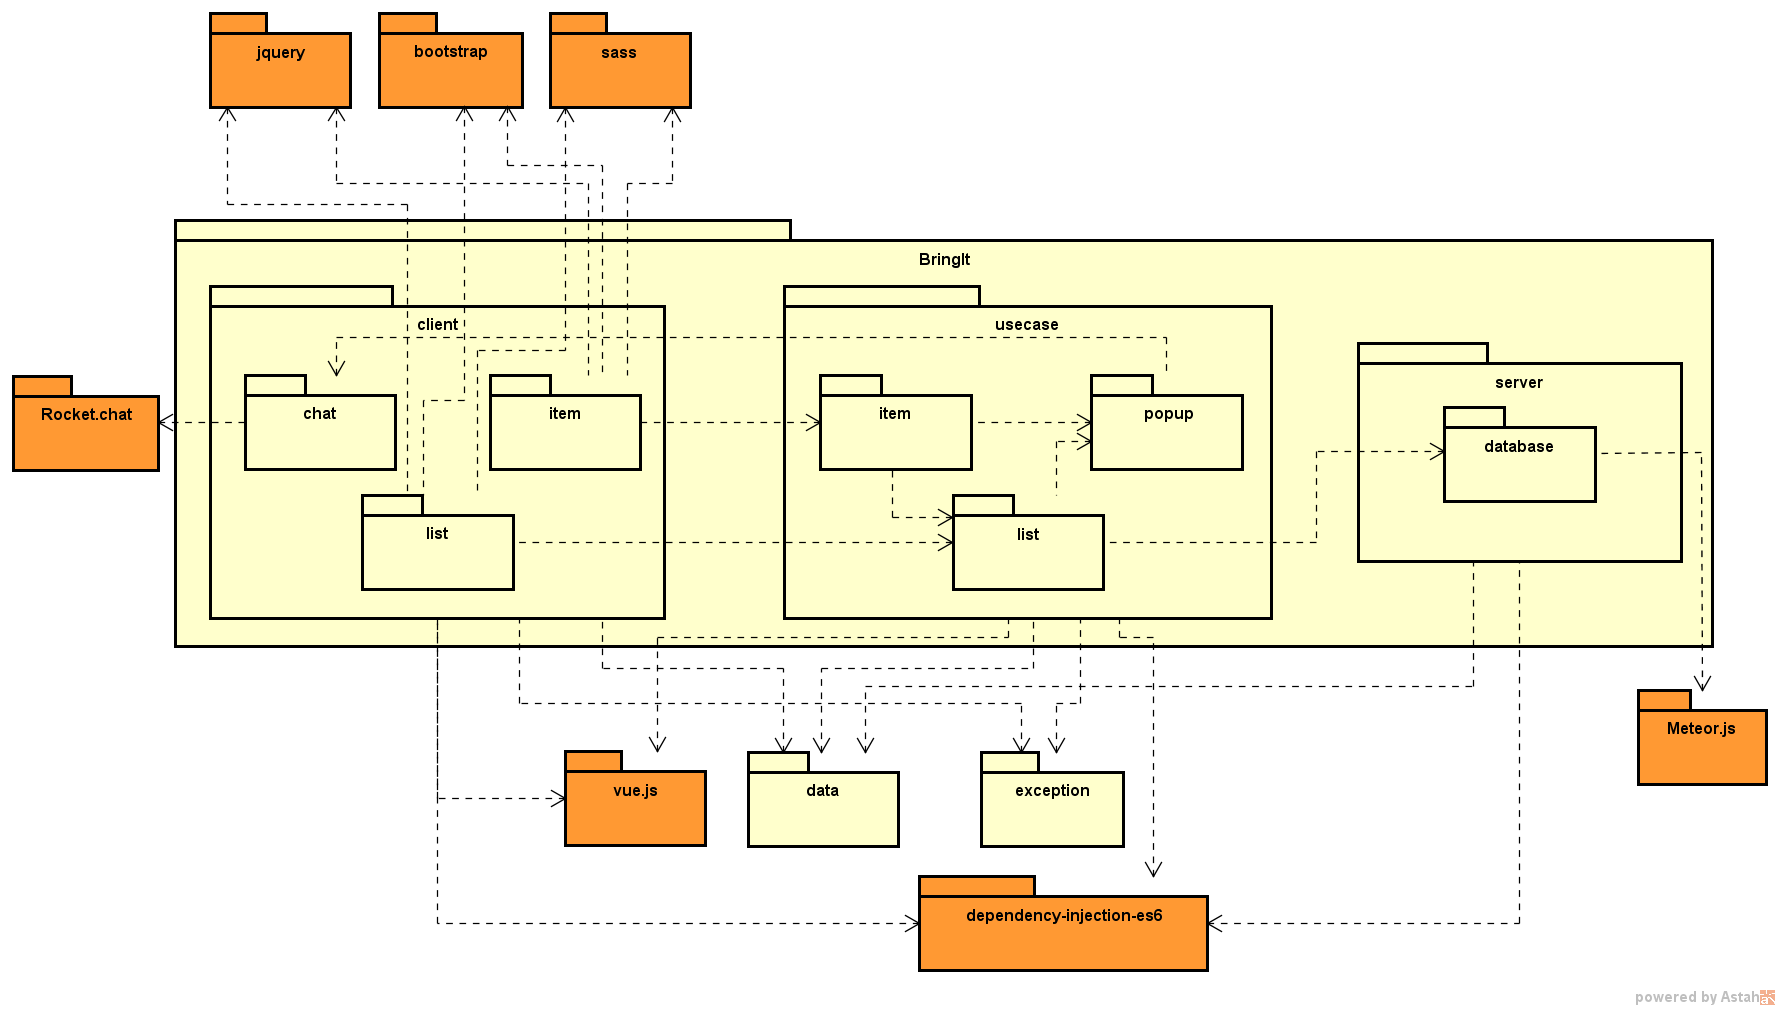
\includegraphics[scale=0.4]{Sezioni/Packages/App/pck_application.png}
%	\caption{Package application}
%\end{figure}


\subsection{SDK}

\subsubsection{Creazione di un widget immagine}

\label{Creazione di un widget immagine}
\begin{figure}[ht]
	\centering
	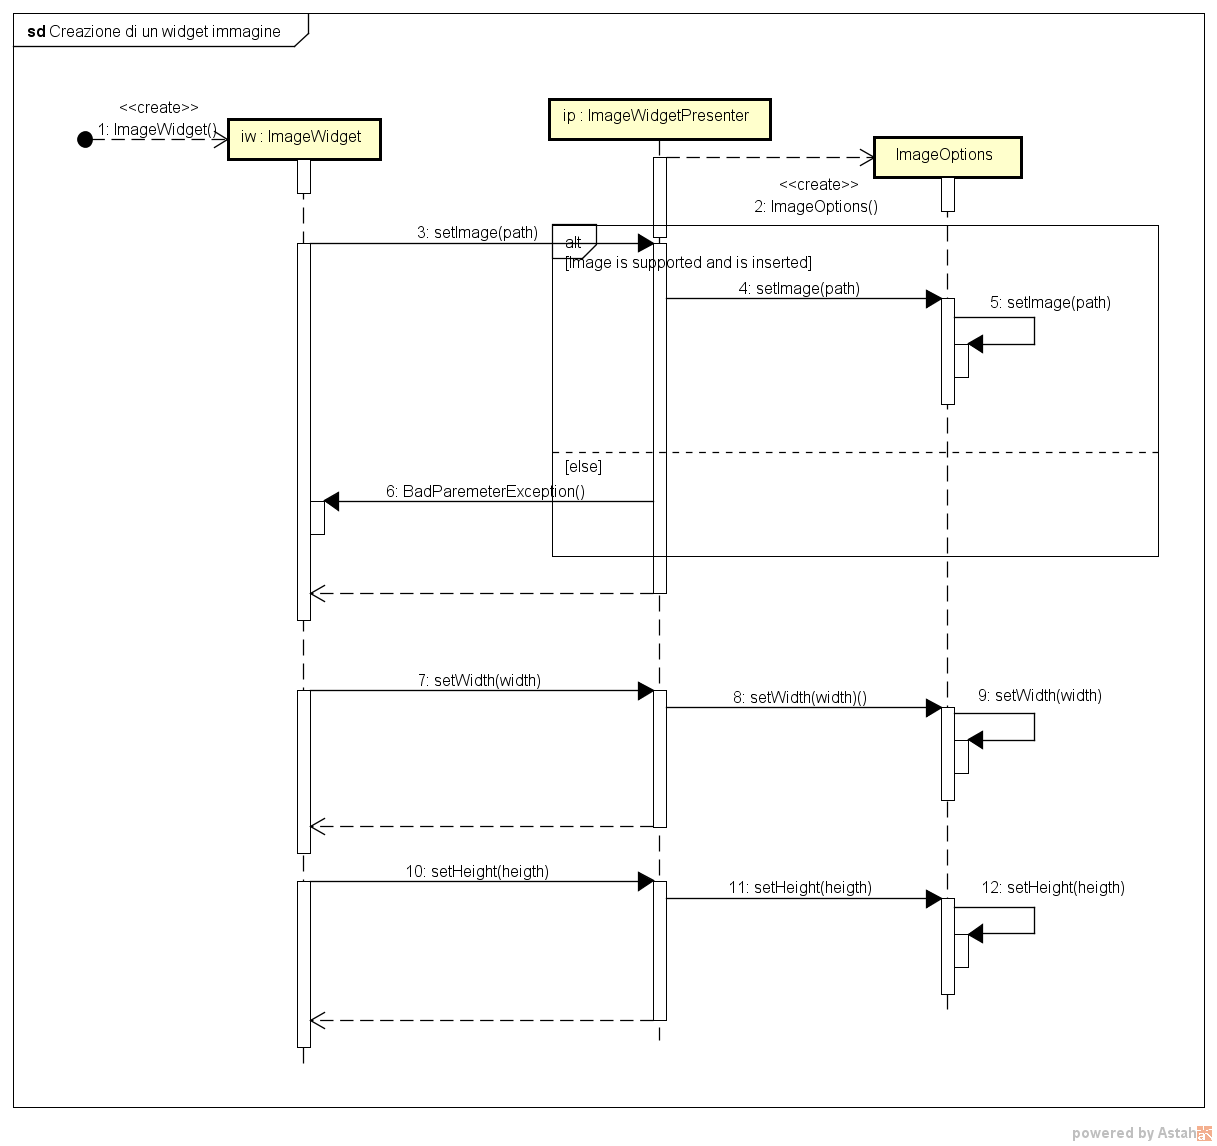
\includegraphics[width=16cm, height=14cm]{Sezioni/Diagrammi/img/Creazione di un widget immagine.png}
	\caption{Creazione di un widget immagine}
\end{figure}

Lo sviluppatore può creare un widget di tipo immagine per aggiungerlo ad una sua ipotetica \termine{bolla}. Durante la costruzione, come si vede dallo schema, vengono invocati tre metodi. Il primo per impostare l'immagine e gli altri due per impostare rispettivamente la larghezza ed altezza di essa. Il tipo delle immagini supportate sono le stesse supportate da \termine{Rocket.Chat} ovvero:
\begin{itemize}
\item .jpeg
\item .gif
\item .png
\item .jpg
\end{itemize}
Se l'immagine inserita non appartiene ad uno di questi formati oppure non viene inserita dallo sviluppatore il metodo \texttt{setText} di \texttt{TextWidgetPresenter} lancerà un'eccezione di tipo \texttt{BadParameterException}. \\
Le frecce di ritorno dall'\texttt{ImageWidgetPresenter} all'\texttt{ImageWidget} sono state inserite poiché il cambiamento dei dati sul \termine{Presenter} ha effetto anche sulla View. La comunicazione tra queste due unità avviene tramite il \termine{framework} \termine{vue.js}. \\
Si noti, infine, che i metodi invocati da \texttt{ImageWidget} vengono chiamati in quest'ordine dal suo costruttore senza parametri. Tali metodi possono anche essere chiamati singolarmente dallo sviluppatore secondo l'ordine che egli preferisce. Queste azioni non verranno ulteriormente descritte poiché ritenute ridondanti.

\newpage

\subsubsection{Creazione di un widget di testo}

\label{Creazione di un widget di testo}
\begin{figure}[H]
	\centering
	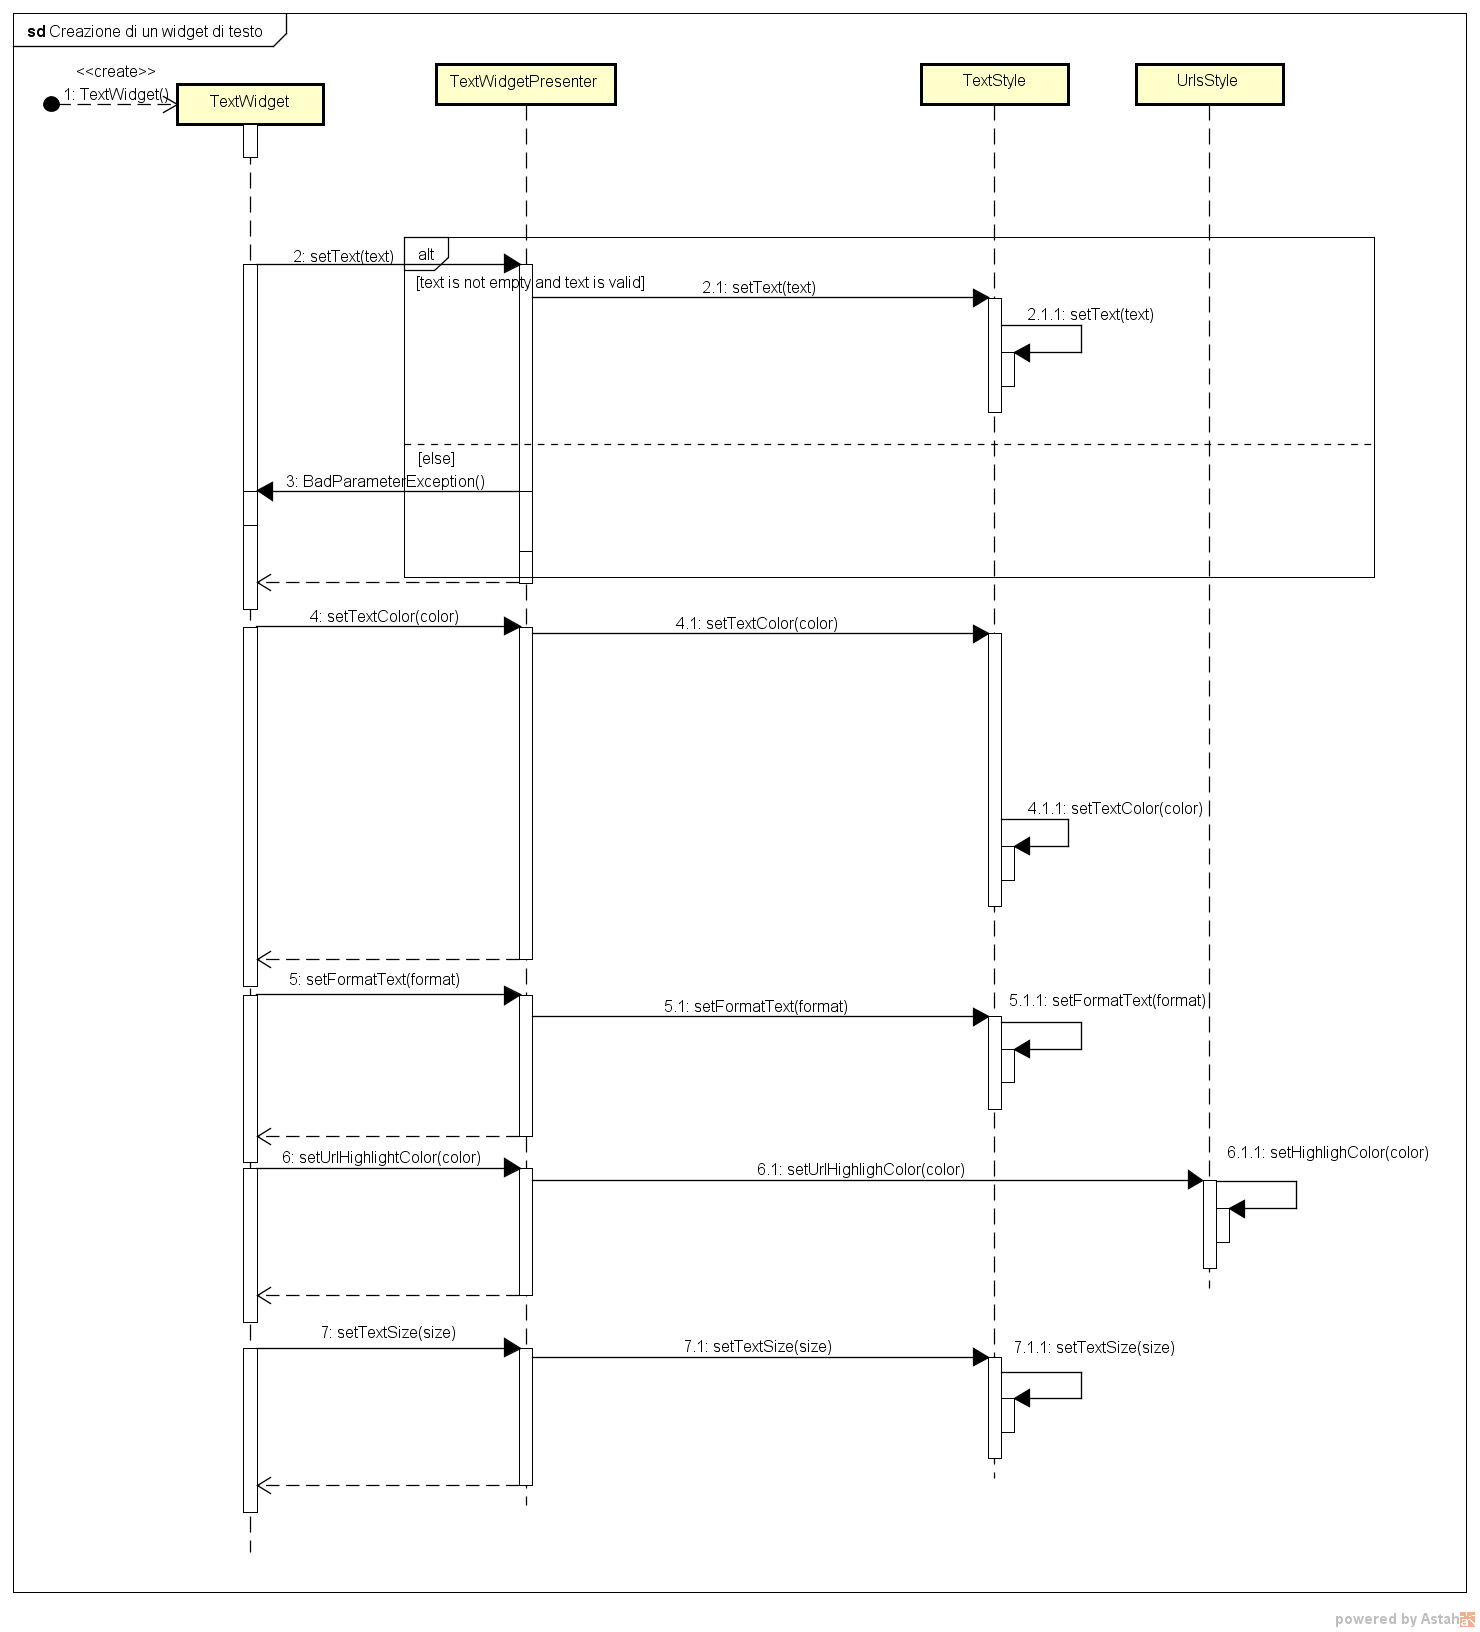
\includegraphics[width=16cm, height=14cm]{Sezioni/Diagrammi/img/Creazione di un widget di testo.png}
	\caption{Creazione di un widget di testo}
\end{figure}

Lo sviluppatore può creare un widget di tipo testo per aggiungerlo ad una sua ipotetica \termine{bolla}. Affinché non si verifichino errori il testo inserito nel widget deve essere valido, ovvero non deve contenere caratteri speciali se non quelli supportati dal tipo di codifica UTF-8 e non deve essere del testo vuoto. Se ciò dovesse capitare il metodo \texttt{setText} di \texttt{TextWidgetPresenter} lancerà un'eccezione di tipo \texttt{BadParameterException}. \\
Le frecce di ritorno dal \texttt{TextWidgetPresenter}  al \texttt{TextWidget} sono state inserite poiché il cambiamento dei dati sul \termine{Presenter} ha effetto anche sulla View. La comunicazione tra queste due unità avviene tramite il \termine{framework} \termine{vue.js}. \\
Si noti, infine, che i metodi invocati da \texttt{TextWidget} vengono chiamati in quest'ordine dal suo costruttore senza parametri. Tali metodi possono anche essere chiamati singolarmente dallo sviluppatore secondo l'ordine che egli preferisce. Queste azioni non verranno ulteriormente descritte poiché ritenute ridondanti.

\newpage

\subsubsection{Creazione di un widget Checklist}

\label{Creazione di un widget Checklist}
\begin{figure}[H]
	\centering
	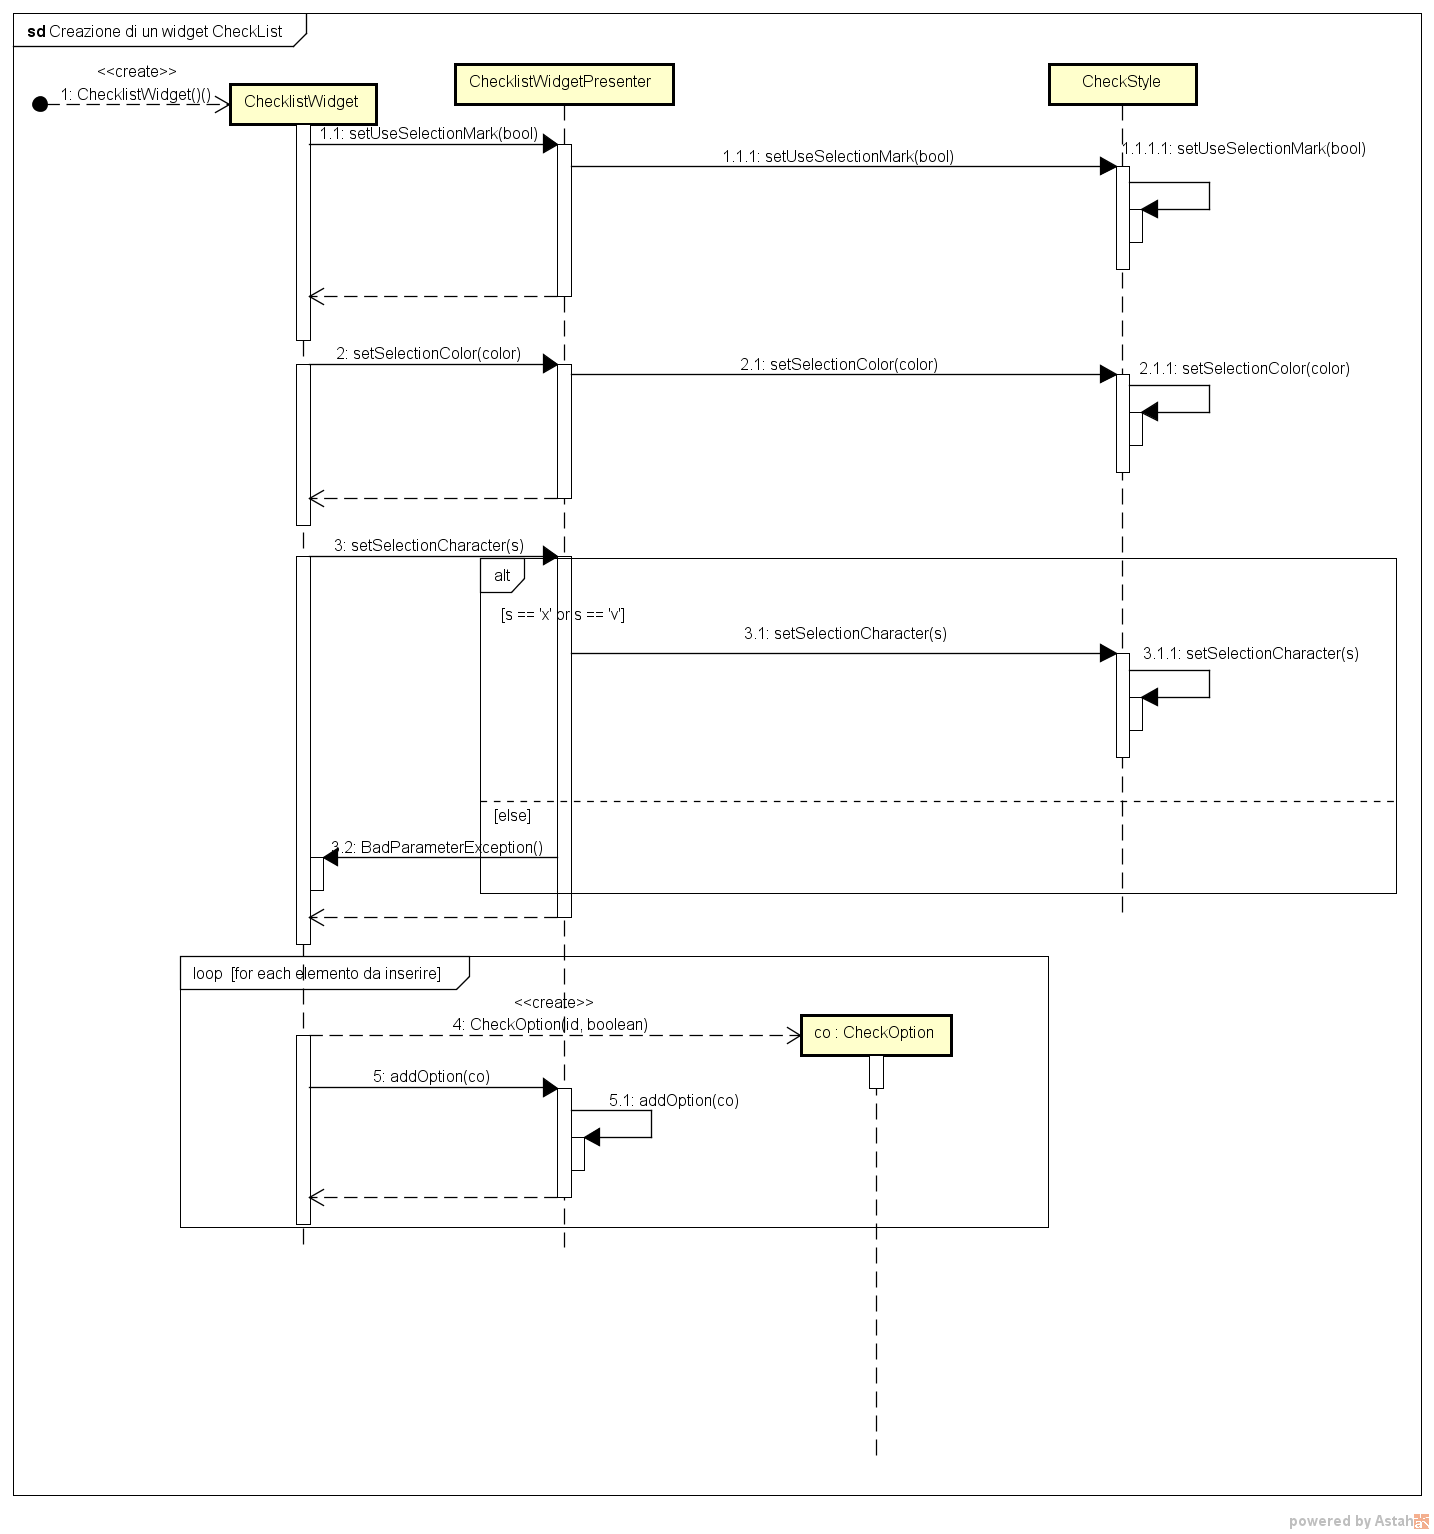
\includegraphics[width=16cm, height=14cm]{Sezioni/Diagrammi/img/Creazione di un widget CheckList.png}
	\caption{Creazione di un widget Checklist}
\end{figure}

Lo sviluppatore può creare un widget di tipo Checklist per aggiungerlo ad una sua ipotetica \termine{bolla}. Affinché non si verifichino errori, quando si usa il metodo \texttt{setSelectionCharacter} deve essere inserito correttamente un carattere per la spunta supportato. Inoltre se il flag \texttt{useSelectionMark} è stato impostato a false allora, indipendentemente dal carattere scelto dalla spunta, verrà usato il colore.\\
Le frecce di ritorno dal \texttt{ChecklistWidgetPresenter}  al \texttt{ChecklistWidget} sono state inserite poiché il cambiamento dei dati sul \termine{Presenter} ha effetto anche sulla View. La comunicazione tra queste due unità avviene tramite il \termine{framework} \termine{vue.js}. \\
Si noti, infine, che i metodi invocati da \texttt{Checklist} vengono chiamati in quest'ordine dal suo costruttore senza parametri. Tali metodi possono anche essere chiamati singolarmente dallo sviluppatore secondo l'ordine che egli preferisce. Queste azioni non verranno ulteriormente descritte poiché ritenute ridondanti.

\newpage

\subsubsection{Aggiungere un messaggio di completamento al widget Checklist}

\label{Aggiungere un messaggio di completamento al widget Checklist}
\begin{figure}[H]
	\centering
	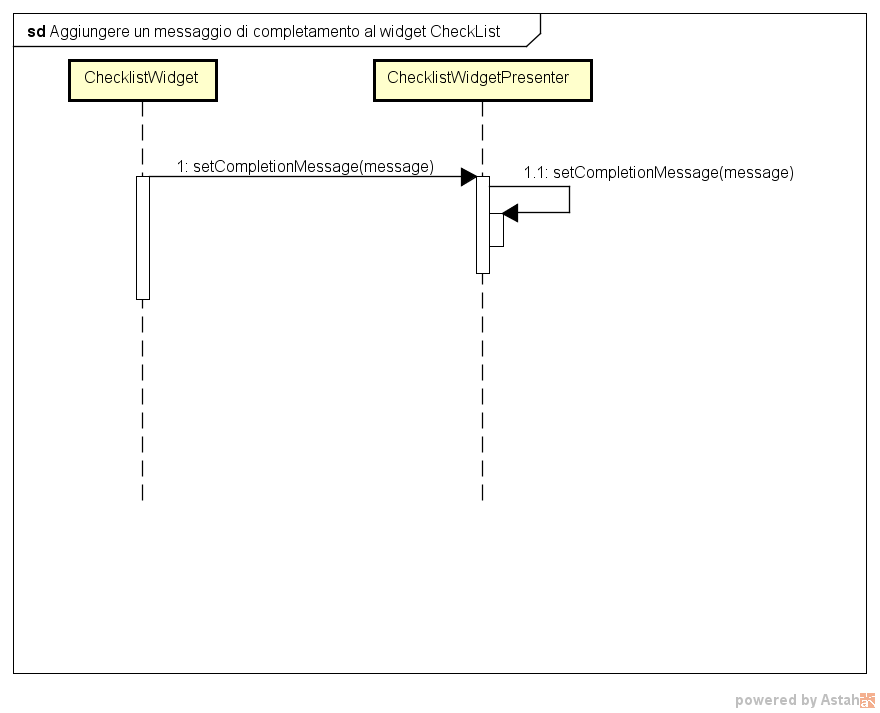
\includegraphics[width=16cm, height=14cm]{Sezioni/Diagrammi/img/Aggiungere un messaggio di completamento al widget Checklist.png}
	\caption{Aggiungere un messaggio di completamento al widget Checklist}
\end{figure}

Lo sviluppatore può aggiungere un messaggio di completamento per il widget Checklist. Questo messaggio verrà visualizzato non appena tutte le entry del widget saranno spuntate, ovvero al lancio dell'evento \texttt{emitOnCompletedList}.

\newpage

\subsubsection{Creazione di un widget bottone}

\label{Creazione di un widget bottone}
\begin{figure}[H]
	\centering
	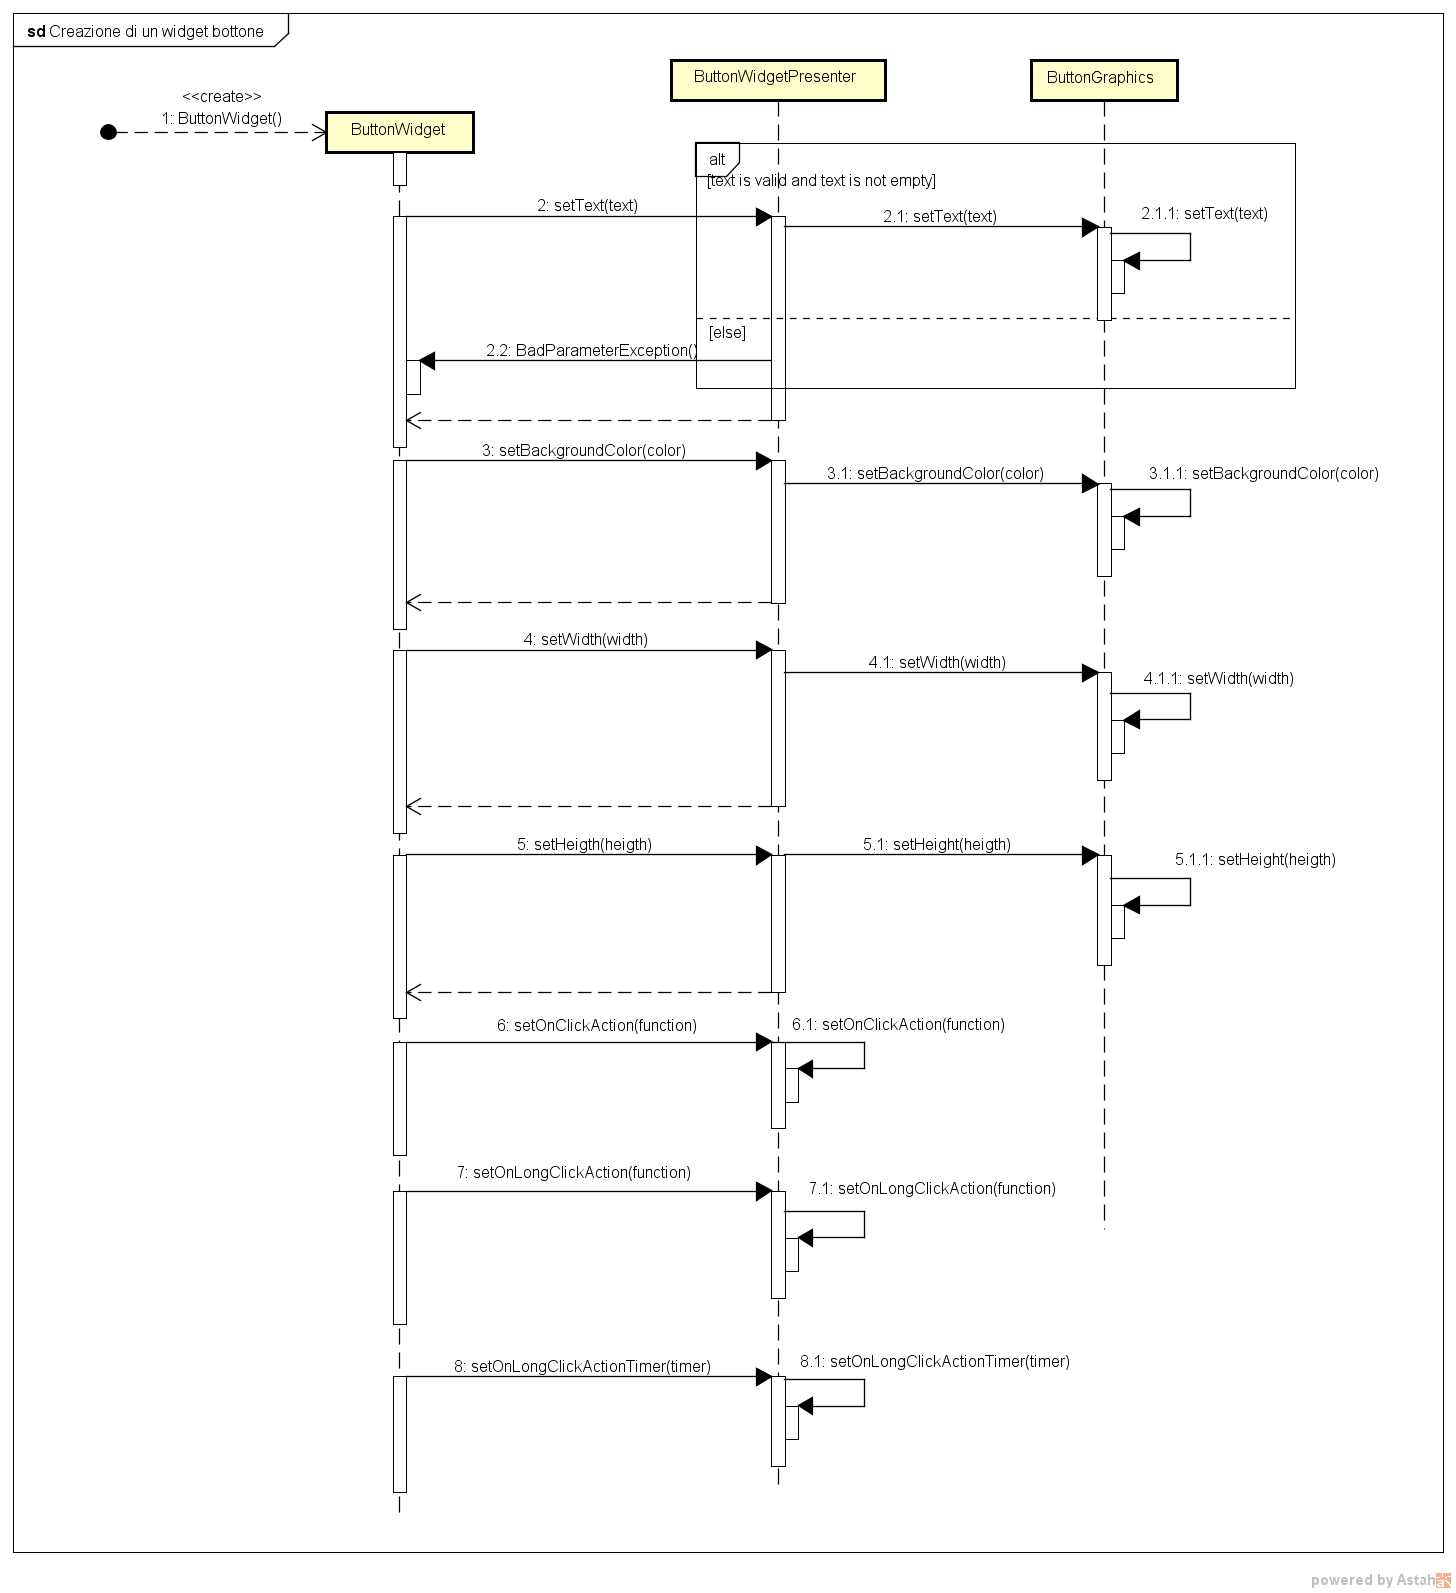
\includegraphics[width=16cm, height=14cm]{Sezioni/Diagrammi/img/Creazione di un widget bottone.png}
	\caption{Creazione di un widget bottone}
\end{figure}

Lo sviluppatore può creare un widget di tipo bottone per aggiungerlo ad una sua ipotetica \termine{bolla}. Se, durante la creazione del widget, il testo non dovesse essere impostato correttamente, il metodo \texttt{setText} di \texttt{ButtonWidgetPresenter} lancerà un'eccezione di tipo \texttt{BadParameterException}. \\
Le frecce di ritorno da \texttt{ButtonWidgetPresenter}  a \texttt{ButtonWidget} sono state inserite poiché il cambiamento dei dati sul \termine{Presenter} ha effetto anche sulla View. La comunicazione tra queste due unità avviene tramite il \termine{framework} \termine{vue.js}. \\
Si noti, infine, che i metodi invocati da \texttt{ButtonWidget} vengono chiamati in quest'ordine dal suo costruttore senza parametri. Tali metodi possono anche essere chiamati singolarmente dallo sviluppatore secondo l'ordine che egli preferisce. Queste azioni non verranno ulteriormente descritte poiché ritenute ridondanti.

\newpage

\subsubsection{Creazione di un listWidget}

\label{Click di un bottone}
\begin{figure}[H]
	\centering
	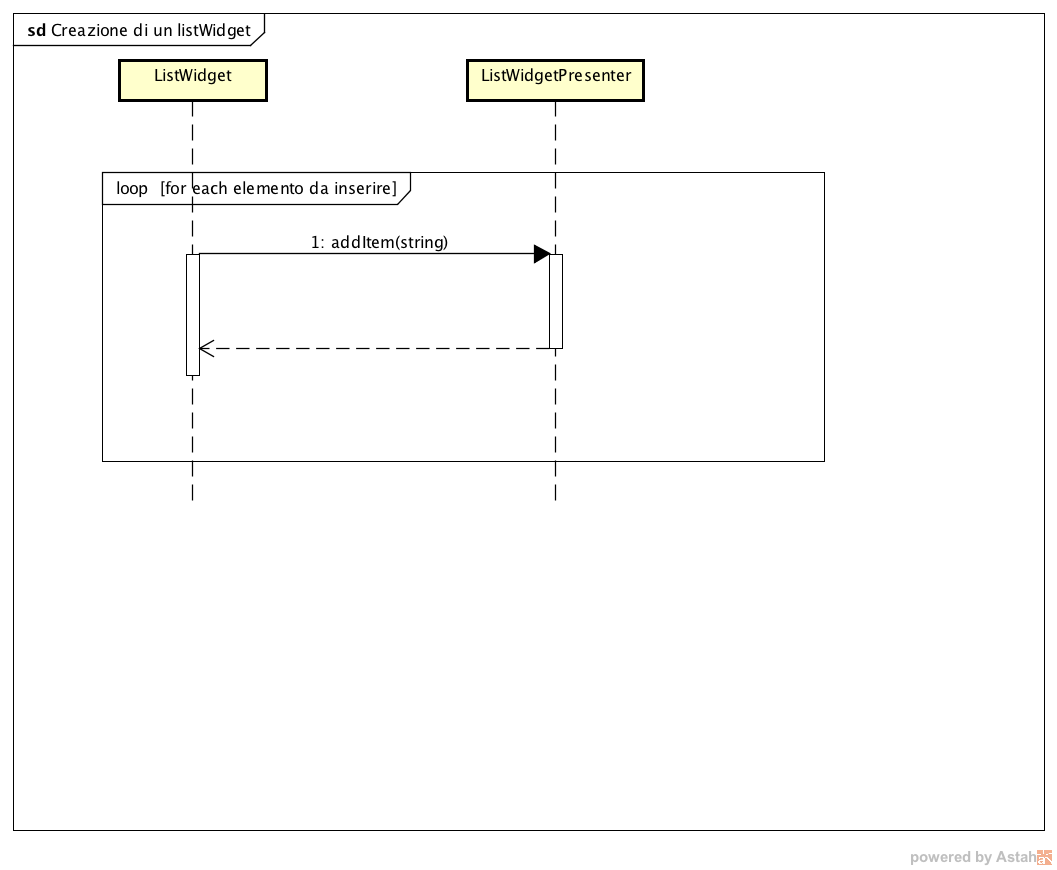
\includegraphics[width=16cm, height=14cm]{Sezioni/Diagrammi/img/Creazione di un listWidget.png}
	\caption{Creazione di un listWidget}
\end{figure}

Lo sviluppatore può creare un widget di tipo lista per aggiungerlo ad una sua ipotetica \termine{bolla}. Ogni elemento aggiunto logicamente dal presenter agisce anche sulla view. Per questo tipo di comunicazione si rimanda al \termine{framework} \termine{vue.js}. \\
L'azione compiuta per creare il widget può essere anche effettuata a posteriori della creazione del widget, questa però, essendo molto simile a quella appena descritta, viene omessa per ridondanza.

\newpage

\subsubsection{Creazione di una bolla aggiungendo un widget checklist}

\label{Creazione di una bolla aggiungendo un widget checklist}
\begin{figure}[H]
	\centering
	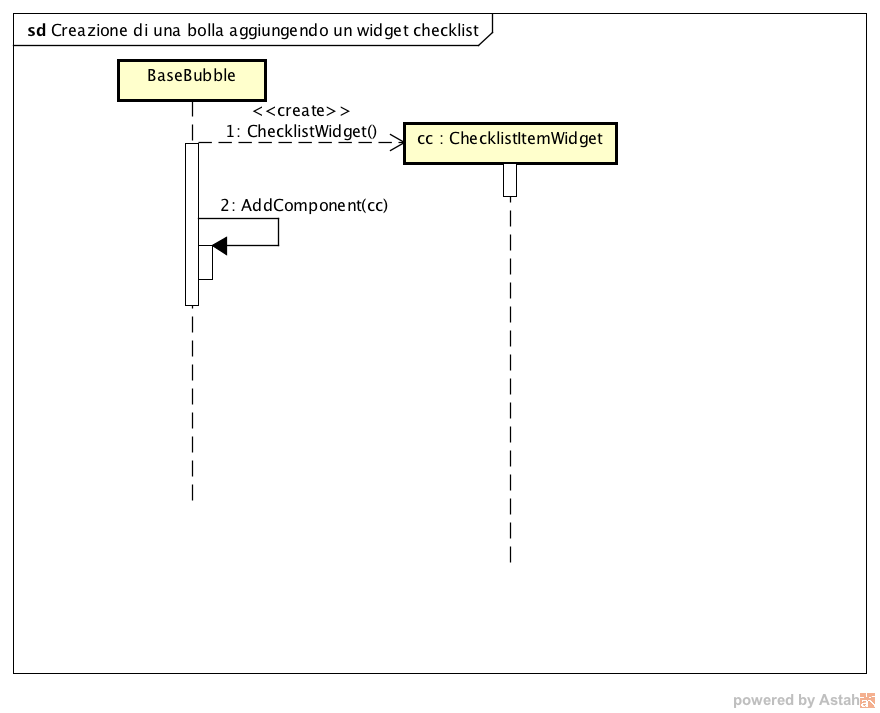
\includegraphics[width=16cm, height=14cm]{Sezioni/Diagrammi/img/Creazione di una bolla aggiungendo un widget checklist.png}
	\caption{Creazione di una bolla aggiungendo un widget checklist}
\end{figure}

Lo sviluppatore può aggiungere un widget alla \termine{bolla} appena creata. L'aggiunta dell'elemento avviene tramite il metodo \texttt{addComponent} che permette l'aggiunta sia di un layout che di un widget. Si noti che l'esempio è fatto con un widget specifico, ovvero il widget checklist, ma ciò vale per qualsiasi widget presente nell'\termine{SDK}. Gli altri esempi simili vengono, per questo motivo, omessi.

\newpage

\subsubsection{Aggiunta ad una bolla di un Layout contenente due widget di testo}

\label{Aggiunta ad una bolla di un Layout contenente due widget di testo}
\begin{figure}[H]
	\centering
	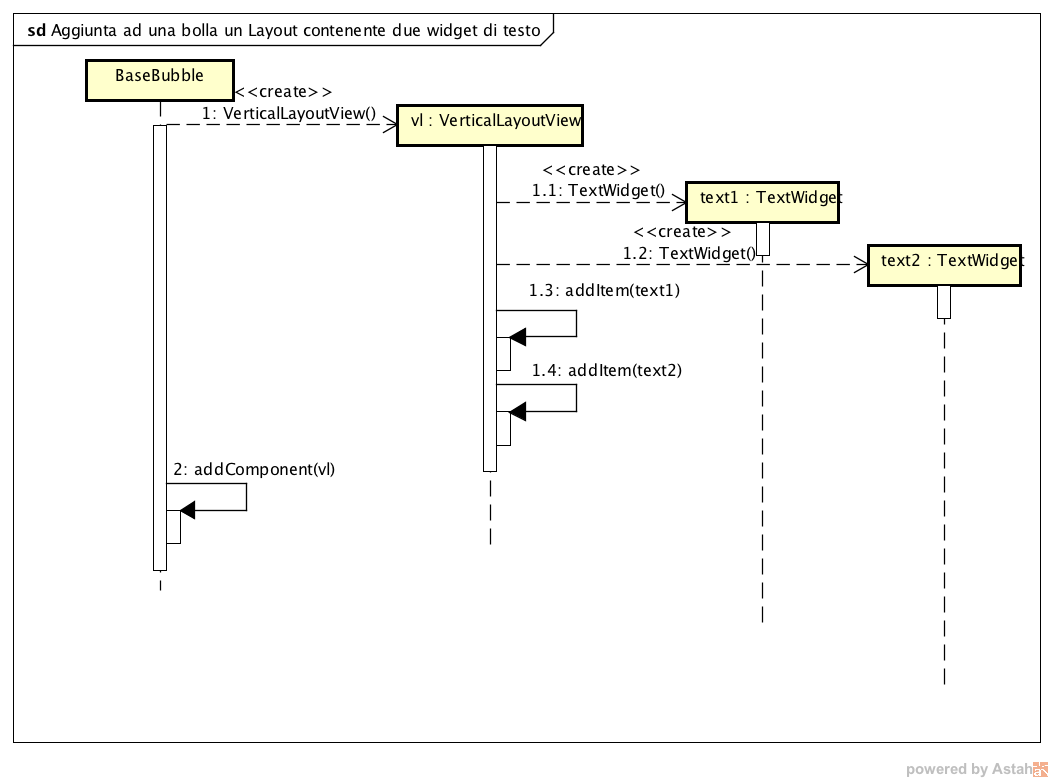
\includegraphics[width=16cm, height=14cm]{Sezioni/Diagrammi/img/Aggiunta ad una bolla un Layout contenente due widget di testo.png}
	\caption{Aggiunta ad una bolla di un Layout contenente due widget di testo}
	
\end{figure}
Lo sviluppatore può aggiungere un layout contenente dei widgets alla \termine{bolla}. Anche questo rappresenta solo un generico esempio di come si possa aggiungere un layout ad una \termine{bolla}. Gli altri esempi simili saranno dunque omessi. 

\newpage

\subsubsection{Creazione di una bolla MarkDownBubble}

\label{Creazione di una bolla MarkDownBubble}
\begin{figure}[H]
	\centering
	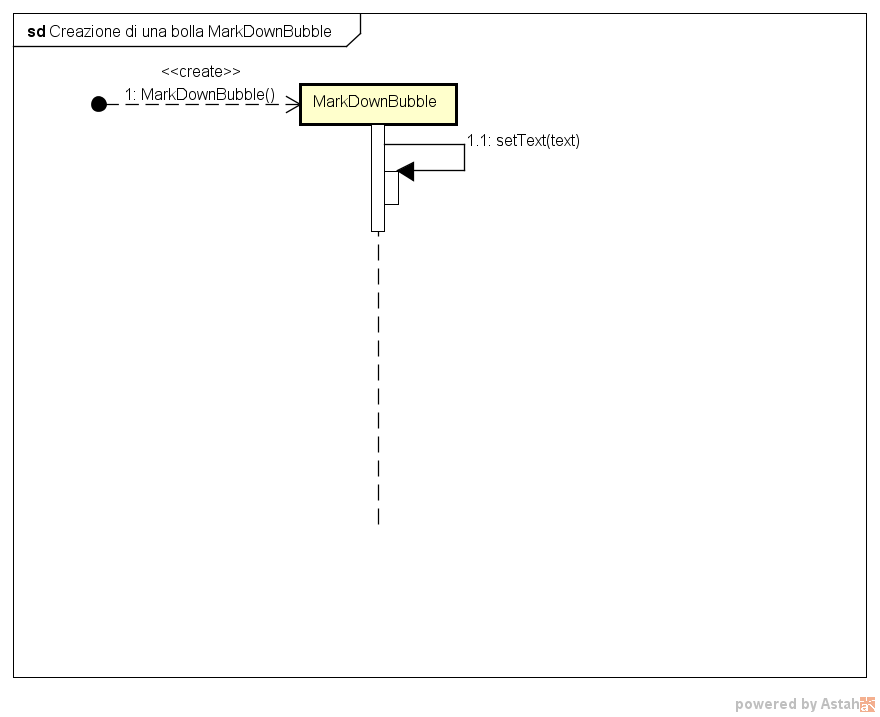
\includegraphics[width=12cm, height=8cm]{Sezioni/Diagrammi/img/Creazione di una bolla MarkDownBubble.png}
	\caption{Creazione di una bolla MarkDownBubble}
	
\end{figure}

Lo sviluppatore può creare una \termine{bolla} MarkDownBubble disponibile nell'\termine{SDK}.

\subsubsection{Creazione di una bolla AlertBubble}

\label{Creazione di una bolla AlertBubble}
\begin{figure}[H]
	\centering
	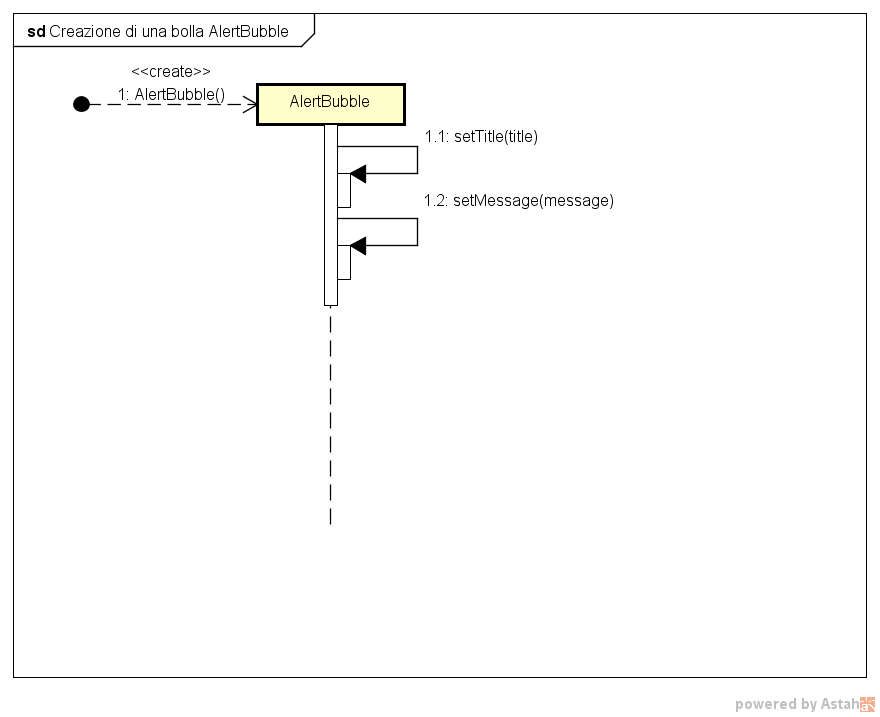
\includegraphics[width=12cm, height=8cm]{Sezioni/Diagrammi/img/Creazione di una bolla AlertBubble.png}
	\caption{Creazione di una bolla AlertBubble}
	
\end{figure}

Lo sviluppatore può creare una \termine{bolla} AlertBubble disponibile nell'\termine{SDK}.

\newpage

\subsubsection{Creazione di una bolla ToDoListBubble}

\label{Creazione di una bolla ToDoListBubble}
\begin{figure}[H]
	\centering
	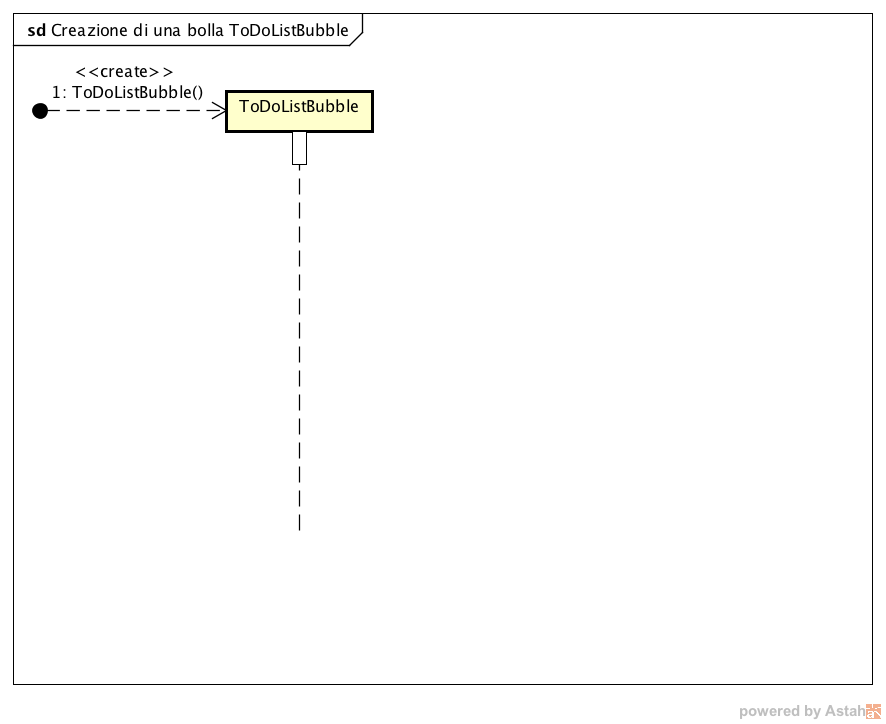
\includegraphics[width=12cm, height=8cm]{Sezioni/Diagrammi/img/Creazione di una bolla ToDoListBubble.png}
	\caption{Creazione di una bolla ToDoListBubble}
	
\end{figure}

Lo sviluppatore può creare una \termine{bolla} ToDoListBubble disponibile nell'\termine{SDK}.



\subsection{Package application}
\label{Package application}
\begin{figure}[H]
	\centering
	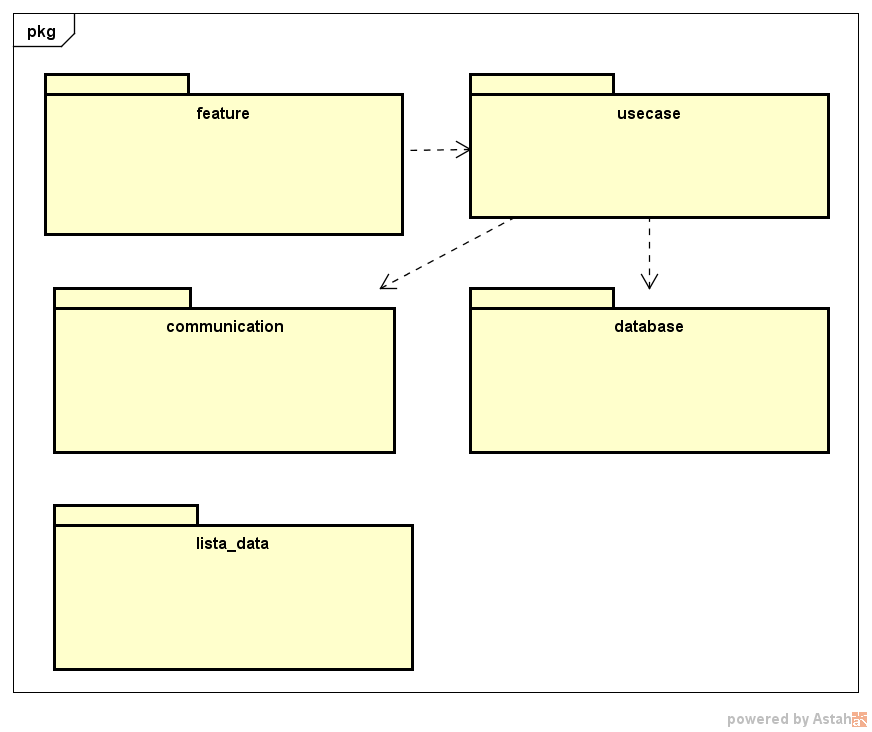
\includegraphics[scale=0.5]{Sezioni/Packages/App/application.png}
	\caption{Package application}
\end{figure}
\begin{itemize}
	\item \textbf{Descrizione}: \termine{Package} contenente tutti i file dell'applicazione demo.
	\item \textbf{Classi e packages contenuti}:
	\begin{itemize}
		\item application::feature: package contenente tutte le feature principali dell'applicazione
		\item application::usecase: package contenente tutti gli usecase dell'applicazione
		\item application::lista\_data: package contenente le classi che modellano i dati dell'applicazione
		\item application::database: package contenente tutte le classi relative ai database
	\end{itemize}
	\item application::communication: package contenente tutte le classi atte a comunicare con la chat
\end{itemize}


\subsubsection{Package application::usecase}
\label{Package application::usecase}
\begin{figure}[H]
	\centering
	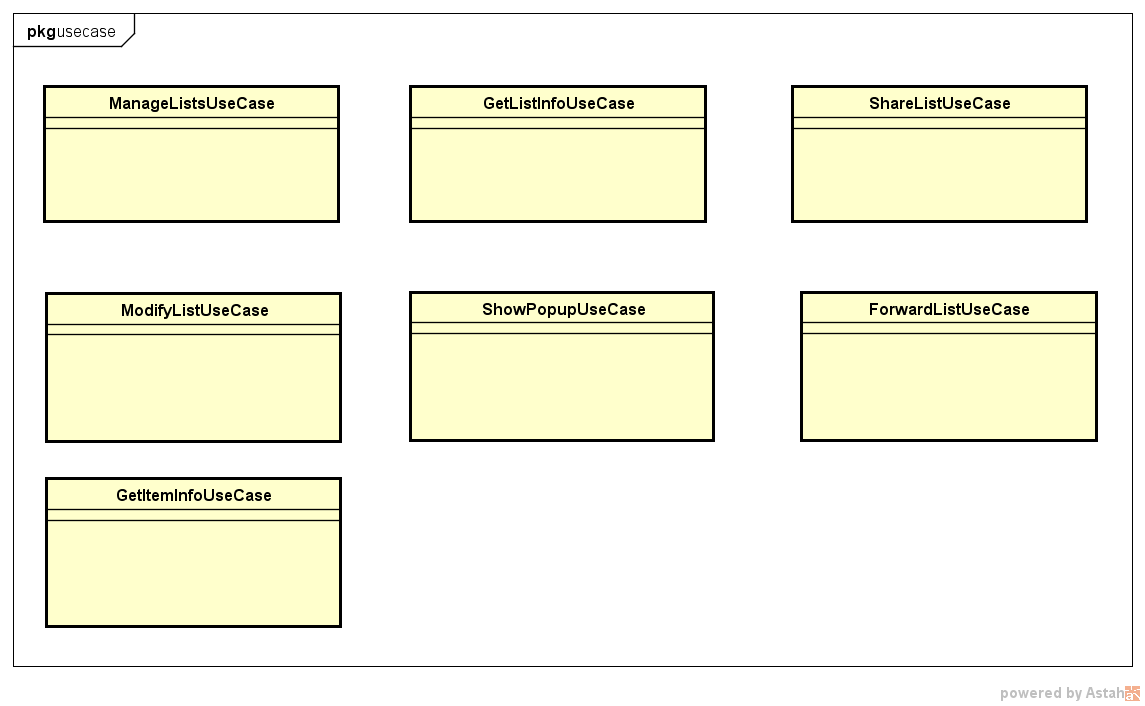
\includegraphics[scale=0.5]{Sezioni/Packages/App/usecase.png}
	\caption{Package application::usecase}
\end{figure}
\begin{itemize}
	\item \textbf{Descrizione}: package contenente tutte le classi che gestiscono la logica dell'applicazione
	\item \textbf{Classi e packages contenuti}:
	\begin{itemize}
	\item application::usecase::ManageListsUseCase: classe che gestisce le modifiche alle liste memorizzate nel database
	\item application::usecase GetListInfoUseCase: classe che recupera i dati di una lista dal database
	\item application::usecase:ModifyListUseCase: classe che permette la modifica di una lista memorizzata all'interno del database
	\item application::usecase ShowPopupUseCase: classe che permette la visualizzazione di finestre modali
	\item application::usecase::GetItemInfoUseCase: classe che permette di recuperare le informazioni di un particolare oggetto in una lista dal database
	\end{itemize}
\end{itemize}

\subsubsection{Package application::lista\_data}
\label{Package application::lista_data}
\begin{figure}[H]
	\centering
	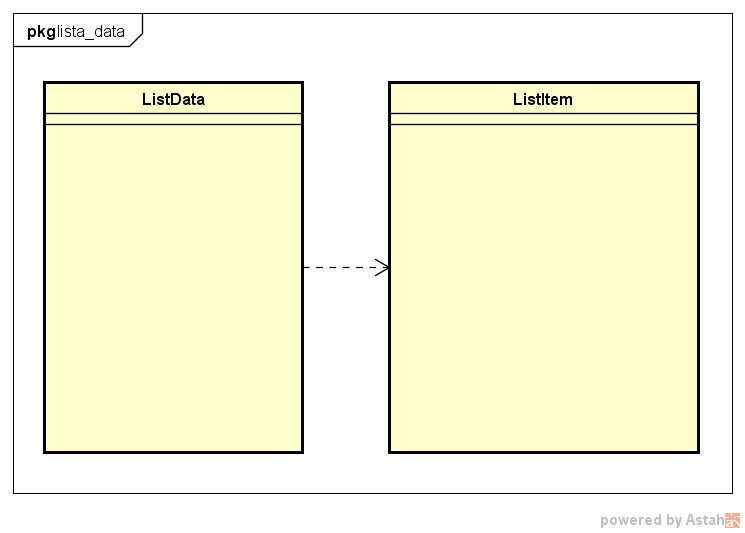
\includegraphics[scale=0.5]{Sezioni/Packages/App/lista_data.png}
	\caption{Package application::lista\_data}
\end{figure}
\begin{itemize}
	\item \textbf{Descrizione}: package contenente tutte le classi che modellano gli oggetti di una lista e di un oggetti di una lista
	\item \textbf{Classi e packages contenuti}:
	\begin{itemize}
	\item application::lista\_data::ListData: classe che modella una lista
	\item application::lista\_data::ListItem: classe che modella un oggetto di una lista
	\end{itemize}
\end{itemize}

\subsubsection{Package application::communication}
\label{Package application::communication}
\begin{figure}[H]
	\centering
	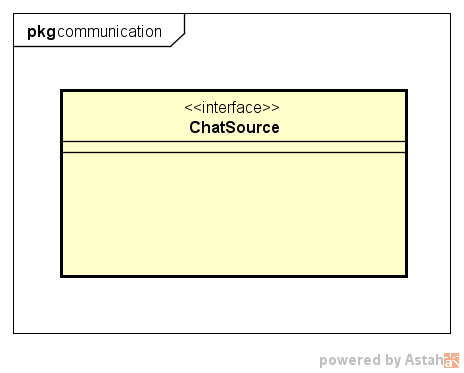
\includegraphics[scale=0.5]{Sezioni/Packages/App/communication.png}
	\caption{Package application::communication}
\end{figure}
\begin{itemize}
	\item \textbf{Descrizione}: package che contiene le classi di comunicazione con l'istanza di Rocket.chat
	\item \textbf{Classi e packages contenuti}:
	\begin{itemize}
	\item application::communication::ChatSource: interfaccia che permette la comunicazione con l'istanza di Rocket.chat
	\end{itemize}
\end{itemize}

\subsubsection{Package application::database}
\label{Package application::database}
\begin{figure}[H]
	\centering
	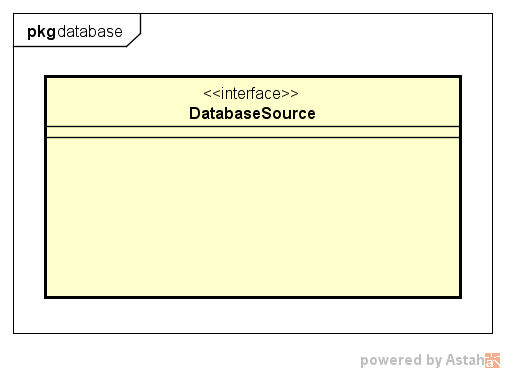
\includegraphics[scale=0.5]{Sezioni/Packages/App/database.png}
	\caption{Package application::database}
\end{figure}
\begin{itemize}
	\item \textbf{Descrizione}: package che contiene le classi per interfacciarsi con il database all'interno del quale sono salvati i dati delle liste
	\item \textbf{Classi e packages contenuti}:
	\begin{itemize}
	\item application::database::DatabaseSource: interfaccia che permette la comunicazione con il database all'interno del quale sono salvati i dati delle varie liste
	\end{itemize}
\end{itemize}

\subsubsection{Package application::feature::add\_item}
\label{Package application::feature::add_item}
\begin{figure}[H]
	\centering
	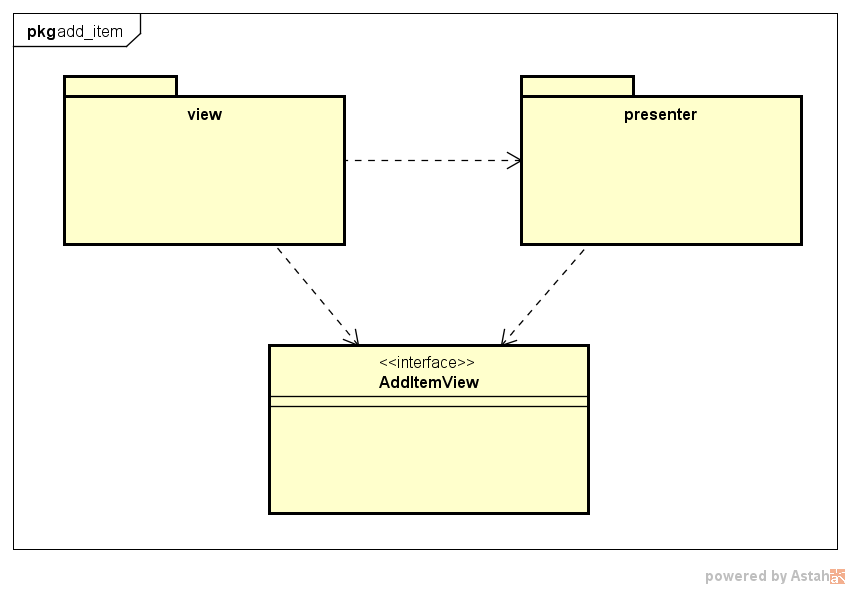
\includegraphics[scale=0.5]{Sezioni/Packages/App/add_item.png}
	\caption{Package application::feature::add\_item}
\end{figure}
\begin{itemize}
	\item \textbf{Descrizione}: package contenente i file relativi alla funzionalità di aggiunta elemento ad una lista
	\item \textbf{Classi e packages contenuti}:
	\begin{itemize}
	\item application::feature::add\_item::view: package contenente la view per l'aggiunta di un elemento
	\item application::feature::add\_item::presenter: package contenente il presenter per la view di aggiunta elemento
	\item application::feature::add\_item::AddItemView: interfaccia che rappresenta la vista di aggiunta oggetto
	\end{itemize}
\end{itemize}

\subsubsection{Package application::feature::add\_item::view}
\label{Package application::feature::add_item::view}
\begin{figure}[H]
	\centering
	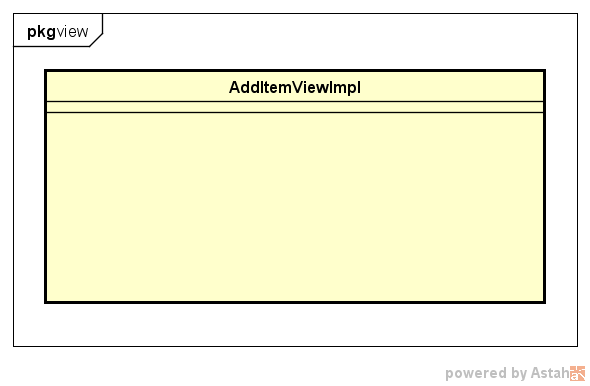
\includegraphics[scale=0.5]{Sezioni/Packages/App/add_item_view.png}
	\caption{Package application::feature::add\_item::view}
\end{figure}
\begin{itemize}
	\item \textbf{Descrizione}: package contenente la view per l'aggiunta di un elemento
	\item \textbf{Classi e packages contenuti}:
	\begin{itemize}
	\item application::feature::add\_item::view::AddItemViewImpl: implementazione dell'interfaccia AddItemView che rappresenta la vista di aggiunta di un oggetto alla lista
	\end{itemize}
\end{itemize}

\subsubsection{Package application::feature::add\_item::presenter}
\label{Package application::feature::add_item::presenter}
\begin{figure}[H]
	\centering
	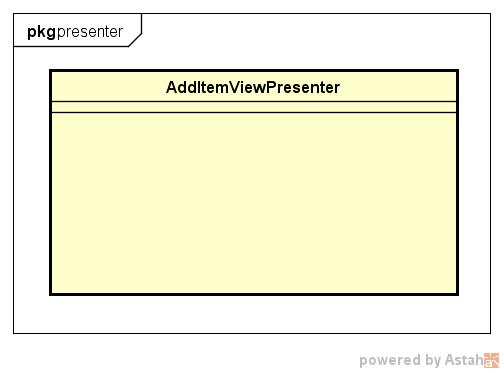
\includegraphics[scale=0.5]{Sezioni/Packages/App/add_item_presenter.png}
	\caption{Package application::feature::add\_item::presenter}
\end{figure}
\begin{itemize}
	\item \textbf{Descrizione}: package contenente il presenter per la vista di aggiunta di un oggetto alla lista
	\item \textbf{Classi e packages contenuti}:
	\begin{itemize}
	\item application::feature::add\_item::presenter::AddItemViewPresenter: presenter per la vista di aggiunta di un oggetto alla lista
	\end{itemize}
\end{itemize}

\subsubsection{Package application::feature::change\_list\_info}
\label{Package application::feature::change_list_info}
\begin{figure}[H]
	\centering
	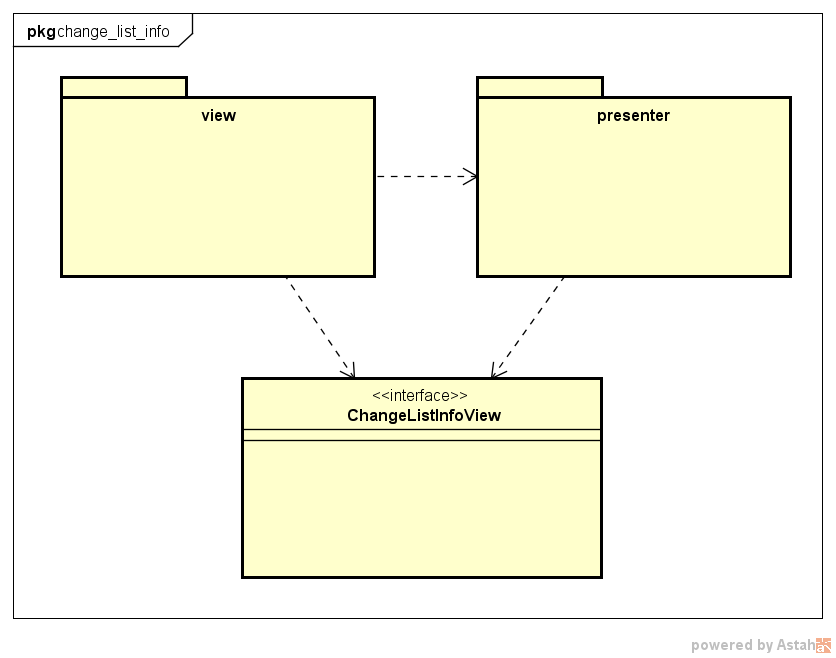
\includegraphics[scale=0.5]{Sezioni/Packages/App/change_list_info.png}
	\caption{Package application::feature::change\_list\_info}
\end{figure}
\begin{itemize}
	\item \textbf{Descrizione}: package contenente i componenti per la funzionalità di modifica informazioni di una lista
	\item \textbf{Classi e packages contenuti}:
	\begin{itemize}
	\item application::feature::change\_list\_info::view: package contenente la vista per la modifica informazioni di una lista
	\item application::feature::change\_list\_info::presenter: package contenente il presenter per la vista di modifica informazioni di una lista
	\item application::feature::change\_list\_info::ChangeListInfoView: interfaccia rappresentante la vista per la modifica informazioni di una lista
	\end{itemize}
\end{itemize}

\subsubsection{Package application::feature::change\_list\_info::view}
\label{Package application::feature::change_list_info::view}
\begin{figure}[H]
	\centering
	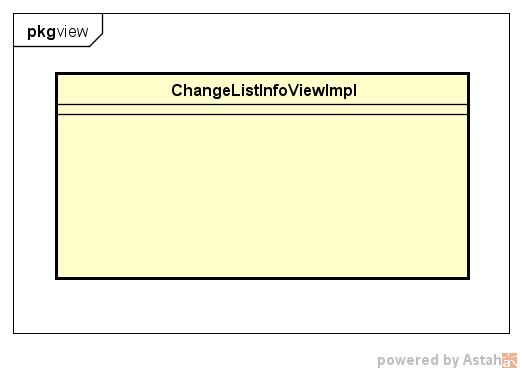
\includegraphics[scale=0.5]{Sezioni/Packages/App/change_list_info_view.png}
	\caption{Package application::feature::change\_list\_info::view}
\end{figure}
\begin{itemize}
	\item \textbf{Descrizione}: package contenente la vista per la funzionalità di modifica informazioni di una lista
	\item \textbf{Classi e packages contenuti}:
	\begin{itemize}
	\item application::feature::change\_list\_info::view::ChangeListInfoViewImpl: implementazione dell'interfaccia che rappresenta la vista per la funzionalità di modifica della informazioni di una lista
	\end{itemize}
\end{itemize}

\subsubsection{Package application::feature::change\_list\_info::presenter}
\label{Package application::feature::change_list_info::presenter}
\begin{figure}[H]
	\centering
	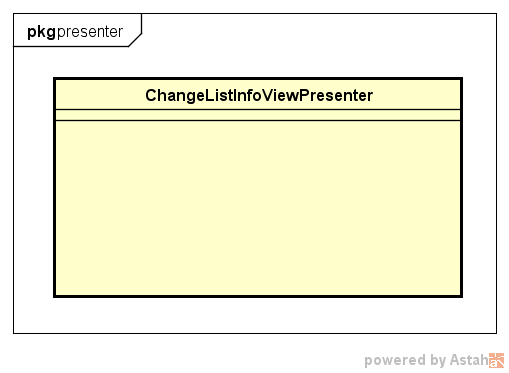
\includegraphics[scale=0.5]{Sezioni/Packages/App/change_list_info_presenter.png}
	\caption{Package application::feature::change\_list\_info::presenter}
\end{figure}
\begin{itemize}
	\item \textbf{Descrizione}: package contenente il presenter per la vista di modifica informazioni di una lista
	\item \textbf{Classi e packages contenuti}:
	\begin{itemize}
	\item application::feature::change\_list\_info::presenter::ChangeListInfoViewPresenter: classe che rappresenta il presenter per la vista di modifica dei dati di una lista
	\end{itemize}
\end{itemize}


\subsubsection{Package application::feature::create\_list}
\label{Package application::feature::create_list}
\begin{figure}[H]
	\centering
	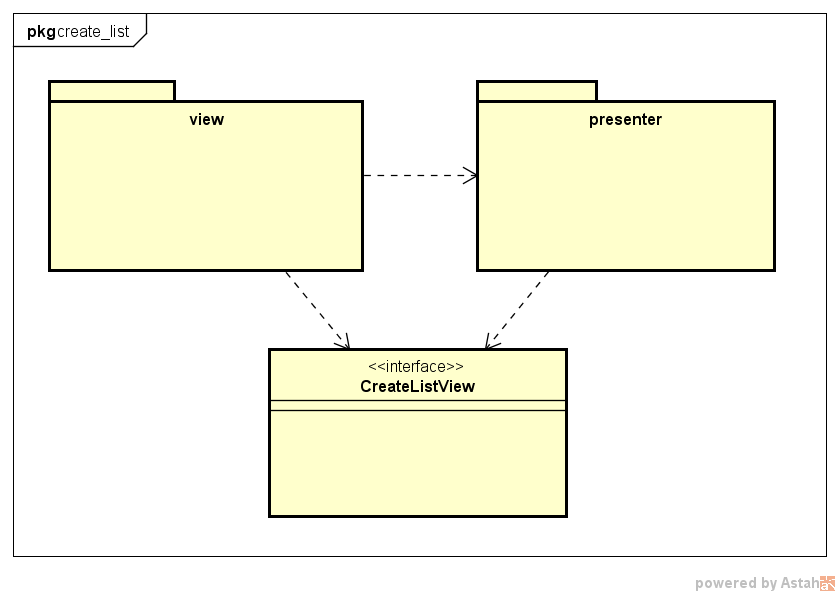
\includegraphics[scale=0.5]{Sezioni/Packages/App/create_list.png}
	\caption{Package application::feature::create\_list}
\end{figure}
\begin{itemize}
	\item \textbf{Descrizione}: package contenente i componenti per la funzionalità di creazione di una lista
	\item \textbf{Classi e packages contenuti}:
	\begin{itemize}
	\item application::feature::create\_list::view: package contenente la vista per la creazione di una lista
	\item application::feature::create\_list::presenter: package contenente il presenter per la vista di creazione di una lista
	\item application::feature::create\_list::CreateListView: interfaccia rappresentante la vista per la creazione di una lista
	\end{itemize}
\end{itemize}

\subsubsection{Package application::feature::create\_list::view}
\label{Package application::feature::create_list::view}
\begin{figure}[H]
	\centering
	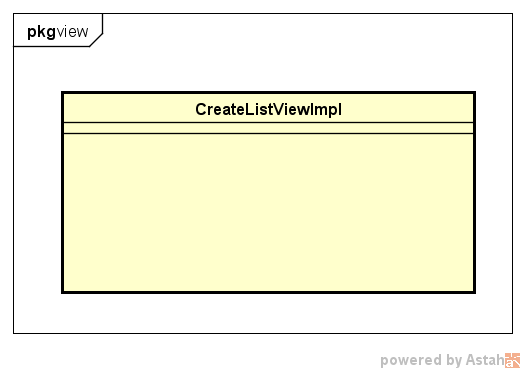
\includegraphics[scale=0.5]{Sezioni/Packages/App/create_list_view.png}
	\caption{Package application::feature::create\_list::view}
\end{figure}
\begin{itemize}
	\item \textbf{Descrizione}: package contenente la vista per la funzionalità di creazione di una lista
	\item \textbf{Classi e packages contenuti}:
	\begin{itemize}
	\item application::feature::create\_list::view::CreateListViewImpl: implementazione dell'interfaccia che rappresenta la vista per la funzionalità di creazione di una lista
	\end{itemize}
\end{itemize}

\subsubsection{Package application::feature::create\_list::presenter}
\label{Package application::feature::create_list::presenter}
\begin{figure}[H]
	\centering
	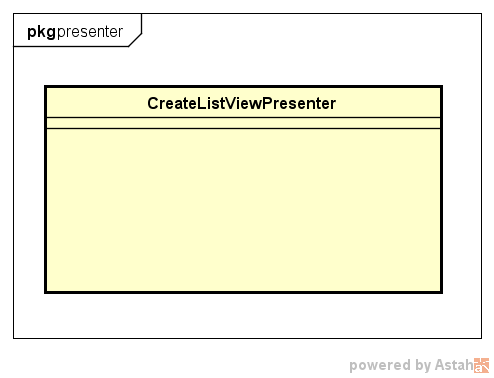
\includegraphics[scale=0.5]{Sezioni/Packages/App/create_list_presenter.png}
	\caption{Package application::feature::create\_list::presenter}
\end{figure}
\begin{itemize}
	\item \textbf{Descrizione}: package contenente il presenter per la vista di creazione di una lista
	\item \textbf{Classi e packages contenuti}:
	\begin{itemize}
	\item application::feature::create\_list::presenter::CreateListViewPresenter: classe che rappresenta il presenter per la vista di creazione di una lista
	\end{itemize}
\end{itemize}

\subsubsection{Package application::feature::forward}
\label{Package application::feature::forward}
\begin{figure}[H]
	\centering
	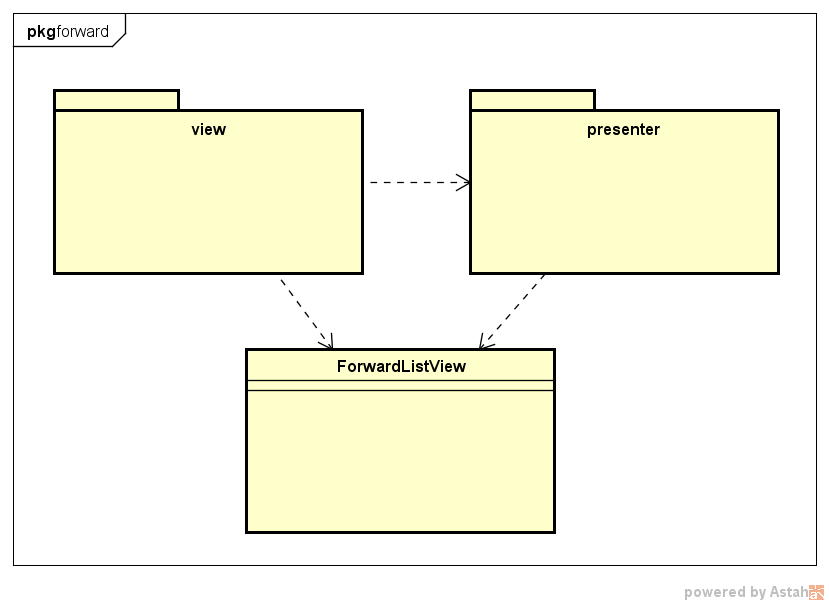
\includegraphics[scale=0.5]{Sezioni/Packages/App/forward.png}
	\caption{Package application::feature::forward}
\end{figure}
\begin{itemize}
	\item \textbf{Descrizione}: package contenente i componenti per la funzionalità di inoltro di una lista
	\item \textbf{Classi e packages contenuti}:
	\begin{itemize}
	\item application::feature::forward::view: package contenente la vista per la inoltro di una lista
	\item application::feature::forward::presenter: package contenente il presenter per la vista di inoltro di una lista
	\item application::feature::forward::ForwardListView: interfaccia rappresentante la vista per la funzionalità inoltro di una lista
	\end{itemize}
\end{itemize}

\subsubsection{Package application::feature::forward::view}
\label{Package application::feature::forward::view}
\begin{figure}[H]
	\centering
	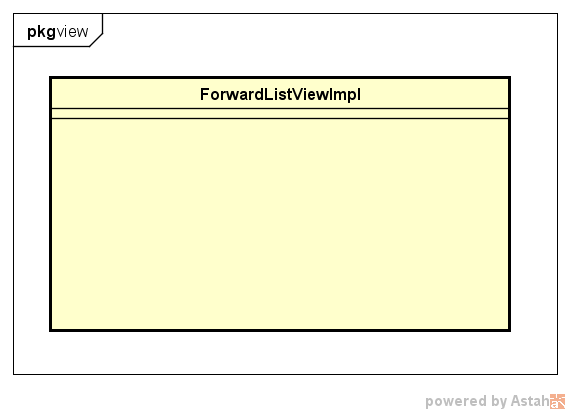
\includegraphics[scale=0.5]{Sezioni/Packages/App/forward_view.png}
	\caption{Package application::feature::forward::view}
\end{figure}
\begin{itemize}
	\item \textbf{Descrizione}: package contenente la vista per la funzionalità di inoltro di una lista
	\item \textbf{Classi e packages contenuti}:
	\begin{itemize}
	\item application::feature::forward::view::ForwardListViewImpl: implementazione dell'interfaccia che rappresenta la vista per la funzionalità di inoltro di una lista
	\end{itemize}
\end{itemize}

\subsubsection{Package application::feature::forward::presenter}
\label{Package application::feature::forward::presenter}
\begin{figure}[H]
	\centering
	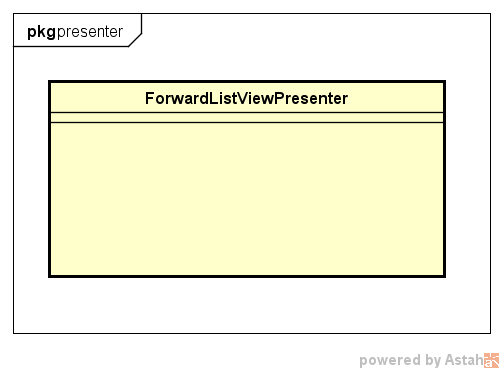
\includegraphics[scale=0.5]{Sezioni/Packages/App/forward_presenter.png}
	\caption{Package application::feature::forward::presenter}
\end{figure}
\begin{itemize}
	\item \textbf{Descrizione}: package contenente il presenter per la vista di inoltro di una lista
	\item \textbf{Classi e packages contenuti}:
	\begin{itemize}
	\item application::feature::forward::presenter::ForwardListViewPresenter: classe che rappresenta il presenter per la vista di inoltro di una lista
	\end{itemize}
\end{itemize}

\subsubsection{Package application::feature::input\_item\_info}
\label{Package application::feature::input_item_info}
\begin{figure}[H]
	\centering
	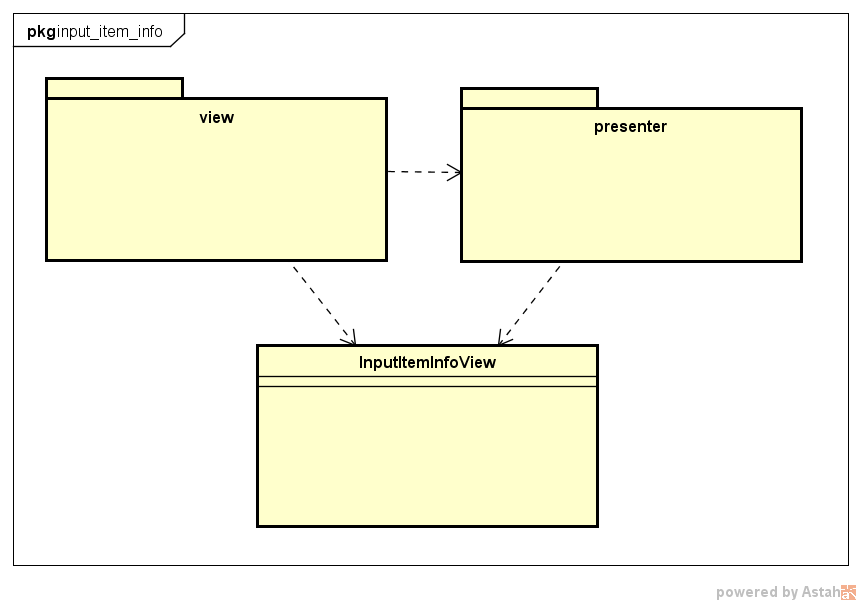
\includegraphics[scale=0.5]{Sezioni/Packages/App/input_item_info.png}
	\caption{Package application::feature::input\_item\_info}
\end{figure}
\begin{itemize}
	\item \textbf{Descrizione}: package contenente i componenti per la funzionalità di inserimento dati di un oggetto della lista
	\item \textbf{Classi e packages contenuti}:
	\begin{itemize}
	\item application::feature::input\_item\_info::view: package contenente la vista per la inserimento dati di un oggetto della lista
	\item application::feature::input\_item\_info::presenter: package contenente il presenter per la vista di inserimento dati di un oggetto della lista
	\item application::feature::input\_item\_info::InputItemInfoView: interfaccia rappresentante la vista per la funzionalità inserimento dati di un oggetto della lista
	\end{itemize}
\end{itemize}

\subsubsection{Package application::feature::input\_item\_info::view}
\label{Package application::feature::input_item_info::view}
\begin{figure}[H]
	\centering
	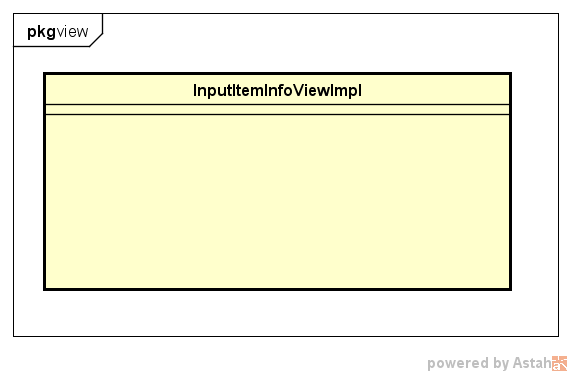
\includegraphics[scale=0.5]{Sezioni/Packages/App/input_item_info_view.png}
	\caption{Package application::feature::input\_item\_info::view}
\end{figure}
\begin{itemize}
	\item \textbf{Descrizione}: package contenente la vista per la funzionalità di inserimento dati di un oggetto della lista
	\item \textbf{Classi e packages contenuti}:
	\begin{itemize}
	\item application::feature::input\_item\_info::view::InputItemInfoViewImpl: implementazione dell'interfaccia che rappresenta la vista per la funzionalità di inserimento dati di un oggetto della lista
	\end{itemize}
\end{itemize}

\subsubsection{Package application::feature::input\_item\_info::presenter}
\label{Package application::feature::input_item_info::presenter}
\begin{figure}[H]
	\centering
	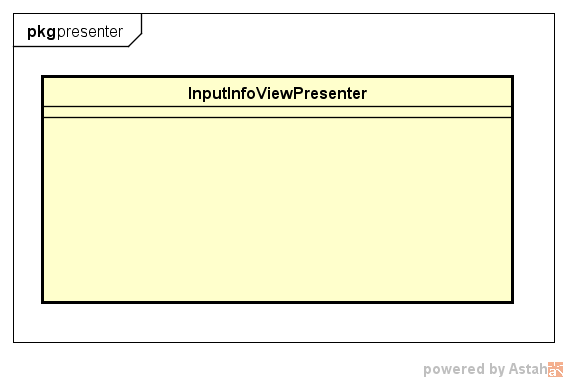
\includegraphics[scale=0.5]{Sezioni/Packages/App/input_item_info_presenter.png}
	\caption{Package application::feature::input\_item\_info::presenter}
\end{figure}
\begin{itemize}
	\item \textbf{Descrizione}: package contenente il presenter per la vista di inserimento dati di un oggetto della lista
	\item \textbf{Classi e packages contenuti}:
	\begin{itemize}
	\item application::feature::input\_item\_info::presenter::InputItemInfoViewPresenter: classe che rappresenta il presenter per la vista di inserimento dati di un oggetto della lista
	\end{itemize}
\end{itemize}


\subsubsection{Package application::feature::input\_list\_info}
\label{Package application::feature::input_list_info}
\begin{figure}[H]
	\centering
	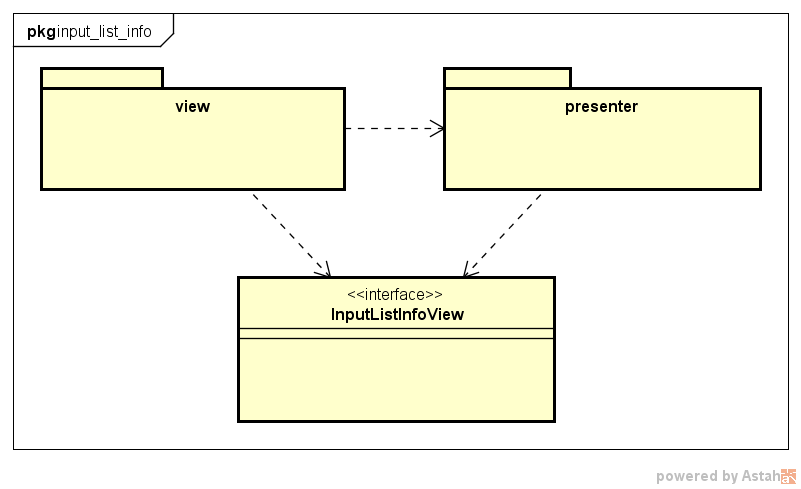
\includegraphics[scale=0.5]{Sezioni/Packages/App/input_list_info.png}
	\caption{Package application::feature::input\_list\_info}
\end{figure}
\begin{itemize}
	\item \textbf{Descrizione}: package contenente i componenti per la funzionalità di inserimento dati di una lista
	\item \textbf{Classi e packages contenuti}:
	\begin{itemize}
	\item application::feature::input\_list\_info::view: package contenente la vista per la inserimento dati di una lista
	\item application::feature::input\_list\_info::presenter: package contenente il presenter per la vista di inserimento dati di una lista
	\item application::feature::input\_list\_info::InputListInfoView: interfaccia rappresentante la vista per la funzionalità inserimento dati di una lista
	\end{itemize}
\end{itemize}

\subsubsection{Package application::feature::input\_list\_info::view}
\label{Package application::feature::input_list_info::view}
\begin{figure}[H]
	\centering
	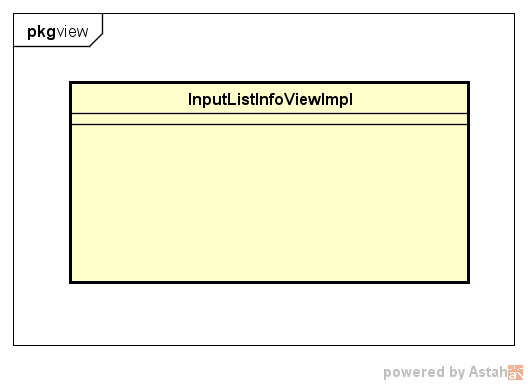
\includegraphics[scale=0.5]{Sezioni/Packages/App/input_list_info_view.png}
	\caption{Package application::feature::input\_list\_info::view}
\end{figure}
\begin{itemize}
	\item \textbf{Descrizione}: package contenente la vista per la funzionalità di inserimento dati di una lista
	\item \textbf{Classi e packages contenuti}:
	\begin{itemize}
	\item application::feature::input\_list\_info::view::InputListInfoViewImpl: implementazione dell'interfaccia che rappresenta la vista per la funzionalità di inserimento dati di una lista
	\end{itemize}
\end{itemize}

\subsubsection{Package application::feature::input\_list\_info::presenter}
\label{Package application::feature::input_list_info::presenter}
\begin{figure}[H]
	\centering
	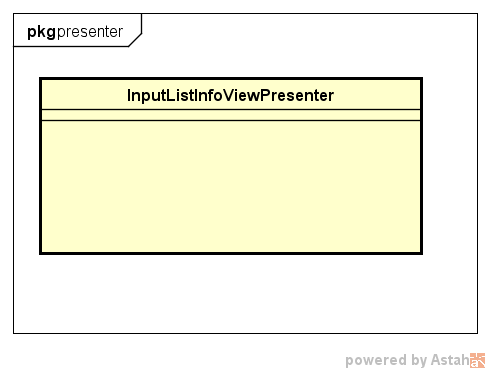
\includegraphics[scale=0.5]{Sezioni/Packages/App/input_list_info_presenter.png}
	\caption{Package application::feature::input\_list\_info::presenter}
\end{figure}
\begin{itemize}
	\item \textbf{Descrizione}: package contenente il presenter per la vista di inserimento dati di una lista
	\item \textbf{Classi e packages contenuti}:
	\begin{itemize}
	\item application::feature::input\_list\_info::presenter::InputListInfoViewPresenter: classe che rappresenta il presenter per la vista di inserimento dati di una lista
	\end{itemize}
\end{itemize}


\subsubsection{Package application::feature::modify\_item}
\label{Package application::feature::modify_item}
\begin{figure}[H]
	\centering
	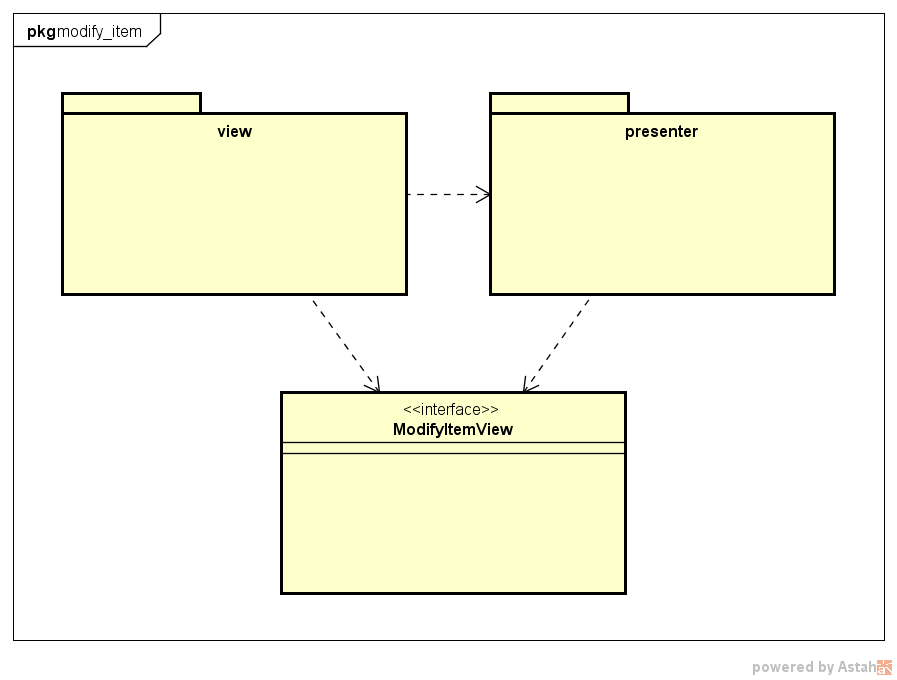
\includegraphics[scale=0.5]{Sezioni/Packages/App/modify_item.png}
	\caption{Package application::feature::modify\_item}
\end{figure}
\begin{itemize}
	\item \textbf{Descrizione}: package contenente i componenti per la funzionalità di modifica di un oggetto all'interno di una lista
	\item \textbf{Classi e packages contenuti}:
	\begin{itemize}
	\item application::feature::modify\_item::view: package contenente la vista per la modifica di un oggetto all'interno di una lista
	\item application::feature::modify\_item::presenter: package contenente il presenter per la vista di modifica di un oggetto all'interno di una lista
	\item application::feature::modify\_item::ModifyItemView: interfaccia rappresentante la vista per la funzionalità modifica di un oggetto all'interno di una lista
	\end{itemize}
\end{itemize}

\subsubsection{Package application::feature::modify\_item::view}
\label{Package application::feature::modify_item::view}
\begin{figure}[H]
	\centering
	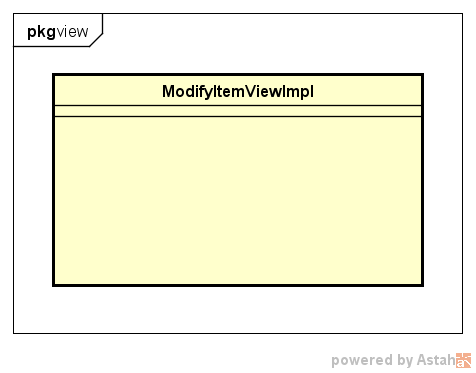
\includegraphics[scale=0.5]{Sezioni/Packages/App/modify_item_view.png}
	\caption{Package application::feature::modify\_item::view}
\end{figure}
\begin{itemize}
	\item \textbf{Descrizione}: package contenente la vista per la funzionalità di modifica di un oggetto all'interno di una lista
	\item \textbf{Classi e packages contenuti}:
	\begin{itemize}
	\item application::feature::modify\_item::view::ModifyItemViewImpl: implementazione dell'interfaccia che rappresenta la vista per la funzionalità di modifica di un oggetto all'interno di una lista
	\end{itemize}
\end{itemize}

\subsubsection{Package application::feature::modify\_item::presenter}
\label{Package application::feature::modify_item::presenter}
\begin{figure}[H]
	\centering
	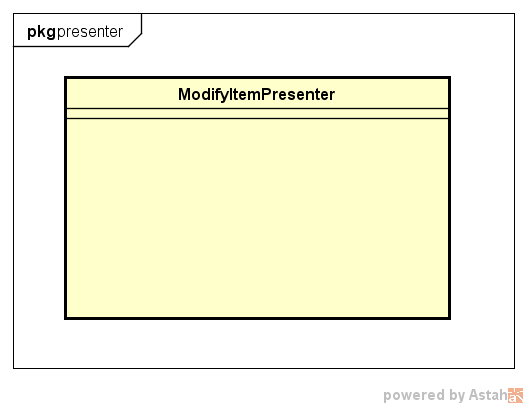
\includegraphics[scale=0.5]{Sezioni/Packages/App/modify_item_presenter.png}
	\caption{Package application::feature::modify\_item::presenter}
\end{figure}
\begin{itemize}
	\item \textbf{Descrizione}: package contenente il presenter per la vista di modifica di un oggetto all'interno di una lista
	\item \textbf{Classi e packages contenuti}:
	\begin{itemize}
	\item application::feature::modify\_item::presenter::ModifyItemViewPresenter: classe che rappresenta il presenter per la vista di modifica di un oggetto all'interno di una lista
	\end{itemize}
\end{itemize}


\subsubsection{Package application::feature::remove\_item}
\label{Package application::feature::remove_item}
\begin{figure}[H]
	\centering
	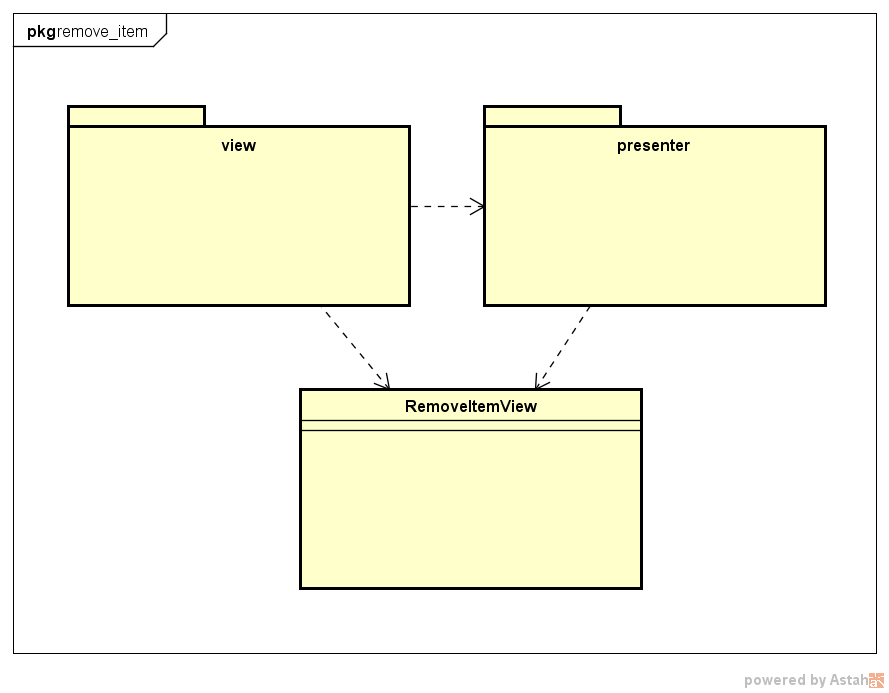
\includegraphics[scale=0.5]{Sezioni/Packages/App/remove_item.png}
	\caption{Package application::feature::remove\_item}
\end{figure}
\begin{itemize}
	\item \textbf{Descrizione}: package contenente i componenti per la funzionalità di rimozione di un oggetto da una lista
	\item \textbf{Classi e packages contenuti}:
	\begin{itemize}
	\item application::feature::remove\_item::view: package contenente la vista per la modifica di un oggetto all'interno di una lista
	\item application::feature::remove\_item::presenter: package contenente il presenter per la vista di modifica di un oggetto all'interno di una lista
	\item application::feature::remove\_item::RemoveItemView: interfaccia rappresentante la vista per la funzionalità modifica di un oggetto all'interno di una lista
	\end{itemize}
\end{itemize}

\subsubsection{Package application::feature::remove\_item::view}
\label{Package application::feature::remove_item::view}
\begin{figure}[H]
	\centering
	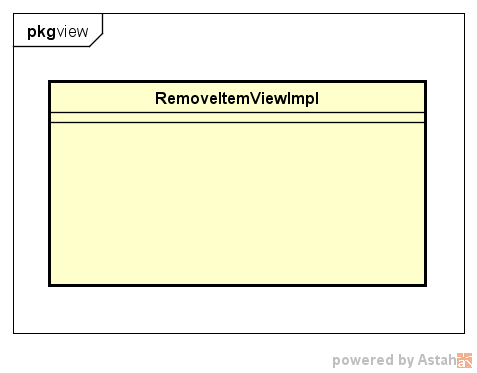
\includegraphics[scale=0.5]{Sezioni/Packages/App/remove_item_view.png}
	\caption{Package application::feature::remove\_item::view}
\end{figure}
\begin{itemize}
	\item \textbf{Descrizione}: package contenente la vista per la funzionalità di rimozione di un oggetto da una lista
	\item \textbf{Classi e packages contenuti}:
	\begin{itemize}
	\item application::feature::remove\_item::view::RemoveItemViewImpl: implementazione dell'interfaccia che rappresenta la vista per la funzionalità di rimozione di un oggetto da una lista
	\end{itemize}
\end{itemize}

\subsubsection{Package application::feature::remove\_item::presenter}
\label{Package application::feature::remove_item::presenter}
\begin{figure}[H]
	\centering
	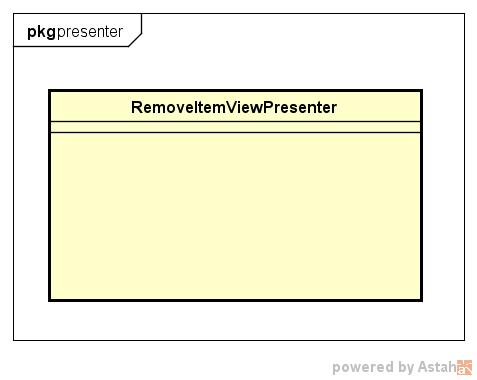
\includegraphics[scale=0.5]{Sezioni/Packages/App/remove_item_presenter.png}
	\caption{Package application::feature::forward::remove\_item::presenter}
\end{figure}
\begin{itemize}
	\item \textbf{Descrizione}: package contenente il presenter per la vista di rimozione di un oggetto da una lista
	\item \textbf{Classi e packages contenuti}:
	\begin{itemize}
	\item application::feature::remove\_item::presenter::RemoveItemViewPresenter: classe che rappresenta il presenter per la vista di rimozione di un oggetto da una lista
	\end{itemize}
\end{itemize}


\subsubsection{Package application::feature::sharewithcontact}
\label{Package application::feature::sharewithcontact}
\begin{figure}[H]
	\centering
	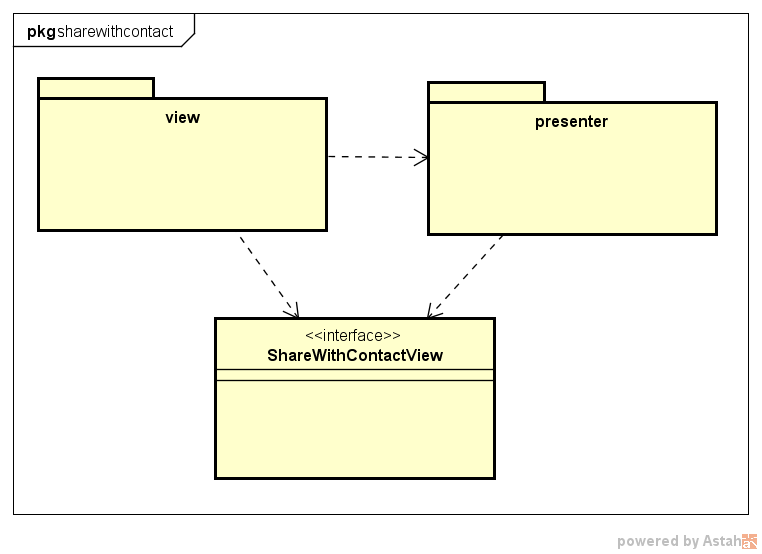
\includegraphics[scale=0.5]{Sezioni/Packages/App/share_with_contact.png}
	\caption{Package application::feature::sharewithcontact}
\end{figure}
\begin{itemize}
	\item \textbf{Descrizione}: package contenente i componenti per la funzionalità di condivisione della lista con un contatto
	\item \textbf{Classi e packages contenuti}:
	\begin{itemize}
	\item application::feature::sharewithcontact::view: package contenente la vista per la modifica di un oggetto all'interno di una lista
	\item application::feature::sharewithcontact::presenter: package contenente il presenter per la vista di modifica di un oggetto all'interno di una lista
	\item application::feature::sharewithcontact::ShareWithContactView: interfaccia rappresentante la vista per la funzionalità modifica di un oggetto all'interno di una lista
	\end{itemize}
\end{itemize}

\subsubsection{Package application::feature::sharewithcontact::view}\label{Package application::feature::sharewithcontact::view}
\begin{figure}[H]
	\centering
	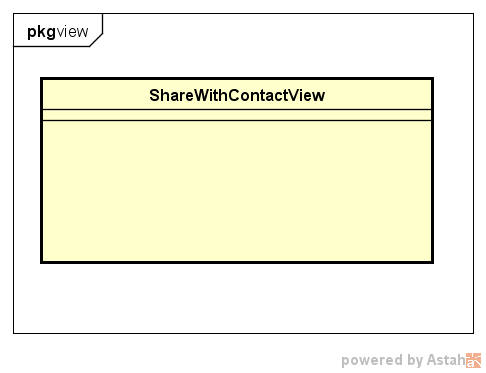
\includegraphics[scale=0.5]{Sezioni/Packages/App/share_with_contact_view.png}
	\caption{Package application::feature::sharewithcontact::view}
\end{figure}
\begin{itemize}
	\item \textbf{Descrizione}: package contenente la vista per la funzionalità di condivisione della lista con un contatto
	\item \textbf{Classi e packages contenuti}:
	\begin{itemize}
	\item application::feature::sharewithcontact::view::ShareWithContactViewImpl: implementazione dell'interfaccia che rappresenta la vista per la funzionalità di condivisione della lista con un contatto
	\end{itemize}
\end{itemize}

\subsubsection{Package application::feature::sharewithcontact::presenter}
\label{Package application::feature::sharewithcontact::presenter}
\begin{figure}[H]
	\centering
	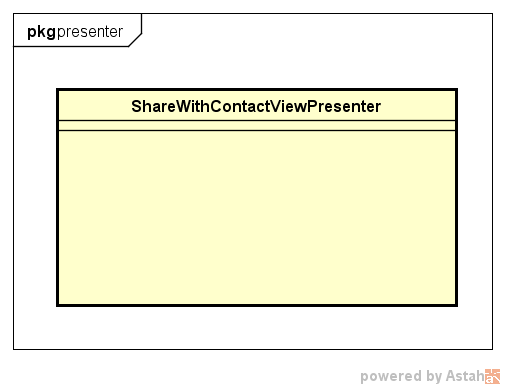
\includegraphics[scale=0.5]{Sezioni/Packages/App/share_with_contact_presenter.png}
	\caption{Package application::feature::sharewithcontact::presenter}
\end{figure}
\begin{itemize}
	\item \textbf{Descrizione}: package contenente il presenter per la vista di condivisione della lista con un contatto
	\item \textbf{Classi e packages contenuti}:
	\begin{itemize}
	\item application::feature::sharewithcontact::presenter::ShareWithContactViewPresenter: classe che rappresenta il presenter per la vista di condivisione della lista con un contatto
	\end{itemize}
\end{itemize}


\subsubsection{Package application::feature::sharewithgroup}
\label{Package application::feature::sharewithgroup}
\begin{figure}[H]
	\centering
	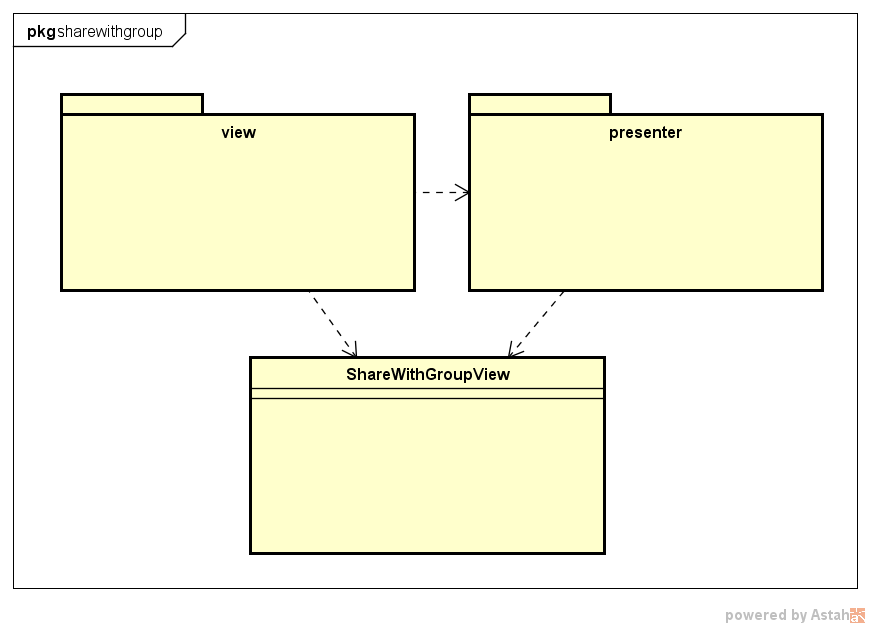
\includegraphics[scale=0.5]{Sezioni/Packages/App/share_with_group.png}
	\caption{Package application::feature::sharewithgroup}
\end{figure}
\begin{itemize}
	\item \textbf{Descrizione}: package contenente i componenti per la funzionalità di condivisione della lista con un gruppo
	\item \textbf{Classi e packages contenuti}:
	\begin{itemize}
	\item application::feature::sharewithgroup::view: package contenente la vista per la modifica di un oggetto all'interno di una lista
	\item application::feature::sharewithgroup::presenter: package contenente il presenter per la vista di modifica di un oggetto all'interno di una lista
	\item application::feature::sharewithgroup::ShareWithGroupView: interfaccia rappresentante la vista per la funzionalità modifica di un oggetto all'interno di una lista
	\end{itemize}
\end{itemize}

\subsubsection{Package application::feature::sharewithgroup::view}
\label{Package application::feature::sharewithgroup::view}
\begin{figure}[H]
	\centering
	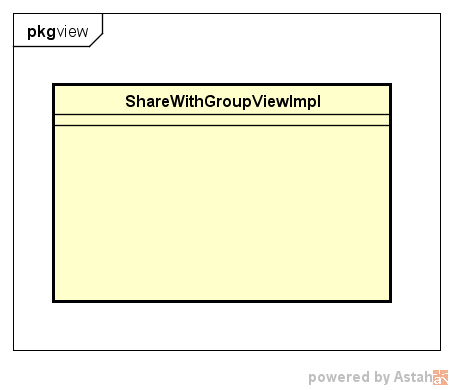
\includegraphics[scale=0.5]{Sezioni/Packages/App/share_with_group_view.png}
	\caption{Package application::feature::sharewithgroup::view}
\end{figure}
\begin{itemize}
	\item \textbf{Descrizione}: package contenente la vista per la funzionalità di condivisione della lista con un gruppo
	\item \textbf{Classi e packages contenuti}:
	\begin{itemize}
	\item application::feature::sharewithgroup::view::ShareWithGroupViewImpl: implementazione dell'interfaccia che rappresenta la vista per la funzionalità di condivisione della lista con un gruppo
	\end{itemize}
\end{itemize}

\subsubsection{Package application::feature::sharewithgroup::presenter}
\label{Package application::feature::sharewithgroup::presenter}
\begin{figure}[H]
	\centering
	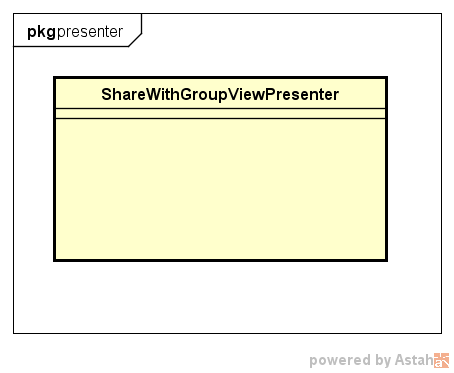
\includegraphics[scale=0.5]{Sezioni/Packages/App/share_with_group_presenter.png}
	\caption{Package application::feature::sharewithgroup::presenter}
\end{figure}
\begin{itemize}
	\item \textbf{Descrizione}: package contenente il presenter per la vista di condivisione della lista con un gruppo
	\item \textbf{Classi e packages contenuti}:
	\begin{itemize}
	\item application::feature::sharewithgroup::presenter::ShareWithGroupViewPresenter: classe che rappresenta il presenter per la vista di condivisione della lista con un gruppo
	\end{itemize}
\end{itemize}


\subsubsection{Package application::feature::help}
\label{Package application::feature::help}
\begin{figure}[H]
	\centering
	\includegraphics[scale=0.5]{Sezioni/Packages/App/help.png}
	\caption{Package application::feature::help}
\end{figure}
\begin{itemize}
	\item \textbf{Descrizione}: package contenente i componenti per la funzionalità di visualizzazione aiuto per l'utilizzo dell'applicazione
	\item \textbf{Classi e packages contenuti}:
	\begin{itemize}
	\item application::feature::help::view: package contenente la vista per la modifica di un oggetto all'interno di una lista
	\item application::feature::help::presenter: package contenente il presenter per la vista di modifica di un oggetto all'interno di una lista
	\item application::feature::help::helpView: interfaccia rappresentante la vista per la funzionalità modifica di un oggetto all'interno di una lista
	\end{itemize}
\end{itemize}

\subsubsection{Package application::feature::help::view}
\label{Package application::feature::help::view}
\begin{figure}[H]
	\centering
	\includegraphics[scale=0.5]{Sezioni/Packages/App/help_view.png}
	\caption{Package application::feature::help::view}
\end{figure}
\begin{itemize}
	\item \textbf{Descrizione}: package contenente la vista per la funzionalità di visualizzazione aiuto per l'utilizzo dell'applicazione
	\item \textbf{Classi e packages contenuti}:
	\begin{itemize}
	\item application::feature::help::view::helpViewImpl: implementazione dell'interfaccia che rappresenta la vista per la funzionalità di visualizzazione aiuto per l'utilizzo dell'applicazione
	\end{itemize}
\end{itemize}

\subsubsection{Package application::feature::help::presenter}
\label{Package application::feature::help::presenter}
\begin{figure}[H]
	\centering
	\includegraphics[scale=0.5]{Sezioni/Packages/App/help_presenter.png}
	\caption{Package application::feature::help::presenter}
\end{figure}
\begin{itemize}
	\item \textbf{Descrizione}: package contenente il presenter per la vista di visualizzazione aiuto per l'utilizzo dell'applicazione
	\item \textbf{Classi e packages contenuti}:
	\begin{itemize}
	\item application::feature::help::presenter::helpViewPresenter: classe che rappresenta il presenter per la vista di visualizzazione aiuto per l'utilizzo dell'applicazione
	\end{itemize}
\end{itemize}

\subsubsection{Package application::feature::exception}
\label{Package application::feature::exception}
\begin{figure}[H]
	\centering
	\includegraphics[scale=0.5]{Sezioni/Packages/App/exception.png}
	\caption{Package application::feature::exception}
\end{figure}
\begin{itemize}
	\item \textbf{Descrizione}: package contenente tutte le eccezioni che l'applicazione può lanciare durante l'esecuzione
	\item \textbf{Classi e packages contenuti}:
	\begin{itemize}
	\item application::feature::exception::Exception: classe che rappresenta una eccezione generica
	\item application::feature::exception::BadParameterException: classe che rappresenta una eccezione lanciata nel qual caso un parametro di un metodo sia incorretto
	\end{itemize}
\end{itemize}


\newpage
\newpage
\section{Diagramma delle classi}

\subsection{SDK}

\subsubsection{BaseBubble}

\label{BaseBubble}
\begin{figure}[ht]
	\centering
	\includegraphics[scale=0.5]{Sezioni/SottosezioniST/img/BaseBubble.png}
	\caption{BaseBubble}
\end{figure}

\begin{itemize}
\item \textbf{Descrizione:} Classe base astratta che rappresenta le bolle di Monolith.
\item \textbf{Utilizzo:} Classe base astratta utilizzata ed estesa ogni qualvolta uno sviluppatore intende creare nuove bolle.
\item \textbf{Attributi:} 
\begin{itemize}
\item \textit{protected layout:VerticalLayoutView}\\
Oggetto che rappresenta il layout verticale della bolla.
\end{itemize}
\item \textbf{Metodi:}
\begin{itemize}
\item \textit{public addComponent(component:BaseComponent):void}\\
Aggiunge un widget alla bolla.
\item{\textbf{Parametri}: \begin{itemize}
\item \textit{component:BaseComponent}\\
Oggetto che rappresenta il componente che si desidera aggiungere alla bolla.
\end{itemize}}
\item \textit{public renderView():string}\\
Genera il codice HTML, CSS e JavaScript necessario per visualizzare bolle.
\end{itemize}
\end{itemize}

\subsubsection{ToDoListBubble}

\label{ToDoListBubble}
\begin{figure}[ht]
	\centering
	\includegraphics[scale=0.5]{Sezioni/SottosezioniST/img/ToDoListBubble.png}
	\caption{ToDoListBubble}
\end{figure}

\begin{itemize}
\item \textbf{Descrizione:} Classe concreta che estende BaseBubble, destinata alla creazione di bolle lista di Monolith.
\item \textbf{Utilizzo:} Classe utilizzata ogni qualvolta uno sviluppatore intende creare nuove bolle lista.
\item \textbf{Attributi:}
\begin{itemize}
\item \textit{private textView:TextWidgetView}\\
Oggetto che rappresenta il widget contenente il testo della bolla lista.
\item \textit{private checklist:CheckListView}\\
Oggetto che rappresenta il widget contenente la lista di oggetti che si possono spuntare.
\end{itemize}
\item \textbf{Metodi:}
\begin{itemize}
\item \textit{public ToDoListBubble():ToDoListBubble}\\
Il costruttore della classe ToDoListBubble.
\item \textit{public addItem(item:string):void}\\
Aggiunge un elemento con il nome definito alla bolla lista.
\item{\textbf{Parametri}: \begin{itemize}
\item \textit{item:string}\\
Valore che rappresenta il nome dell'elemento che si vuole aggiungere alla lista.
\end{itemize}}
\end{itemize}
\end{itemize}

\subsubsection{MarkdownBubble}

\label{MarkdownBubble}
\begin{figure}[ht]
	\centering
	\includegraphics[scale=0.5]{Sezioni/SottosezioniST/img/MarkdownBubble.png}
	\caption{MarkDownBubble}
\end{figure}

\begin{itemize}
\item \textbf{Descrizione:} Classe concreta che estende BaseBubble, destinata alla creazione di bolle testo markdown di Monolith.
\item \textbf{Utilizzo:} Classe utilizzata ogni qualvolta uno sviluppatore intende creare nuove bolle testo markdown.
\item \textbf{Attributi:}
\begin{itemize}
\item \textit{private textview:TextWidgetView}\\
Oggetto che rappresenta il widget contenente il testo della bolla testo markdown.
\end{itemize}
\item \textbf{Metodi:}
\begin{itemize}
\item \textit{public MarkdownBubble():MarkdownBubble}\\
Il costruttore della classe MarkdownBubble.
\item \textit{public setText(text:string):void}\\
Imposta il testo della bolla lista con il valore definito.
\item{\textbf{Parametri}: \begin{itemize}
\item \textit{text:string}\\
Valore che rappresenta il testo che si vuole inserire nella bolla testo markdown.
\end{itemize}}
\end{itemize}
\end{itemize}

\subsubsection{AlertBubble}

\label{AlertBubble}
\begin{figure}[ht]
	\centering
	\includegraphics[scale=0.5]{Sezioni/SottosezioniST/img/AlertBubble.png}
	\caption{AlertBubble}
\end{figure}

\begin{itemize}
\item \textbf{Descrizione:} Classe concreta che estende BaseBubble, destinata alla creazione di bolle avviso di Monolith.
\item \textbf{Utilizzo:} Classe utilizzata ogni qualvolta uno sviluppatore intende creare nuove bolle avviso.
\item \textbf{Attributi:} 
\begin{itemize}
\item \textit{private titleView:TextWidgetView}\\
Campo che rappresenta e contiene il titolo della bolla avviso.
\item \textit{private messageView:TextWidgetView}\\
Campo che rappresenta e contiene il messaggio della bolla avviso.
\end{itemize}
\item \textbf{Metodi:}
\begin{itemize}
\item \textit{public AlertBubble():AlertBubble}\\
Il costruttore della classe AlertBubble.
\item \textit{public setTitle(title:string):void}\\
Imposta il titolo della bolla avviso con il valore title.
\item{\textbf{Parametri}: \begin{itemize}
\item \textit{title:string}\\
Valore che rappresenta il titolo che si vuole impostare alla bolla avviso.
\end{itemize}}
\item \textit{public setMessage(message:string):void}\\
Imposta il messaggio della bolla avviso con il valore message.
\item{\textbf{Parametri}: \begin{itemize}
\item \textit{message:string}\\
Valore che rappresenta il messaggio testuale che si vuole impostare alla bolla avviso.
\end{itemize}}
\end{itemize}
\end{itemize}
\subsubsection{BaseComponent}

\label{BaseComponent}
\begin{figure}[ht]
	\centering
	\includegraphics[scale=0.5]{Sezioni/SottosezioniST/img/BaseComponent.png}
	\caption{BaseComponent}
\end{figure}

\begin{itemize}
\item \textbf{Descrizione:} Interfaccia base che rappresenta un qualsiasi oggetto che può essere inserito all'interno di un bolla.
\item \textbf{Utilizzo:} Interfaccia che viene implementata ogni qualvolta uno sviluppatore intende inserire all'interno di un bolla un widget o un layout.
\item \textbf{Attributi:}
\item \textbf{Metodi:}
\begin{itemize}
\item \textit{public renderView():string}\\
Genera il codice HTML, CSS e JavaScript necessario per visualizzare BaseComponent.
\end{itemize}
\end{itemize}
\subsubsection{monolith::client::events::ChecklistCompleteEmitter}

\label{monolith::client::events::ChecklistCompleteEmitter}
\begin{figure}[H]
	\centering
	\includegraphics[scale=0.5]{Sezioni/SottosezioniST/img/ChecklistCompleteEmitter.png}
	\caption{monolith::client::events::ChecklistCompleteEmitter}
\end{figure}

\begin{itemize}
\item \textbf{Descrizione:} Classe che contiene l'emettitore di eventi da lanciare quando una checklist viene completata. Estende Event-Emitter (es6-event-emitter).
\item \textbf{Utilizzo:} La classe viene utilizzata ogniqualvolta una checklist viene completata, lanciando l'evento corrispondente.
\item \textbf{Attributi:}
\item \textbf{Metodi:}
\begin{itemize}
\item \textit{public emitChecklistComplete(id:string):void}\\
Questo metodo emette l'evento relativo al completamento di una lista.
			\\ \textbf{Parametri}: \begin{itemize}
			\item \textit{id:string}\\
			L'identificativo della lista che è stata completata
			\end{itemize} 
\end{itemize}
\end{itemize}

\subsubsection{monolith::client::events::ChecklistUpdateEmitter}

\label{monolith::client::events::ChecklistUpdateEmitter}
\begin{figure}[H]
	\centering
	\includegraphics[scale=0.5]{Sezioni/SottosezioniST/img/ChecklistUpdateEmitter.png}
	\caption{monolith::client::events::ChecklistUpdateEmitter}
\end{figure}

\begin{itemize}
\item \textbf{Descrizione:} Classe che contiene l'emettitore di eventi da lanciare quando gli elementi di una checklist vengono cliccati. Estende Event-Emitter (es6-event-emitter).
\item \textbf{Utilizzo:} La classe viene utilizzata ogniqualvolta un elemento di una checklist viene cliccato, lanciando l'evento corrispondente.
\item \textbf{Attributi:}
\item \textbf{Metodi:}
\begin{itemize}
\item \textit{public emitOnUpdate(id:string,string:string):void}\\
Questo metodo emette l'evento relativo al click di un elemento di una lista.
			\\ \textbf{Parametri}: \begin{itemize}
			\item \textit{id:string}\\
			L'identificativo della lista della quale è stato cliccato un elemento.
			\item \textit{string:string}\\
			Stringa che contiene l'informazione relativa al tipo di click effettuato, se normale o prolungato.
			\end{itemize} 
\end{itemize}
\end{itemize}

\subsubsection{monolith::client::events::ClickButtonEventEmitter}

\label{monolith::client::events::ClickButtonEventEmitter}
\begin{figure}[H]
	\centering
	\includegraphics[scale=0.5]{Sezioni/SottosezioniST/img/ClickButtonEventEmitter.png}
	\caption{monolith::client::events::ClickButtonEventEmitter}
\end{figure}

\begin{itemize}
\item \textbf{Descrizione:} Classe che contiene l'emettitore di eventi da lanciare quando un bottone viene cliccato. Estende Event-Emitter (es6-event-emitter).
\item \textbf{Utilizzo:} La classe viene utilizzata ogniqualvolta un bottone viene cliccato.
\item \textbf{Attributi:}
\item \textbf{Metodi:}
\begin{itemize}
\item \textit{public emitClickButtonEvent():void}\\
Questo metodo emette l'evento relativo al click di un bottone.
\item \textit{public emitLongClickButtonEvent():void}\\
Questo metodo emette l'evento relativo al click prolungato di un bottone.
\end{itemize}
\end{itemize}
\subsubsection{monolith::client::component::layout::BaseLayout}

\label{monolith::client::component::layout::BaseLayout}
\begin{figure}[ht]
	\centering
	\includegraphics[scale=0.5]{Sezioni/SottosezioniST/img/BaseLayout.png}
	\caption{monolith::client::component::layout::BaseLayout}
\end{figure}

\begin{itemize}
\item \textbf{Descrizione:} Classe astratta che implementa l'interfaccia BaseComponent e che rappresenta un oggetto layout per la disposizione di componenti nelle bolle di Monolith.
\item \textbf{Utilizzo:} Classe utilizzata ed estesa ogni qualvolta uno sviluppatore intende creare un nuovo layout da inserire in una bolla.
\item \textbf{Attributi:}
\begin{itemize}
\item \textit{private items:List<BaseComponent>}\\
Rappresenta la lista di oggetti BaseComponent contenuti nel layout.
\end{itemize}
\item \textbf{Metodi:}
\begin{itemize}
\item \textit{public addItem(component:BaseComponent):void}\\
Aggiunge un oggetto BaseComponent al layout.
\\ \textbf{Parametri}: \begin{itemize}
\item \textit{component:BaseComponent}\\
Oggetto che rappresenta il BaseComponent da aggiungere al layout.
\end{itemize}
\end{itemize}
\end{itemize}

\subsubsection{monolith::client::component::layout::vertical::VerticalLayoutView}

\label{monolith::client::component::layout::vertical::VerticalLayoutView}
\begin{figure}[H]
	\centering
	\includegraphics[scale=0.5]{Sezioni/SottosezioniST/img/VerticalLayoutView.png}
	\caption{monolith::client::component::layout::vertical::VerticalLayoutView}
\end{figure}

\begin{itemize}
\item \textbf{Descrizione:} Classe concreta che estende BaseLayout, destinata alla creazione di layout per la disposizione verticale di BaseComponent.
\item \textbf{Utilizzo:} Classe utilizzata ogni qualvolta uno sviluppatore intende creare un nuovo layout orizzontale da inserire in una bolla.
\item \textbf{Attributi:}
\item \textbf{Metodi:}
\begin{itemize}
\item\textit{public VerticalLayoutView():VerticalLayoutView}\\
Il costruttore per la classe VerticalLayoutView.
\item \textit{public addItem(component:BaseComponent):void}\\
Aggiunge un oggetto BaseComponent al layout verticale.
\\ \textbf{Parametri}: \begin{itemize}
\item \textit{component:BaseComponent}\\
Oggetto che rappresenta il BaseComponent da aggiungere al layout verticale.
\end{itemize}
\item \textit{public renderView():HtmlDOMElement}\\
Restituisce l'elemento DOM rappresentante i BaseComponent disposti nel layout verticale.
\end{itemize}
\end{itemize}

\subsubsection{monolith::client::component::layout::horizontal::HorizontalLayoutView}

\label{monolith::client::component::layout::horizontal::HorizontalLayoutView}
\begin{figure}[H]
	\centering
	\includegraphics[scale=0.5]{Sezioni/SottosezioniST/img/HorizontalLayoutView.png}
	\caption{monolith::client::component::layout::horizontal::HorizontalLayoutView}
\end{figure}

\begin{itemize}
\item \textbf{Descrizione:} Classe concreta che estende BaseLayout, destinata alla creazione di layout  per la disposizione orizzontale di BaseComponent.
\item \textbf{Utilizzo:} Classe utilizzata ogni qualvolta uno sviluppatore intende creare un nuovo layout verticale da inserire in una bolla.
\item \textbf{Attributi:}
\item \textbf{Metodi:}
\begin{itemize}
\item\textit{public HorizontalLayoutView():HorizontalLayoutView}\\
Il costruttore per la classe HorizontalLayoutView.
\item \textit{private createColumn():Object}\\
Crea una colonna per la disposizione degli oggetti in senso orizzontale del layout
\item \textit{public addItem(component:BaseComponent):void}\\
Aggiunge un oggetto BaseComponent al layout orizzontale.
\\ \textbf{Parametri}: \begin{itemize}
\item \textit{component:BaseComponent}\\
Oggetto che rappresenta il BaseComponent da aggiungere al layout orizzontale.
\end{itemize}
\item \textit{public renderView():HtmlDOMElement}\\
Restituisce l'elemento DOM rappresentante i BaseComponent disposti nel layout orizzontale.
\end{itemize}
\end{itemize}
\subsection{Widgets}
\subsubsection{TextWidget}
\begin{lstlisting}[language=JavaScript]
// Create a TextWidget
let textWidget = new Monolith.Widget.TextWidget;

// Hide the widget
textWidget.setVisibility(false); // Default is true, which will show is

// Set the text. Markdown notation is also supported
textWidget.setText("Foo");
textWidget.setText("Markdown __is supported__ **too**");

// Set the text color using HEX notation (http://www.color-hex.com/)
textWidget.setTextColor("#C61A10");

// Set the text size in pixel
textWidget.setTextSize(15);

// Set the URL highlighting color
textWidget.setUrlHighligthColor("#EE42F4");

// Enable or disable the text formatting, this includes also URL highlighting
textWidget.setFormatText(true);
textWidget.setFormatText(false);
\end{lstlisting}
~\\~\\

\subsubsection{ImageWidget}
\begin{lstlisting}[language=JavaScript]
// Create the ImageWidget
let imageWidget = new Monolith.Widget.ImageWidget;

// Hide the widget
imageWidget.setVisibility(false); // Default is true, which will show is

// Set the image associated with the widget
imageWidget.setImage("path/to/image.png");

// Set the image dimensions
imageWidget.setWidth(200);
imageWidget.setHeight(50);
\end{lstlisting}

\newpage
\subsubsection{ButtonWidget}
\begin{lstlisting}[language=JavaScript]
// Create a ButtonWidget
let buttonWidget = new Monolith.Widget.ButtonWidget;

// Set the dimensions of the button
buttonWidget.setWidth(100);
buttonWidget.setHeight(50);

// Set the color of the button
buttonWidget.setBackgroundColor("#41F492");

// Set the action associated with the button
buttonWidget.setOnClickAction(function(){
    alert("The button has been clicked");
});

// Set the action associated with the button when the user long-clicks it
buttonWidget.setOnLongClickAction(function(){
    alert("The button has been long clicked");
});

// Set the milliseconds that need to pass before a click is considered a long click
buttonWidget.setOnLongClickActionTimer(500);
\end{lstlisting}
~\\~\\

\subsubsection{ListWidget}
\begin{lstlisting}[language=JavaScript]
// Create the ListWidget
let listWidget = new Monolith.Widget.ListWidget;

// Add items to the list
listWidget.addItem("First");
listWidget.addItem("Second");
listWidget.addItem("Third");

// Set the indicator of the list
listWidget.setCharacterNumber(); // Numbered list
listWidget.setCharacterCircle(); // Unnumbered list

// Set the indicator color
listWidget. setColor("#292929");
\end{lstlisting}

\newpage
\subsubsection{CheckListItemWidget}
\begin{lstlisting}[language=JavaScript]
// Create a new CheckListItemWidget
let checkListItemWidget = new Monolith.Widget.CheckListItemWidget;

// Set the text associated with the item
checkListItemWidget.setText("Click me!");

// Customize the check appereance
// Color the check box instead of using a check tick
checkListItemWidget.setUseSelectionMark(true); 
// Set the color that will be used to color the check box
checkListItemWidget.setSelectionColor("#AAAAAA"); 
// Use a check tick
checkListItemWidget.setUseSelectionMark(false); 
// Set the character used as check tick
checkListItemWidget.setSelectionCharacter("X"); 

// Check or un-check the option
checkListItemWidget.setChecked(true); // Checked
checkListItemWidget.setChecked(false); // Un-checked

// Know it the option is checked or not
let isChecked = checkListItemWidget.isChecked();
if (isChecked){
    // The option is checked
} else {
    // The option is not checked
}


// Set the action to perform on click
checkListItemWidget.setOnClick(function(item){
    // The item parameter represents the view of the item that has been clicked
    item.setText("New text after click");
});

// Set the action to perform after a long click (1000 ms)
checkListItemWidget.setOnLongClick(function(){
    // The item parameter represents the view of the item that has been clicked
   item.setText("New text after long click");
});


// Delete the item
checkListItemWidget.removeOption();
\end{lstlisting}

\newpage
\subsubsection{Create a custom widget}
In order to create a new custom widget and add it to \termine{Monolith} so than you can use it like the default ones, you have to do as follows.
\begin{enumerate}

	\item Create a new class which extends from \texttt{BaseWidget}
\begin{lstlisting}[language=JavaScript]
export class MyWidget extends Monolith.Widget.BaseWidget {

    constructor(){
        super(); // You need to call this to create the above hierarchy
        
        // Initialize your widget here
    }
    
    renderView(){
        // Renders the view of the widget and returns a DOMElement object
    }

    performOperation(){
        // Perform some operation
    }

}
\end{lstlisting}

	\item Use your widget wherever you want
\begin{lstlisting}[language=JavaScript]
// Import the widget
import {MyWidget} from '/path/to/MyWidget.js';

// Istantiate the widget
let myWidget = new MyWidget();

// Perform operations with the widget
myWidget.performOperation();

// Render the widget's view
myWidget.renderView();
\end{lstlisting}
  
\end{enumerate}  
  
\textbf{Note} \\ 
The default widget's behaviour does \textbf{not} let the user use a single widget without a bubble container that holds it. \\
If you plan to render the widget's view inside a Rocket.chat room, please create a bubble and add your widget to the bubble, so that the bubble will render it and show it to the user.

\newpage



\subsection{Applicazione demo lista-spesa}

\subsubsection{feature::GeneralView}

\label{feature::GeneralView}
\begin{figure}[H]
	\centering
	\includegraphics[scale=0.5]{Sezioni/SottosezioniST/img/app/GeneralView.png}
	\caption{feature::GeneralView}
\end{figure}

\begin{itemize}
\item \textbf{Descrizione}: Interfaccia che sta alla base della gerarchia delle componenti della lista-spesa.
\item \textbf{Utilizzo}:
\item \textbf{Attributi}: 
\item \textbf{Metodi}:
	\begin{itemize}
	\item \textit{public renderView():string}\\
	Genera il codice HTML CSS JS necessario per visualizzare una componente grafica della lista-spesa.
	\end{itemize}
\item \textbf{Eventi}:
\end{itemize}

\subsubsection{feature::remove\_item::RemoveItemView}

\label{feature::remove_item::RemoveItemView}
\begin{figure}[H]
	\centering
	\includegraphics[scale=0.5]{Sezioni/SottosezioniST/img/app/RemoveItemView.png}
	\caption{feature::remove\_item::RemoveItemView}
\end{figure}

\begin{itemize}
\item \textbf{Descrizione}: Questa interfaccia rappresenta la view relativa alla rimozione di un oggetto dalla lista-spesa.
\item \textbf{Utilizzo}: L'interfaccia viene utilizzata per disaccoppiare presenter e implementazione della rimozione, visualizza i dati che gli vengono passati dal presenter.
\item \textbf{Attributi}: 
\item \textbf{Metodi}:
\item \textbf{Eventi}:
	\begin{itemize}	
	\item \textit{public onItemRemoveClicked(item:ListItem):void}\\
	Evento che rappresenta il click, da parte dell'utente, sull'oggetto visuale necessario alla rimozione di un oggetto dalla lista.
			\\ \textbf{Parametri}: \begin{itemize}
			\item \textit{item:ListItem}\\
			L'oggetto che è stato cliccato e che l'utente desidera rimuoverlo dalla lista.
			\end{itemize} 
	\end{itemize}
\end{itemize}

\subsubsection{feature::remove\_item::view::RemoveItemViewImpl}

\label{feature::remove_item::view::RemoveItemViewImpl}
\begin{figure}[H]
	\centering
	\includegraphics[scale=0.5]{Sezioni/SottosezioniST/img/app/RemoveItemViewImpl.png}
	\caption{feature::remove\_item::view::RemoveItemViewImpl}
\end{figure}

\begin{itemize}
\item \textbf{Descrizione}: Questa classe rappresenta la vista per la rimozione di un oggetto dalla lista-spesa, implementando l'interfaccia RemoveItemView.
\item \textbf{Utilizzo}: Questa classe viene utilizzata dall'utente ogniqualvolta vuole rimuovere un oggetto alla lista-spesa.
\item \textbf{Attributi}: 
	\begin{itemize}
	\item \textit{private presenter:RemoveItemViewPresenter}\\
	Il presenter associato alla rimozione di un oggetto della lista, al quale questa classe delega la gestione del comportamento dell'elemento di rimozione degli oggetti.
	\end{itemize}
\item \textbf{Metodi}:
	\begin{itemize}
	\item \textit{public renderView():string}\\
		Genera il codice HTML CSS JS necessario per visualizzare la componente grafica della lista-spesa necessaria alla rimozione di un oggetto da essa.
	\item \textit{public RemoveItemViewImpl():RemoveItemViewImpl}\\
	Costruttore della classe RemoveItemViewImpl.
	\end{itemize}
\item \textbf{Eventi}:
\end{itemize}

\subsubsection{feature::remove\_item::presenter::RemoveItemViewPresenter}

\label{feature::remove_item::presenter::RemoveItemViewPresenter}
\begin{figure}[H]
	\centering
	\includegraphics[scale=0.5]{Sezioni/SottosezioniST/img/app/RemoveItemViewPresenter.png}
	\caption{feature::remove\_item::presenter::RemoveItemViewPresenter}
\end{figure}

\begin{itemize}
\item \textbf{Descrizione}: Questa classe rappresenta il presenter per gli elementi di rimozione degli oggetti  della lista-spesa.
\item \textbf{Utilizzo}: Il presenter fa da tramite tra l'implementazione dell'elemento di rimozione e la view, formattando i dati che verranno visualizzati nella view e manipolando gli input dell'utente per eseguire le operazioni predisposte.
\item \textbf{Attributi}: 
	\begin{itemize}
	\item \textit{private view:RemoveItemView}\\
	La view associata al presenter.
	\end{itemize}
\item \textbf{Metodi}:
	\begin{itemize}
	\item \textit{RemoveItemViewPresenter(view:RemoveItemView):RemoveItemViewPresenter}\\
	Costruttore della classe RemoveItemViewPresenter.
			\\ \textbf{Parametri}: \begin{itemize}
			\item \textit{view:RemoveItemView}\\
			La view necessaria alla costruzione del presenter.
			\end{itemize} 
	\item \textit{public removeItem(listId:string,item:ListItem):void}\\
	Questo metodo serve per rimuovere un oggetto dalla lista-spesa.
			\\ \textbf{Parametri}: \begin{itemize}
			\item \textit{listId:string}\\
			L'id della lista dalla quale bisogna rimuovere l'oggetto.
			\item \textit{item:ListItem}\\
			L'oggetto da rimuovere.
			\end{itemize} 
	\item \textit{public renderView():string}\\
	Genera il codice HTML CSS JS necessario per visualizzare la componente grafica della lista-spesa necessaria alla rimozione di un oggetto da essa.
	\end{itemize}
\item \textbf{Eventi}:
\end{itemize}

\subsubsection{usecase::ModifyListUseCase}

\label{usecase::ModifyListUseCase}
\begin{figure}[H]
	\centering
	\includegraphics[scale=0.5]{Sezioni/SottosezioniST/img/app/ModifyListUseCase.png}
	\caption{usecase::ModifyListUseCase}
\end{figure}

\begin{itemize}
\item \textbf{Descrizione}: La classe rappresenta l'interazione con il database nel caso di modifiche alla lista.
\item \textbf{Utilizzo}: Ogni modifica dei dati degli oggetti della lista o della lista stessa passa per questa classe, che fa ponte tra il presenter e il database.
\item \textbf{Attributi}: 
	\begin{itemize}
	\item \textit{private databaseSource:DatabaseSource}\\
	Questo attributo è un riferimento all'interfaccia \texttt{DatabaseSource}, che permette di interfacciarsi al database \termine{MongoDB}.
	\end{itemize}
\item \textbf{Metodi}:
	\begin{itemize}
	\item \textit{public ModifyListUseCase(source:DatabaseSource):ModifyListUseCase}\\
	Costruttore della classe ModifyListUseCase.
			\\ \textbf{Parametri}: \begin{itemize}
			\item \textit{source:DatabaseSource}\\
			Attributo necessario alla costruzione della classe, per la comunicazione con  il database.
			\end{itemize} 
	\item \textit{public changeListInfo(listId:string,newList:ListData):void}\\
	Questo metodo serve per modificare i dati di una lista.
			\\ \textbf{Parametri}: \begin{itemize}
			\item \textit{listId:string}\\
			L'id della lista che si vuole modificare.
			\item \textit{newList:ListData}\\
			La nuova lista che si andrà a sostituire alla precedente.
			\end{itemize} 
	\item \textit{public addItemToList(listId:string,item:ListItem):void}\\
	Metodo che aggiunge un oggetto a una lista-spesa.
			\\ \textbf{Parametri}: \begin{itemize}
			\item \textit{listId:string}\\
			Id della lista alla quale si vuole aggiungere un oggetto.
			\item \textit{item:ListItem}\\
			Oggetto che si vuole aggiungere alla lista.
			\end{itemize} 
	\item \textit{public removeItemFromList(listId:string, itemId : string):void}\\
	Metodo che rimuove un oggetto da una list-spesa.
			\\ \textbf{Parametri}: \begin{itemize}
			\item \textit{listId:string}\\
			Id della lista dalla quale si vuole rimuovere un oggetto.
			\item \textit{itemId : string} \\
			Id dell'oggetto che si vuole rimuovere dalla lista
			\end{itemize} 
	\item \textit{public updateItemInsideList(listId:string,item:ListItem):void}\\
	Metodo che modifica un oggetto della lista.
			\\ \textbf{Parametri}: \begin{itemize}
			\item \textit{listId:string}\\
			Id della lista della quale si vuole modificare un oggetto.
			\item \textit{item:ListItem}\\
			Oggetto che si vuole sostituire all'oggetto della lista con id dato.
			\end{itemize} 
	\end{itemize}
\item \textbf{Eventi}:
\end{itemize}

\subsubsection{database::DatabaseSource}

\label{database::DatabaseSource}
\begin{figure}[H]
	\centering
	\includegraphics[scale=0.5]{Sezioni/SottosezioniST/img/app/DatabaseSource.png}
	\caption{database::DatabaseSource}
\end{figure}

\begin{itemize}
\item \textbf{Descrizione}: Interfaccia che permette la comunicazione tra il model ed il database sul quale verranno salvati tutti i dati relativi alle varie liste. I metodi da essa esposti non vengono descritti nel dettaglio in quanto l'implementazione di questa interfaccia utilizzerà i noti metodi di Meteor.js, descritti approfonditamente nella rispettiva documentazione inserita all'interno dei riferimenti normativi.
\item \textbf{Utilizzo}: Interfaccia che permette di salvare, modificare, rimuovere dati all'interno del database.
\item \textbf{Attributi}: 
\item \textbf{Metodi}:
	\begin{itemize}
	\item \textit{public createListForUser(userId:string):ListData}\\
		Crea all'interno del database una nuova lista per l'utente impostato e ritorna tale lista.
			\\ \textbf{Parametri}: \begin{itemize}
			\item \textit{userId:string}\\
			Utente per cui verrà creata una nuova lista.
			\end{itemize} 
	\item \textit{public removeList(listId:string):void}\\
	Rimuove all'interno del database la lista con l'id indicato.
			\\ \textbf{Parametri}: \begin{itemize}
			\item \textit{listId:string}\\
				Id della lista da rimuovere dal database.
			\end{itemize} 
	\item \textit{public getListWithId(id:string):ListData}\\
	Restituisce la lista con l'id indicato recuperandola dal database.
			\\ \textbf{Parametri}: \begin{itemize}
			\item \textit{id:string}\\
			Id della lista di cui recuperare i dati dal database.
			\end{itemize} 
	\item \textit{public changeList(listId:string, list:ListData):void}\\
		Permette di modificare i dati e le informazioni di una lista all'interno del database.
			\item{\textbf{Parametri}: \begin{itemize}
			\item \textit{listId:string}\\
			Id della lista di cui si vogliono modificare i dati o le informazioni.
			\item \textit{list:ListData}\\
			Insieme dei dati e informazioni che verranno sostituiti a quelli esistenti per la relativa lista.
			\end{itemize}}
	\end{itemize}
\item \textbf{Eventi}:
	\begin{itemize}
	\item \textit{public onListCreated(listId:string,creatorId:string):void}\\
		Evento che notifica tutti gli oggetti in ascolto che la lista è stata creata nel database.
			\\ \textbf{Parametri}: \begin{itemize}
			\item \textit{listId:string}\\
			Id della lista appena creata nel database.
			\item \textit{creatorId:string}\\
			Id dell'utente creatore della lista.
			\end{itemize} 
	\item \textit{public onListRemoved(listId:string,creatorId:string):void}\\
			Evento che notifica tutti gli oggetti in ascolto che la lista è stata rimossa dal database.
			\\ \textbf{Parametri}: \begin{itemize}
			\item \textit{listId:string}\\
			Id della lista appena rimossa.
			\end{itemize} 
	\item \textit{public onListChanged(listId:string):void}\\
				Evento che notifica tutti gli oggetti in ascolto che la lista è stata modificata nel database.
			\\ \textbf{Parametri}: \begin{itemize}
			\item \textit{listId:string}\\
			Id della lista modificata all'interno del database.
			\end{itemize} 
	\end{itemize}
\end{itemize}

\subsubsection{feature::add\_item::AddItemView}

\label{feature::add_item::AddItemView}
\begin{figure}[H]
	\centering
	\includegraphics[scale=0.5]{Sezioni/SottosezioniST/img/app/AddItemView.png}
	\caption{feature::add\_item::AddItemView}
\end{figure}

\begin{itemize}
\item \textbf{Descrizione}: Questa interfaccia rappresenta la view relativa all'aggiunta di un oggetto alla lista-spesa.
\item \textbf{Utilizzo}: L'interfaccia viene utilizzata per disaccoppiare presenter e implementazione dell'aggiunta, visualizza i dati che gli vengono passati dal presenter.
\item \textbf{Attributi}: 
\item \textbf{Metodi}:
\item \textbf{Eventi}:
	\begin{itemize}	
	\item \textit{public onAddItemClicked():void}\\
	Evento che rappresenta il click, da parte dell'utente, sull'oggetto visuale necessario all'aggiunta di un oggetto alla lista.
	\end{itemize}
\end{itemize}

\subsubsection{feature::add\_item::view::AddItemViewImplementation}

\label{feature::add_item::view::AddItemViewImplementation}
\begin{figure}[H]
	\centering
	\includegraphics[scale=0.5]{Sezioni/SottosezioniST/img/app/AddItemViewImplementation.png}
	\caption{feature::add\_item::view::AddItemViewImplementation}
\end{figure}

\begin{itemize}
\item \textbf{Descrizione}: Questa classe rappresenta l'aggiunta di un oggetto alla lista-spesa, implementando l'interfaccia AddItemView.
\item \textbf{Utilizzo}: Questa classe viene utilizzata dall'utente ogniqualvolta vuole aggiungere un oggetto alla lista-spesa.
\item \textbf{Attributi}: 
	\begin{itemize}
	\item \textit{private presenter:AddItemViewPresenter}\\
	Il presenter associato all'aggiunta di un oggetto della lista, al quale questa classe delega la gestione del comportamento dell'elemento di aggiunta degli oggetti.
	\end{itemize}
\item \textbf{Metodi}:
	\begin{itemize}
	\item \textit{public addItem(listId:string,item:ListItem):void}\\
	Il metodo aggiunge un oggetto a una lista-spesa.
			\\ \textbf{Parametri}: \begin{itemize}
			\item \textit{listId:string}\\
			L'id della lista al quale si vuole aggiungere un oggetto.
			\item \textit{item:ListItem}\\
			L'oggetto che si vuole aggiungere alla lista.
			\end{itemize} 
	\item \textit{public renderView():string}\\
	Genera il codice HTML CSS JS necessario per visualizzare la componente grafica della lista-spesa necessaria all'aggiunta di un oggetto da essa.
	\item \textit{AddItemViewImplementation():AddItemViewImplementation}\\
	Il costruttore della classe AddItemViewImplementation.
	\end{itemize}
\item \textbf{Eventi}:
\end{itemize}

\subsubsection{feature::add\_item::presenter::AddItemViewPresenter}

\label{feature::add_item::presenter::AddItemViewPresenter}
\begin{figure}[H]
	\centering
	\includegraphics[scale=0.5]{Sezioni/SottosezioniST/img/app/AddItemViewPresenter.png}
	\caption{feature::add\_item::presenter::AddItemViewPresenter}
\end{figure}

\begin{itemize}
\item \textbf{Descrizione}: Questa classe rappresenta il presenter per gli elementi di rimozione degli oggetti  della lista-spesa.
\item \textbf{Utilizzo}: Il presenter fa da tramite tra l'implementazione dell'elemento di aggiunta e la view, formattando i dati che verranno visualizzati nella view e manipolando gli input dell'utente per eseguire le operazioni predisposte.
\item \textbf{Attributi}: 
	\begin{itemize}
	\item \textit{private view:AddItemView}\\
	La view associata al presenter.
	\item \textit{private inputItemInfoView:InputItemInfoView}\\
	Componente grafica per l'input dei dati relativi a un oggetto della lista-spesa.
	\item \textit{private modifyListUseCase:ModifyListUseCase}\\
	Componente necessaria alla comunicazione tra presenter e database.
	\end{itemize}
\item \textbf{Metodi}:
	\begin{itemize}
	\item \textit{public AddItemViewPresenter(view:AddItemView, inputView:InputItemInfoView, \\ useCase:ModifyListUseCase):AddItemViewPresenter}\\
	Il costruttore della classe AddItemViewPresenter.	
		\item{\textbf{Parametri}: \begin{itemize}
		\item \textit{view:AddItemView}\\
			La view associata al presenter.
		\item \textit{inputView:InputItemInfoView}\\
			Componente grafica per l'input dei dati relativi a un oggetto della lista-spesa.
		\item \textit{useCase:ModifyListUseCase}\\
			Componente necessaria alla comunicazione tra presenter e database.
		\end{itemize}}
	\item \textit{private showInputItemInfoView():void}\\
	Mostra la componente grafica necessaria all'input dei dati per un oggetto della lista-spesa.
	\item \textit{public renderView():string}\\
	Genera il codice HTML CSS JS necessario per visualizzare la componente grafica della lista-spesa necessaria all'aggiunta di un oggetto da essa.
	\end{itemize}
\item \textbf{Eventi}:
\end{itemize}

\subsubsection{usecase::ShowPopupUseCase}

\label{usecase::ShowPopupUseCase}
\begin{figure}[H]
	\centering
	\includegraphics[scale=0.5]{Sezioni/SottosezioniST/img/app/ShowPopupUseCase.png}
	\caption{usecase::ShowPopupUseCase}
\end{figure}

\begin{itemize}
\item \textbf{Descrizione}: La classe rappresenta una utility per la creazione facilitata di popup.
\item \textbf{Utilizzo}: La classe viene utilizzata ogniqualvolta una delle altre classi necessita di mostrare un modale nelle sue interazioni.
\item \textbf{Attributi}: 
	\begin{itemize}
	\item \textit{private chatSource:ChatSource}\\
	Interfaccia che permette la comunicazione con la chat all'interno della quale si vuole mostrare il popup.
	\end{itemize}
\item \textbf{Metodi}:
	\begin{itemize}
	\item \textit{public showPopup(htmlCode:string):void}\\
	Questo metodo mostra un modale.
			\\ \textbf{Parametri}: \begin{itemize}
			\item \textit{htmlCode:string}\\
			La stringa contiene il codice HTML del contenuto del modale che si vuole mostrare.
			\end{itemize} 
	\item \textit{ShowPopupUseCase(chatSource:ChatSource):ShowPopupUseCase}\\
	Costruttore della classe ShowPopupUseCase.
		\\\textbf{Parametri}: \begin{itemize}
		\item \textit{chatSource:ChatSource}\\
		Chat necessaria alla costruzione della classe.
		\end{itemize} 
	\end{itemize}
\item \textbf{Eventi}:
\end{itemize}

\subsubsection{communication::ChatSource}

\label{communication::ChatSource}
\begin{figure}[H]
	\centering
	\includegraphics[scale=0.5]{Sezioni/SottosezioniST/img/app/ChatSource.png}
	\caption{communication::ChatSource}
\end{figure}

\begin{itemize}
\item \textbf{Descrizione}: Interfaccia che permette la comunicazione con l'istanza di Rocket.chat.  I metodi messi a disposizione da questa interfaccia non vengono descritti nel dettaglio in quanto verranno implementati attraverso l'utilizzo di metodi descritti già approfonditamente dettagliati all'interno della documentazione di Rocket.chat stesso che è possibile trovare visitando la rispettiva pagina web il quale collegamento è stato inserito all'interno dei riferimenti informativi.
\item \textbf{Utilizzo}: Permette di mostrare popup e inviare messaggi o effettuare altre operazioni riguardanti la chat.
\item \textbf{Attributi}: 
\item \textbf{Metodi}:
	\begin{itemize}
	\item \textit{public showPopup(htmlCode:string):void}\\
	Permette di visualizzare un popup che contiene il codice html dato.
			\\\textbf{Parametri}: \begin{itemize}
			\item \textit{htmlCode:string}\\
				Codice HTML che verrà visualizzato nel popup.
			\end{itemize} 
			\item \textit{public sendMessageToChat(chatId:string, message:string):void}\\
			Permette di inviare un messaggio alla chat impostata.
			\\ \textbf{Parametri}: \begin{itemize}
			\item \textit{chatId:string}\\
			Id della chat a cui inviare verrà inviato il messaggio.
			\item \textit{message:string}\\
			Messaggio che verrà inviato alla chat.
\end{itemize} 
	\end{itemize}
\item \textbf{Eventi}:
\end{itemize}
\subsubsection{CreateListView}

\label{CreateListView}
\begin{figure}[ht]
	\centering
	\includegraphics[scale=0.5]{Sezioni/SottosezioniST/img/app/CreateListView.png}
	\caption{CreateListView.png}
\end{figure}

\begin{itemize}
\item \textbf{Descrizione}: Interfaccia che estende \texttt{GeneralView} che una volta implementata permette al presenter e allo sviluppatore di personalizzare la vista dedicata alla creazione di una nuova lista.
\item \textbf{Utilizzo}: L'interfaccia viene utilizzata per disaccoppiare presenter e implementazione della vista, e visualizza i dati che gli vengono passati dal presenter.
\item \textbf{Attributi}:
\item \textbf{Metodi}:
\item \textbf{Eventi}:
	\begin{itemize}
	\item \textit{public onCreateListClicked():void}\\
	Evento che rappresenta il click sul bottone dedicato alla creazione di una nuova lista, dopo il quale si può procedere con la creazione della nuova lista.
	\end{itemize}
\end{itemize}

\subsubsection{CreateListViewImpl}
\begin{itemize}
\item \textbf{Descrizione}: Classe che implementa l'interfaccia \texttt{CreateListView}, che permette al presenter e allo sviluppatore di personalizzare la vista dedicata alla creazione di una nuova lista.
\item \textbf{Utilizzo}: Classe utilizzata per creare una nuova lista permettendo di personalizzarne la view.
\item \textbf{Attributi}: 
	\begin{itemize}
	\item \textit{private presenter:CreateListViewPresenter}\\
	Il presenter associato alla view per creare una nuova lista, al quale questa classe delega la gestione del comportamento della view stessa.
	\end{itemize}
\item \textbf{Metodi}:
	\begin{itemize}
	\item \textit{public CreateListViewImpl():CreateListViewImpl}\\
	Il costruttore della classe CreateListViewImpl.
	\item \textit{public renderView():string}\\
		Genera il codice HTML CSS JS necessario per visualizzare la view.
	\end{itemize}
\item \textbf{Eventi}:
\end{itemize}

\subsubsection{CreateListViewPresenter}
\begin{itemize}
\item \textbf{Descrizione}: Classe che rappresenta il presenter dedicato alla view per la creazione di una nuova lista.
\item \textbf{Utilizzo}: Il presenter fa da tramite tra l'implementazione della view e la parte logica dell'applicazione, formattando i dati che verranno visualizzati nella view e manipolando gli input dell'utente per eseguire le operazioni predisposte.
\item \textbf{Attributi}: 
	\begin{itemize}
	\item \textit{private createListView:CreateListView}\\
	La view associata al presenter.
	\item \textit{private changeListInfoView:InputListInfoView}\\
	Vista che permette l'input dei dati relativi ad una lista.
	\item \textit{private manageList:ManageListUseCase}\\
	Oggetto dedicato alla gestione dei dati relativi alla lista all'interno del database.
	\item \textit{private showPopup:ShowPopupUseCase}\\
	Oggetto dedicato alla creazione del popup per la creazione della lista.
	\end{itemize}
\item \textbf{Metodi}:
	\begin{itemize}
	\item \textit{public CreateListViewPresenter(createList:CreateListView, listInfo:ChangeListInfoView, manageList:ManageListsUseCase, showPopup:ShowPopupUseCase):CreateListViewPresenter}\\
		Il Costruttore del presenter CreateListViewPresenter.
		\item{\textbf{Parametri}: \begin{itemize}
		\item \textit{createList:CreateListView}\\
			La view associata al presenter.
		\item \textit{listInfo:ChangeListInfoView}\\
			Vista che permette l'input dei dati relativi ad una lista.
		\item \textit{manageList:ManageListsUseCase}\\
			Oggetto dedicato alla gestione dei dati relativi alla lista all'interno del database.
		\item \textit{showPopup:ShowPopupUseCase}\\
			Oggetto che permette creazione di un popup per l'immissione dei dati della lista da creare.
		\end{itemize}}
	\item \textit{private showInputListInfoView():void}\\
	 Metodo che permette di mostrare la vista attraverso la quale l'utente potrà andare a modificare i dati della lista.
	\item \textit{public createList(list:ListData):void}\\
	Metodo che crea la nuova lista.
			\item{\textbf{Parametri}: \begin{itemize}
			\item \textit{list:ListData}\\
			Insieme di tutti i dati e le informazioni di una lista.
			\end{itemize}}
	\end{itemize}
\item \textbf{Eventi}:
\end{itemize}

\subsubsection{InputListInfoView}
\begin{itemize}
\item \textbf{Descrizione}: Questa interfaccia rappresenta la view relativa al popup per l'immissione, rimozione o modifica di tutti i dati relativi alla lista.
\item \textbf{Utilizzo}: L'interfaccia viene utilizzata per disaccoppiare presenter e implementazione della vista, e visualizza i dati che gli vengono passati dal presenter.
\item \textbf{Attributi}: 
\item \textbf{Metodi}:
	\begin{itemize}	
	\item \textit{public emitOnSavedDataEvent(list:ListaData):void}\\
	Metodo necessario al presenter per far emettere alla view l'evento onSavedData(list:ListData), notificando tutti gli oggetti in ascolto che la lista è stata salvata con successo.
			\item{\textbf{Parametri}: \begin{itemize}
			\item \textit{list:ListaData}\\
			Insieme di tutti i dati e le informazioni di una lista.
			\end{itemize}}
	\item \textit{public createViewForListWithId(listId:string):void}\\
	Metodo che permette di creare una una view per visualizzarli.
			\item{\textbf{Parametri}: \begin{itemize}
			\item \textit{listId:string}\\
			Parametro che rappresenta l'id della lista di cui si vuole creare in una view.
			\end{itemize}}
	\end{itemize}
\item \textbf{Eventi}:
	\begin{itemize}
	\item \textit{public onSaveClicked():void}\\
	Evento emesso dalla view che rappresenta interazione di un utente con un bottone dedicato al salvataggio della lista.
	\item \textit{public onSavedData(list:ListData):void}\\
			Evento che notifica tutti gli oggetti in ascolto che la lista è stata salvata con successo.
			\item{\textbf{Parametri}: \begin{itemize}
			\item \textit{list:ListData}\\
			Insieme di tutti i dati e le informazioni di una lista.
			\end{itemize}}
	\end{itemize}
\end{itemize}

\subsubsection{ManageListsUseCase}
\begin{itemize}
\item \textbf{Descrizione}: Classe che permette di gestire i dati relativi alle liste all'interno del database.
\item \textbf{Utilizzo}: Classe utilizzata per eliminare o aggiungere una lista al database.
\item \textbf{Attributi}: 
	\begin{itemize}
	\item \textit{private databaseSource:DatabaseSource}\\
		Riferimento al database.
	\end{itemize}
\item \textbf{Metodi}:
	\begin{itemize}
	\item \textit{public createList(userId:string,listData:ListData):void}\\
		Metodo dedicato alla creazione della lista nel database.
			\item{\textbf{Parametri}: \begin{itemize}
			\item \textit{userId:string}\\
			Id dell'utente.
			\item \textit{listData:ListData}
			Insieme di tutti i dati e le informazioni della lista.
			\end{itemize}}
	\item \textit{public deleteList(id:string):void}\\
	Metodo dedicato alla rimozione dal database della lista.
			\item{\textbf{Parametri}: \begin{itemize}
			\item \textit{id:string}\\
			Id della lista da rimuovere.
			\end{itemize}}
	\item \textit{public ManageListsUseCase(source:DatabaseSource):ManageListsUseCase}\\
	Il costruttore della classe ManageListsUseCase.
		\item{\textbf{Parametri}: \begin{itemize}
			\item \textit{source:DatabaseSource}\\
						Riferimento al database.
			\end{itemize}}
	\end{itemize}
\item \textbf{Eventi}:
\end{itemize}

\subsubsection{DeleteListView}
\begin{itemize}
\item \textbf{Descrizione}: Interfaccia che estende \texttt{GeneralView} che una volta implementata permette al Presenter e allo sviluppatore di personalizzare la vista dedicata all'eliminazione di una lista.
\item \textbf{Utilizzo}: L'interfaccia viene utilizzata per disaccoppiare presenter e implementazione della vista, e visualizza i dati che gli vengono passati dal presenter.
\item \textbf{Attributi}: 
\item \textbf{Metodi}:
\item \textbf{Eventi}:
	\begin{itemize}
	\item \textit{public onDeleteListClicked(listId:string):void}\\
	Evento che rappresenta il click sul bottone dedicato all'eliminazione di una lista, dopo il quale verrà eliminata la lista.
	\item{\textbf{Parametri:} \begin{itemize}
	\item \textit{listId:string}
	Parametro che rappresenta l'id della lista che si vuole eliminare.
	\end{itemize}}
	\end{itemize}
\end{itemize}

\subsubsection{DeleteListViewImpl}
\begin{itemize}
\item \textbf{Descrizione}: Classe che implementa l'interfaccia \texttt{DeleteListView}, che permette al Presenter e allo sviluppatore di personalizzare la vista dedicata all'eliminazione di una lista.
\item \textbf{Utilizzo}:
\item \textbf{Attributi}: 
	\begin{itemize}
	\item \textit{private presenter:DeleteListViewPresenter}\\
		Il presenter relativo alla view per l'eliminazione di una lista.
	\end{itemize}
\item \textbf{Metodi}:
	\begin{itemize}
	\item \textit{public DeleteListViewImpl():DeleteListViewImpl}\\
	Il costruttore della classe DeleteListViewImpl.
	\item \textit{public renderView():string}\\
			Genera il codice HTML CSS JS necessario per visualizzare la view.
	\end{itemize}
\item \textbf{Eventi}:
\end{itemize}

\subsubsection{DeleteListViewPresenter}
\begin{itemize}
\item \textbf{Descrizione}: 
\item \textbf{Utilizzo}: Il presenter fa da tramite tra l'implementazione della view e la parte logica, formattando i dati che verranno visualizzati nella view e manipolando gli input dell'utente per eseguire le operazioni predisposte.
\item \textbf{Attributi}: 
	\begin{itemize}
	\item \textit{private view:DeleteListView}\\
		La view associata al presenter.
	\item \textit{private manageList:ManageListUseCase}\\
				Oggetto dedicato alla gestione dei dati relativi alla lista all'interno del database.
	\end{itemize}
\item \textbf{Metodi}:
	\begin{itemize}
	\item \textit{public renderView():string}\\
	Genera il codice HTML CSS JS necessario per visualizzare la view.
	\item \textit{public DeleteListViewPresenter(view:DeleteListView, useCase:ManageListsUseCase):DeleteListViewPresenter}\\
	Il Costruttore del presenter DeleteListViewPresenter.
		\item{\textbf{Parametri}: \begin{itemize}
		\item \textit{view:DeleteListView}\\
			La view associata al presenter.
		\item \textit{useCase:ManageListsUseCase}\\
			Oggetto dedicato alla gestione dei dati relativi alla lista all'interno del database.
		\end{itemize}}
	\end{itemize}
\item \textbf{Eventi}:
\end{itemize}
\subsubsection{ForwardListView}
\begin{itemize}
\item \textbf{Descrizione}: Questa interfaccia rappresenta la view relativa all'inoltro di una lista-spesa.
\item \textbf{Utilizzo}: L'interfaccia viene utilizzata per disaccoppiare presenter e implementazione dell'inoltro, visualizza i dati che gli vengono passati dal presenter.
\item \textbf{Attributi}: 
\item \textbf{Metodi}:
\item \textbf{Eventi}:
\begin{itemize}
\item \textit{public onForwardClicked():void}\\
	Evento che rappresenta il click, da parte dell'utente, sull'oggetto visuale necessario all'inoltro di una lista-spesa.
\end{itemize}
\end{itemize}

\subsubsection{ForwardListViewImpl}
\begin{itemize}
\item \textbf{Descrizione}: Questa classe la componente grafica per l'inoltro di una lista-spesa, implementando l'interfaccia ForwardListView.
\item \textbf{Utilizzo}: Questa classe viene utilizzata dall'utente ogniqualvolta vuole inoltrare una lista-spesa.
\item \textbf{Attributi}:
\begin{itemize}
\item \textbf{private presenter:ForwardListViewPresenter}\\
Il presenter associato all'inoltro di una lista, al quale questa classe delega la gestione del comportamento dell'elemento di inoltro della lista.
\end{itemize}
\item \textbf{Metodi}: 
	\begin{itemize}
	\item \textit{public renderView():string}\\
		Genera il codice HTML CSS JS necessario per visualizzare la componente grafica della lista-spesa necessaria all'inoltro di essa.
	\end{itemize}
\item \textbf{Eventi}:
\end{itemize}

\subsubsection{ForwardListViewPresenter}
\begin{itemize}
item \textbf{Descrizione}: Questa classe rappresenta il presenter per gli elementi di inoltro della lista-spesa.
\item \textbf{Utilizzo}: Il presenter fa da tramite tra l'implementazione dell'elemento di inoltro e la view, formattando i dati che verranno visualizzati nella view e manipolando gli input dell'utente per eseguire le operazioni predisposte.
\item \textbf{Attributi}: 
	\begin{itemize}
	\item \textit{private chatSource:ChatSource}\\
	La chat sulla quale si vuole intervenire utilizzando questa classe.
	\item \textit{private view:ForwardListView}\\
	La view associata al presenter.
	\end{itemize}
\item \textbf{Metodi}:
	\begin{itemize}	
	\item \textit{public renderView():string}\\
		Genera il codice HTML CSS JS necessario per visualizzare la componente grafica della lista-spesa necessaria alla rimozione di un oggetto da essa.
	\item \textit{public forwardToContactWithId(listId:string,contactId:string):void}\\
	Questo metodo inoltra una particolare lista a un utente Rocket.Chat.
			\item{\textbf{Parametri}: \begin{itemize}
			\item \textit{listId:string}\\
			L'id della lista da inoltrare.
			\item \textit{contactId:string}\\
			L'id dell'utente al quale si vuole inoltrare la lista.
			\end{itemize}}
	\item \textit{public forwardToGroupWithId(listId:string,groupId:string):void}\\
	Questo metodo inoltra una particolare lista a un gruppo in Rocket.Chat.
			\item{\textbf{Parametri}: \begin{itemize}
			\item \textit{listId:string}\\
			L'id della lista da inoltrare.
			\item \textit{groupId:string}\\
			L'id del gruppo al quale si vuole inoltrare la lista.
			\end{itemize}}
	\end{itemize}
\item \textbf{Eventi}:
\end{itemize}

\subsubsection{ForwardListUseCase}
\begin{itemize}
\item \textbf{Descrizione}: Classe che permette, tramite il contatto diretto con la chat, di inviare la bolla rappresentante la lista ad una specifica chat, eliminandone la parte logica e mantenendone solamente quella grafica, trasformandola in un semplice messaggio di testo
\item \textbf{Utilizzo}: La classe viene utilizzata ogniqualvolta un utente inoltra una lista.
\item \textbf{Attributi}: 
	\begin{itemize}
	\item \textit{private chatSource:ChatSource}\\
	La chat sulla quale la classe opera.
	\end{itemize}
\item \textbf{Metodi}:
	\begin{itemize}
	\item \textit{public forwardList(listId:string, contactId:string):void}\\
	Il metodo inoltra una lista a un particolare contatto.
			\item{\textbf{Parametri}: \begin{itemize}
			\item \textit{listId:string}\\
			L'id della lista da inoltrare.
			\item \textit{contactId:string}\\
			L'id del contatto a cui inoltrare la lista.
			\end{itemize}}
	\item \textit{public ForwardListUseCase(chatSource:ChatSource):ForwardListUseCase}\\
	Il costruttore della classe ForwardListUseCase.
			\item{\textbf{Parametri}: \begin{itemize}
			\item \textit{chatSource:ChatSource}\\
			La chat necessaria alla costruzione di un oggetto di questa classe.
			\end{itemize}}
	\end{itemize}
\item \textbf{Eventi}:
\end{itemize}

\subsubsection{HelpView}
\begin{itemize}
\item \textbf{Descrizione}: Questa interfaccia rappresenta la view relativa alla richiesta di aiuto da parte di un utente di una lista-spesa.
\item \textbf{Utilizzo}: L'interfaccia viene utilizzata per disaccoppiare presenter e implementazione della richiesta di aiuto, visualizza i dati che gli vengono passati dal presenter.
\item \textbf{Attributi}:
\item \textbf{Metodi}:
	\begin{itemize}
	\item \textit{public hide():void}\\
	Metodo che nasconde la componente grafica necessaria alla richiesta d'aiuto da parte dell'utente.
	\item \textit{public show():void}\\
	Metodo che mostra la componente grafica necessaria alla richiesta d'aiuto da parte dell'utente.
	\end{itemize}
\item \textbf{Eventi}:
\end{itemize}

\subsubsection{HelpViewImpl}
\begin{itemize}
\item \textbf{Descrizione}: Questa classe rappresenta la rimozione di un oggetto dalla lista-spesa, implementando l'interfaccia HelpViewView.
\item \textbf{Utilizzo}: Questa classe viene utilizzata dall'utente ogniqualvolta richiede aiuto su come usare la lista-spesa.
\item \textbf{Attributi}:
\begin{itemize}
\item \textit{private presenter:HelpViewPresenter}\\
Il presenter associato alla richiesta di aiuto di un utente, al quale questa classe delega la gestione del comportamento dell'elemento di inoltro della lista.
\end{itemize}
\item \textbf{Metodi}:
	\begin{itemize}
	\item \textit{public hide():void}\\
	Metodo che nasconde la componente grafica necessaria alla richiesta d'aiuto da parte dell'utente.
	\item \textit{public show():void}\\
	Metodo che mostra la componente grafica necessaria alla richiesta d'aiuto da parte dell'utente.
	\item \textit{public renderView():string}\\
	Genera il codice HTML CSS JS necessario per visualizzare la componente grafica della lista-spesa necessaria alla richiesta di aiuto da parte dell'utente.
	\end{itemize}
\item \textbf{Eventi}:
\end{itemize}

\subsubsection{HelpViewPresenter}
\begin{itemize}
\item \textbf{Descrizione}: 
\item \textbf{Utilizzo}:
\item \textbf{Attributi}:
\item \textbf{Metodi}:
	\begin{itemize}
	\item \textit{public hide():void}\\
	Metodo che nasconde la componente grafica necessaria alla richiesta d'aiuto da parte dell'utente.
	\item \textit{public show():void}\\
	Metodo che mostra la componente grafica necessaria alla richiesta d'aiuto da parte dell'utente.
	\item \textit{public renderView():string}\\
	Genera il codice HTML CSS JS necessario per visualizzare la componente grafica della lista-spesa necessaria alla richiesta di aiuto da parte dell'utente.
	\end{itemize}
\item \textbf{Eventi}:
\end{itemize}
\subsubsection{feature::input\_list\_info::view::InputListInfoViewImpl}

\label{feature::input_list_info::view::InputListInfoViewImpl}
\begin{figure}[ht]
	\centering
	\includegraphics[scale=0.5]{Sezioni/SottosezioniST/img/app/InputListInfoViewImpl.png}
	\caption{feature::input\_list\_info::view::InputListInfoViewImpl}
\end{figure}

\begin{itemize}
\item \textbf{Descrizione}: Classe dedicata alla visualizzazione del popup che permette all'utente di inserire, rimuovere o modificare i dati relativi alla lista.
\item \textbf{Utilizzo}: Classe utilizzata per visualizzare popup che permette all'utente di inserire, rimuovere o modificare tutti i dati relativi alla lista.
\item \textbf{Attributi}: 
	\begin{itemize}
	\item \textit{private presenter:InputListInfoViewPresenter}\\
		Il presenter associato alla view del popup, al quale questa classe delega la gestione del comportamento della view stessa.
	\end{itemize}
\item \textbf{Metodi}:
	\begin{itemize}	
	\item \textit{public renderView():string}\\
			Genera il codice HTML CSS JS necessario per visualizzare la view.
	\item \textit{public InputListInfoViewImpl():InputListInfoViewImpl}\\
	Il costruttore della classe InputListInfoViewImpl.
	\item \textit{public createViewForListWithId(listId:string):void}\\
		Metodo che permette di creare una una view per visualizzarli.
			\item{\textbf{Parametri}: \begin{itemize}
			\item \textit{listId:string}\\
			Id della lista.
			\end{itemize}}
	\item \textit{public emitOnSaveEvent(list:ListData):void}\\
	Evento che notifica tutti gli oggetti in ascolto che è stata richiesta il salvataggio della lista.
			\item{\textbf{Parametri}: \begin{itemize}
			\item \textit{list:ListData}\\
				Insieme di tutti i dati e le informazioni di una lista.
			\end{itemize}}
	\end{itemize}
\item{Eventi}:
\end{itemize}

\subsubsection{feature::input\_list\_info::presenter::InputListInfoViewPresenter}

\label{feature::input_list_info::presenter::InputListInfoViewPresenter}
\begin{figure}[ht]
	\centering
	\includegraphics[scale=0.5]{Sezioni/SottosezioniST/img/app/InputListInfoViewPresenter.png}
	\caption{feature::input\_list\_info::presenter::InputListInfoViewPresenter}
\end{figure}

\begin{itemize}
\item \textbf{Descrizione}: Classe che rappresenta il presenter dedicato alla view per l'inserimento dei dati della lista.
\item \textbf{Utilizzo}: Il presenter fa da tramite tra l'implementazione della view e la parte logica dell'applicazione, formattando i dati che verranno visualizzati nella view e manipolando gli input dell'utente per eseguire le operazioni predisposte.
\item \textbf{Attributi}: 	
	\begin{itemize}
	\item \textit{private view:InputListInfoView}\\
		La view associata al presenter.
	\item \textit{private getListInfoUseCases:GetListInfoUseCases}\\
		Oggetto che rappresenta tutti gli elementi presenti nella lista e le loro informazioni.
	\item \textit{private showPopupUseCases:ShowPopupUseCases}\\
		Oggetto che permette la creazione di un popup per l'immissione dei dati della lista da creare.	
		\end{itemize}
\item \textbf{Metodi}:
	\begin{itemize}	
	\item \textit{public InputListInfoViewPresenter(view:InputListInfoView,infoUseCase:GetListInfoUseCase,popupUseCase:ShowPopupUseCase):InputListInfoViewPresenter}\\
	Il costruttore della classe InputListInfoViewPresenter.
			\item{\textbf{Parametri}: \begin{itemize}
			\item \textit{view:InputListInfoView}\\
			La view necessaria alla costruzione del presenter.
			\item \textit{infoUseCase:GetListInfoUseCase}\\
				Oggetto che rappresenta tutti gli elementi presenti nella lista e le loro informazioni.
			\item \textit{popupUseCase:ShowPopupUseCase}\\
				Oggetto che permette la creazione di un popup per l'immissione dei dati della lista da creare.	
			\end{itemize}}
	\item \textit{private createListData():ListData}\\
	 	Metodo dedicato alla creazione dell'oggetto rappresentante l'insieme dei dati, nuovi o modificati, che compongono della lista.
	\item \textit{public renderView():string}\\
	Genera il codice HTML CSS JS necessario per visualizzare la view.
	\item \textit{public createViewForListWithId(listId:string):void}\\
		Metodo che permette di creare una una view per visualizzarli.
			\item{\textbf{Parametri}: \begin{itemize}
			\item \textit{listId:string}\\
			Parametro che rappresenta l'id della lista di cui si vuole creare in una view.
			\end{itemize}}
	\end{itemize}
\item{Eventi}:
\end{itemize}

\subsubsection{feature::change\_list\_info::ChangeListInfoView}

\label{feature::change_list_info::ChangeListInfoView}
\begin{figure}[ht]
	\centering
	\includegraphics[scale=0.5]{Sezioni/SottosezioniST/img/app/ChangeListInfoView.png}
	\caption{feature::change\_list\_info::ChangeListInfoView}
\end{figure}

\begin{itemize}
\item \textbf{Descrizione}: Interfaccia che una volta implementata permette al presenter e allo sviluppatore di modificare la view dedicata alla modifica delle informazioni di una lista.
\item \textbf{Utilizzo}: L'interfaccia viene utilizzata per disaccoppiare presenter e implementazione della vista, e visualizza i dati che gli vengono passati dal presenter.
\item \textbf{Attributi}: 
\item \textbf{Metodi}:
\item{Eventi}:
	\begin{itemize}	
	\item \textit{public onChangeListInfoClicked():void}\\
		Evento che notifica tutti gli oggetti in ascolto che è stato cliccato il pulsante relativo alla modifica della lista.
	\end{itemize}
\end{itemize}

\subsubsection{feature::change\_list\_info::view::ChangeListInfoViewImpl}

\label{feature::change_list_info::view::ChangeListInfoViewImpl}
\begin{figure}[ht]
	\centering
	\includegraphics[scale=0.5]{Sezioni/SottosezioniST/img/app/ChangeListInfoViewImpl.png}
	\caption{feature::change\_list\_info::view::ChangeListInfoViewImpl}
\end{figure}

\begin{itemize}
\item \textbf{Descrizione}: Classe dedicata alla modifica dei dati e informazioni relativi alla lista.
\item \textbf{Utilizzo}: Il presenter fa da tramite tra l'implementazione della view e la parte logica dell'applicazione, formattando i dati che verranno visualizzati nella view e manipolando gli input dell'utente per eseguire le operazioni predisposte.
\item \textbf{Attributi}: 
	\begin{itemize}
	\item \textit{private presenter:ChangeListInfoViewPresenter}\\
	Il presenter associato alla view dedicata alla modifica dei dati relativi alla lista, al quale questa classe delega la gestione del comportamento della view stessa.
	\end{itemize}
\item \textbf{Metodi}:
	\begin{itemize}
	\item \textit{public ChangeListInfoViewImpl():ChangeListInfoViewImpl}\\
	Il costruttore della classe ChangeListInfoViewImpl.	
	\item \textit{public renderView():string}\\
	Genera il codice HTML CSS JS necessario per visualizzare la view.
	\end{itemize}
\item{Eventi}:
\end{itemize}

\subsubsection{feature::change\_list\_info::presenter::ChangeListInfoViewPresenter}

\label{feature::change_list_info::presenter::ChangeListInfoViewPresenter}
\begin{figure}[ht]
	\centering
	\includegraphics[scale=0.5]{Sezioni/SottosezioniST/img/app/ChangeListInfoViewPresenter.png}
	\caption{feature::change\_list\_info::presenter::ChangeListInfoViewPresenter}
\end{figure}

\begin{itemize}
\item \textbf{Descrizione}: Classe che rappresenta il presenter dedicato alla modifica delle informazioni di una lista.
\item \textbf{Utilizzo}: Il presenter fa da tramite tra l'implementazione della view e la parte logica dell'applicazione, formattando i dati che verranno visualizzati nella view e manipolando gli input dell'utente per eseguire le operazioni predisposte.
\item \textbf{Attributi}:
	\begin{itemize}
	\item \textit{private changeListView:ChangeListInfoView}\\
		La view associata al presenter.
	\item \textit{private inputView:InputListInfoView}\\
		Oggetto che rappresenta l'insieme dei dati immessi dall'utente durante la modifica della lista.
	\item \textit{private manageList:ManageListsUseCase}\\
Oggetto dedicato alla gestione dei dati relativi alla lista all'interno del database.
	\item \textit{private showPopup:ShowPopupUseCase}\\
		Oggetto che permette la creazione di un popup per l'immissione dei dati della lista da creare.	
	\end{itemize} 
\item \textbf{Metodi}:
	\begin{itemize}
	\item \textit{public ChangeListInfoViewPresenter(listInfoView:ChangeListInfoView,inputView:InputItemInfoView,manageList:ManageListsUseCase,showpopup:ShowPopupUseCase):ChangeListInfoViewPresenter}\\
Il costruttore della classe ChangeListInfoViewPresenter.
			\item{\textbf{Parametri}: \begin{itemize}
			\item \textit{listInfoView:ChangeListInfoView}\\
			La view necessaria alla costruzione del presenter.
			\item \textit{inputView:InputItemInfoView}\\
			  Oggetto che rappresenta l'insieme dei dati immessi dall'utente durante la modifica della lista.
			\item \textit{manageList:ManageListsUseCase}\\
				Oggetto dedicato alla gestione dei dati relativi alla lista all'interno del database.
			\item \textit{showpopup:ShowPopupUseCase}\\
				Oggetto che permette la creazione di un popup per l'immissione dei dati della lista da creare.	
			\end{itemize}}
	\item \textit{private showInputListInfoView():void}\\
		Metodo che permette di visualizzare il popup che conterrà la vista dove l'utente modificherà i dati della lista.
	\item \textit{private createViewForListWithId(list ListData:int):void}\\
		Metodo che permette di creare una una view per visualizzarli.
			\item{\textbf{Parametri}: \begin{itemize}
			\item \textit{list:ListData}\\
			Insieme di tutti i dati e le informazioni di una lista.
			\end{itemize}}
	\item \textit{public renderView():string}\\
	Genera il codice HTML CSS JS necessario per visualizzare la view.
	\end{itemize} 
\item{Eventi}:
\end{itemize}

\subsubsection{usecase::GetListInfoUseCase}

\label{GetListInfoUseCase}
\begin{figure}[ht]
	\centering
	\includegraphics[scale=0.5]{Sezioni/SottosezioniST/img/app/GetListInfoUseCase.png}
	\caption{GetListInfoUseCase}
\end{figure}

\begin{itemize}
\item \textbf{Descrizione}: 
\item \textbf{Utilizzo}:
\item \textbf{Attributi}: 
	\begin{itemize}
	\item \textit{private databaseSource:DatabaseSource}\\
		Riferimento al database.
	\end{itemize}
\item \textbf{Metodi}:
	\begin{itemize}
	\item \textit{GetListInfoUseCase(source:DatabaseSource):GetListInfoUseCase}\\
	Il costruttore della classe GetListInfoUseCase.
			\item{\textbf{Parametri}: \begin{itemize}
			\item \textit{source:DatabaseSource}\\
		Riferimento al database.
			\end{itemize}}
	\item \textit{public getListData(listId:string):ListData}\\
	Motodo che restituisce l'insieme dei dati e informazioni relativi a una lista.
				\item{\textbf{Parametri}: \begin{itemize}
				\item \textit{listId:string}\\
				Parametro che rappresenta l'id della lista di cui si vuole recuperare i dati e le informazioni.
				\end{itemize}}
	\end{itemize}
\item{Eventi}:
\end{itemize}
\subsubsection{feature::input\_item\_info::InputItemInfoView}

\label{feature::input_item_info::InputItemInfoView}
\begin{figure}[ht]
	\centering
	\includegraphics[scale=0.5]{Sezioni/SottosezioniST/img/app/InputItemInfoView.png}
	\caption{feature::input\_item\_info::InputItemInfoView}
\end{figure}

\begin{itemize}
\item \textbf{Descrizione}: Questa interfaccia rappresenta la view relativa all'aggiunta delle informazioni di un oggetto alla lista-spesa.
\item \textbf{Utilizzo}: L'interfaccia viene utilizzata per disaccoppiare presenter e implementazione dell'aggiunta, visualizza i dati che gli vengono passati dal presenter.
\item \textbf{Attributi}:
\item \textbf{Metodi}:
	\begin{itemize}
	\item \textit{public emitOnSavedItemEvent(item:ListItem):void}\\
	Metodo necessario a l'emissione dell'evento \texttt{OnSavedItemEvent}.
			\item{\textbf{Parametri}: \begin{itemize}
			\item \textit{item:ListItem}\\
			L'oggetto le cui informazioni sono state salvate.
			\end{itemize}}
	\item \textit{public createViewForItemWithId(itemId:string,listId:string):void}\\
	Il metodo crea una view per l'inserimento delle informazioni di un oggetto, a partire dal suo id.
			\item{\textbf{Parametri}: \begin{itemize}
			\item \textit{itemId:string}\\
			L'id dell'oggetto del quale si vogliono inserire le informazioni.
			\item \textit{listId:string}\\
			Id della lista a cui appartiene l'oggetto da modificare.
			\end{itemize}}
	\end{itemize}
\item \textbf{Eventi}:
\begin{itemize}
\item \textit{public onSavedItem(item:ListItem):void}\\
Evento che rappresenta il salvataggio dei dati di un particolare oggetto della lista-spesa.
			\item{\textbf{Parametri}: \begin{itemize}
			\item \textit{item:ListItem}\\
			L'oggetto della lista che è stato salvato.
			\end{itemize}}
\item \textit{public onSaveClicked():void}\\
Evento che rappresenta il click dell'utente sulla componente grafica necessaria al salvataggio dei dati immessi.
\end{itemize}
\end{itemize}

\subsubsection{feature::input\_item\_info::view::InputItemInfoViewImpl}

\label{feature::input_item_info::view::InputItemInfoViewImpl}
\begin{figure}[ht]
	\centering
	\includegraphics[scale=0.5]{Sezioni/SottosezioniST/img/app/InputItemInfoViewImpl.png}
	\caption{feature::input\_item\_info::view::InputItemInfoViewImpl}
\end{figure}

\begin{itemize}
\item \textbf{Descrizione}: Questa classe rappresenta la componente grafica necessaria all'inserimento delle informazioni di un oggetto di una lista-spesa, implementando l'interfaccia InputItemInfoView.
\item \textbf{Utilizzo}: Questa classe viene utilizzata dall'utente ogniqualvolta aggiunge i dati di un oggetto all'interno di una lista-spesa.
\item \textbf{Attributi}:
	\begin{itemize}
	\item \textit{private presenter:InputItemViewPresenter}\\
	Il presenter associato all'aggiunta dei dati di un oggetto alla lista, al quale questa classe delega la gestione del comportamento dell'elemento di inserimento.
	\end{itemize}
\item \textbf{Metodi}:
	\begin{itemize}
	\item \textit{InputItemInfoViewImpl():InputItemInfoViewImpl}\\
	Il costruttore della classe InputItemInfoViewImpl.
	\item \textit{public createViewForItemWithId(itemId:string,listId:string):void}\\
	Il metodo crea una view per l'inserimento delle informazioni di un oggetto, a partire dal suo id.
			\item{\textbf{Parametri}: \begin{itemize}
			\item \textit{itemId:string}\\
			L'id dell'oggetto del quale si vogliono inserire le informazioni.
			\item \textit{listId:string}\\
			Id della lista a cui appartiene l'oggetto da modificare.
			\end{itemize}}
	\item \textit{public renderView():string}\\
	Genera il codice HTML CSS JS necessario per visualizzare la componente grafica della lista-spesa necessaria all'inserimento delle informazioni di un oggetto nella lista.
	\end{itemize}
\item \textbf{Eventi}:
\end{itemize}

\subsubsection{feature::input\_item\_info::presenter::InputItemInfoViewPresenter}

\label{feature::input_item_info::presenter::InputItemInfoViewPresenter}
\begin{figure}[ht]
	\centering
	\includegraphics[scale=0.5]{Sezioni/SottosezioniST/img/app/InputInfoViewPresenter.png}
	\caption{feature::input\_item\_info::presenter::InputItemInfoViewPresenter}
\end{figure}

\begin{itemize}
\item \textbf{Descrizione}: Questa classe rappresenta il presenter per gli elementi di aggiunta dei dati degli oggetti di una lista-spesa.
\item \textbf{Utilizzo}: Il presenter fa da tramite tra l'implementazione dell'elemento di aggiunta dei dati e la view, formattando i dati che verranno visualizzati nella view e manipolando gli input dell'utente per eseguire le operazioni predisposte.
\item \textbf{Attributi}: 
	\begin{itemize}
	\item \textit{private view:InputItemInfoView}\\
	La view associata al presenter.
	\item \textit{private getItemInfoUseCase:GetItemInfoUseCase}\\
	Tramite questo elemento di contatto con il database si possono ottenere da quest'ultimo i dati relativi a un particolare oggetto.
	\end{itemize}
\item \textbf{Metodi}:
	\begin{itemize}
	\item \textit{public createItemData():ListItem}\\
	Crea l'oggetto che contiene i dati di un singolo oggetto della lista, prendendo i dati da ciò che l'utente ha inserito nella vista
	\item \textit{public renderView():string}\\
	Genera il codice HTML CSS JS necessario per visualizzare la componente grafica della lista-spesa necessaria all'inserimento delle informazioni di un oggetto nella lista.
	\item \textit{public createViewForItemWithId(itemId:string):void}\\
	Il metodo crea una view per l'inserimento delle informazioni di un oggetto, a partire dal suo id.
			\item{\textbf{Parametri}: \begin{itemize}
			\item \textit{itemId:string}\\
			L'id dell'oggetto del quale si vogliono inserire le informazioni.
			\end{itemize}}
	\item \textit{public InputInfoViewPresenter(view:InputItemInfoView, useCase:GetItemInfoUseCase):InputInfoViewPresenter}\\
	Il costruttore della classe InputInfoViewPresenter.
				\item{\textbf{Parametri}: \begin{itemize}
				\item \textit{view:InputItemInfoView}\\
				La view necessaria alla costruzione del presenter.
				\item \textit{useCase:GetItemInfoUseCase}\\
				L'elemento di contatto con il database.
			\end{itemize}}
	\end{itemize}
\item \textbf{Eventi}:
\end{itemize}

\subsubsection{usecase::GetItemInfoUseCase}

\label{usecase::GetItemInfoUseCase}
\begin{figure}[ht]
	\centering
	\includegraphics[scale=0.5]{Sezioni/SottosezioniST/img/app/GetItemInfoUseCase.png}
	\caption{usecase::GetItemInfoUseCase}
\end{figure}

\begin{itemize}
\item \textbf{Descrizione}: La classe crea disaccoppiamento, fungendo da tramite tra i presenter e il database.
\item \textbf{Utilizzo}: Se le classi necessitano di comunicare con il database e ricevere informazioni su un particolare oggetto, dovranno passare attraverso questa classe.
\item \textbf{Attributi}: 
	\begin{itemize}
	\item \textit{private databaseSource:DatabaseSource}\\
	Database con il quale questa classe dialoga.
	\end{itemize}
\item \textbf{Metodi}:
	\begin{itemize}
	\item \textit{public getItemInfo(itemId:string,listId):ListItem}\\
	Ritorna l'oggetto della lista spesa richiesto.
			\item{\textbf{Parametri}: \begin{itemize}
			\item \textit{itemId:string}\\
			L'id dell'oggetto del quale si vogliono ottenere le informazioni.
			\item \textit{listId:string}\\
			L'id della lista-spesa nella quale si trova l'oggetto in questione.
			\end{itemize}}
			\item \textit{public GetItemInfoUseCase(source:DatabaseSource):GetItemInfoUseCase}\\
			Il costruttore della classe GetItemInfoUseCase.
				\item{\textbf{Parametri}: \begin{itemize}
				\item \textit{source:DatabaseSource}\\
				Il database necessario alla costruzione dell'oggetto.
			\end{itemize}}
	\end{itemize}
\item{Eventi}:
\end{itemize}

\subsubsection{feature::modify\_item::ModifyItemView}

\label{feature::modify_item::ModifyItemView}
\begin{figure}[ht]
	\centering
	\includegraphics[scale=0.5]{Sezioni/SottosezioniST/img/app/ModifyItemView.png}
	\caption{feature::modify\_item::ModifyItemView}
\end{figure}

\begin{itemize}
\item \textbf{Descrizione}: Questa interfaccia rappresenta la view relativa alla modifica delle informazioni di un oggetto alla lista-spesa.
\item \textbf{Utilizzo}: L'interfaccia viene utilizzata per disaccoppiare presenter e implementazione della modifica, visualizza i dati che gli vengono passati dal presenter.
\item \textbf{Attributi}: 
\item \textbf{Metodi}:
\item \textbf{Eventi}:
	\begin{itemize}
	\item \textit{public onClickModifyItem(item:ListItem):void}\\
	Evento che rappresenta il click dell'utente sulla componente grafica necessaria al salvataggio dei dati immessi.
			\item{\textbf{Parametri}: \begin{itemize}
			\item \textit{item:ListItem}\\
			L'oggetto della lista che è stato modificato.
			\end{itemize}}
	\end{itemize}
\end{itemize}

\subsubsection{feature::modify\_item::view::ModifyItemViewImpl}

\label{feature::modify_item::view::ModifyItemViewImpl}
\begin{figure}[ht]
	\centering
	\includegraphics[scale=0.5]{Sezioni/SottosezioniST/img/app/ModifyItemViewImpl.png}
	\caption{feature::modify\_item::view::ModifyItemViewImpl}
\end{figure}

\begin{itemize}
\item \textbf{Descrizione}: Questa classe rappresenta la componente grafica necessaria alla modifica delle informazioni di un oggetto di una lista-spesa, implementando l'interfaccia ModifyItemInfoView.
\item \textbf{Utilizzo}: Questa classe viene utilizzata dall'utente ogniqualvolta modifica i dati di un oggetto all'interno di una lista-spesa.
\item \textbf{Attributi}: 
	\begin{itemize}
	\item \textit{private presenter:ModifyItemPresenter}\\
	Il presenter associato all'aggiunta dei dati di un oggetto alla lista, al quale questa classe delega la gestione del comportamento dell'elemento di inserimento.
	\end{itemize}
\item \textbf{Metodi}:
	\begin{itemize}
	\item \textit{public ModifyItemViewImpl():ModifyItemViewImpl}\\
	Il costruttore della classe ModifyItemViewImpl.
	\item \textit{public renderView():string}\\
	Genera il codice HTML CSS JS necessario per visualizzare la componente grafica della lista-spesa necessaria alla modifica delle informazioni di un oggetto nella lista.
	\end{itemize}
\item \textbf{Eventi}:
\end{itemize}

\subsubsection{feature::modify\_item::presenter::ModifyItemViewPresenter}

\label{feature::modify_item::presenter::ModifyItemViewPresenter}
\begin{figure}[ht]
	\centering
	\includegraphics[scale=0.5]{Sezioni/SottosezioniST/img/app/ModifyItemPresenter.png}
	\caption{feature::modify\_item::presenter::ModifyItemViewPresenter}
\end{figure}

\begin{itemize}
\item \textbf{Descrizione}: 
\item \textbf{Utilizzo}:
\item \textbf{Attributi}: 
	\begin{itemize}
	\item \textit{private inputItemInfoView:InputItemInfoView}\\
	La view associata al presenter.
	\item \textit{private modifyListUseCase:ModifyListUseCase}\\
	L'elemento di contatto con il database.
	\item \textit{private showPopup:ShowPopupUseCase}\\
	Componente necessaria alla visualizzazione di modali.
	\end{itemize}
\item \textbf{Metodi}:
	\begin{itemize}
	\item \textit{public ModifyItemPresenter(view:InputItemInfoView, modifyList:ModifyListUseCase, showPopup:ShowPopupUseCase):ModifyItemPresenter}\\
	Il costruttore della classe ModifyItemViewPresenter
		\item{\textbf{Parametri}: \begin{itemize}
		\item \textit{view:InputItemInfoView}\\
		La view associata al presenter.
		\item \textit{modifyList:ModifyListUseCase}\\
		L'elemento di contatto con il database.
		\item \textit{showPopup:ShowPopupUseCase}\\
		Componente necessaria alla visualizzazione di modali.
		\end{itemize}}
	\item \textit{private showInputItemInfoPopup():void}\\
	Il metodo mostra un modale per l'inserimento delle informazioni relative ad un oggetto della lista-spesa.
	\item \textit{private saveItem(item:ListItem):string}\\
	Metodo usato per salvare i dati di un oggetto dopo la modifica.
			\item{\textbf{Parametri}: \begin{itemize}
			\item \textit{item:ListItem}\\
			L'oggetto del quale si vogliono salvare le modifiche.
			\end{itemize}}
	\item \textit{public renderView():string}\\
		Genera il codice HTML CSS JS necessario per visualizzare la componente grafica della lista-spesa necessaria alla modifica delle informazioni di un oggetto nella lista.
	\end{itemize}
\item \textbf{Eventi}:
\end{itemize}
\subsubsection{ShareWithContactView}

\label{ShareWithContactView}
\begin{figure}[ht]
	\centering
	\includegraphics[scale=0.5]{Sezioni/SottosezioniST/img/app/ShareWithContactView.png}
	\caption{ShareWithContactView.png}
\end{figure}

\begin{itemize}
\item \textbf{Descrizione}: Interfaccia che estende \texttt{GeneralView} che una volta implementata permette al presenter e allo sviluppatore di condividere la vista di una lista ad un utente.
\item \textbf{Utilizzo}: L'interfaccia viene utilizzata per disaccoppiare presenter e implementazione della vista, e visualizza i dati che gli vengono passati dal presenter.
\item \textbf{Attributi}: 
\item \textbf{Metodi}:
\item \textbf{Eventi}:
\begin{itemize}
\item \textit{public onClickShareWithContact(contactId:string):void}\\
	Evento che notifica tutti gli oggetti in ascolto che è stato cliccato il pulsante relativo alla condivisione con un utente.
	\item{\textbf{Parametri}: \begin{itemize}
	\item \textit{contactId:string}\\
	Id del contatto a cui condividere la lista.
	\end{itemize}}
\end{itemize}
\end{itemize}

\subsubsection{ShareWithContactViewImpl}

\label{ShareWithContactViewImpl}
\begin{figure}[ht]
	\centering
	\includegraphics[scale=0.5]{Sezioni/SottosezioniST/img/app/ShareWithContactViewImpl.png}
	\caption{ShareWithContactViewImpl.png}
\end{figure}

\begin{itemize}
\item \textbf{Descrizione}: Classe che implementa l'interfaccia \texttt{ShareWithContactView}, che permette al presenter e allo sviluppatore di condividere la vista di una lista con un utente.
\item \textbf{Utilizzo}: Classe utilizzata per condividere la view di una lista ad un utente.
\item \textbf{Attributi}: 
\begin{itemize}
\item \textit{private presenter:ShareWithContactViewPresenter}\\
	Il presenter associato alla view per condividere una lista ad un utente, al quale questa classe delega la gestione del comportamento della view stessa.
\end{itemize}
\item \textbf{Metodi}:
\begin{itemize}
\item \textit{public renderView():string}\\
	Genera il codice HTML CSS JS necessario per visualizzare la view.
\item \textit{public ShareWithContactViewImpl():ShareWithContactViewImpl}\\
	Il costruttore della classe ShareWithContactViewImpl.
\end{itemize}
\item \textbf{Eventi}:
\end{itemize}

\subsubsection{ShareWithContactViewPresenter}

\label{ShareWithContactViewPresenter}
\begin{figure}[ht]
	\centering
	\includegraphics[scale=0.5]{Sezioni/SottosezioniST/img/app/ShareWithContactViewPresenter.png}
	\caption{ShareWithContactViewPresenter.png}
\end{figure}

\begin{itemize}
\item \textbf{Descrizione}: Classe che rappresenta il presenter dedicato alla view per la condivisione di una lista ad un utente.
\item \textbf{Utilizzo}: Il presenter fa da tramite tra l'implementazione della view e la parte logica dell'applicazione, formattando i dati che verranno visualizzati nella view e manipolando gli input dell'utente per eseguire le operazioni predisposte.
\item \textbf{Attributi}: 
\begin{itemize}
\item \textit{private useCase:ShareListUseCase}\\
	Oggetti dedicati alla gestione della condivisione di una lista all'interno del database.
\item \textit{private view:ShareWithContactView}\\
	La view associata al presenter.
\end{itemize}
\item \textbf{Metodi}:
\begin{itemize}
\item \textit{private shareList(listId:string, contactId:string):void}\\
	Metodo che permette la condivisione di una lista ad un utente.
	\item{\textbf{Parametri}: \begin{itemize}
	\item \textit{listId:string}\\
	Id della lista da condividere.
	\item \textit{contactId:string}\\
	Id dell'utente a cui condividere la lista.
	\end{itemize}}
\item \textit{public ShareWithContactViewPresenter(useCase:ShareListUseCase, view:ShareWithContactView):ShareWithContactViewPresenter}\\
	Il costruttore della classe ShareWithContactViewPresenter.
		\item{\textbf{Parametri}: \begin{itemize}
			\item \textit{useCase:ShareListUseCase}\\
			Ogggetto dedicato alla gestione della condivisione di una lista all'interno del database.
			\item \textit{view:ShareWithContactView}\\
			La view necessaria alla costruzione del presenter.
\end{itemize}}
\item \textbf{Eventi}:
\end{itemize}
\end{itemize}

\subsubsection{ShareListUseCase}

\label{ShareListUseCase}
\begin{figure}[ht]
	\centering
	\includegraphics[scale=0.5]{Sezioni/SottosezioniST/img/app/ShareListUseCase.png}
	\caption{ShareListUseCase.png}
\end{figure}

\begin{itemize}
\item \textbf{Descrizione}: Classe dedicata alla gestione della condivisione di una lista all'interno del database.
\item \textbf{Utilizzo}: Classe utilizzata per la gestione della condivisione di una lista all'interno del database.
\item \textbf{Attributi}: 
\begin{itemize}
\item \textit{private chatSource:ChatSource}\\
	Riferimento di interfaccia a Rocket.chat.
\item \textit{private dbSource:DatabaseSource}\\
	Riferimento al database.
\end{itemize}
\item \textbf{Metodi}:
\begin{itemize}
\item \textit{public shareListWithContact(listId:string, contactId:string):void}\\
	Permettere di condividere la vista della lista ad un utente gestendo i relativi dati all'interno del database.
	\item{\textbf{Parametri}: \begin{itemize}
	\item \textit{listId:string}\\
	Id della lista da condividere.
	\item \textit{contactId:string}\\
	Id dell'utente a cui condividere la lista.
	\end{itemize}}
\item \textit{public ShareListUseCase(chatSource:ChatSource, dbSource:DatabaseSource):ShareListUseCase}\\
	Il costruttore della classe ShareListUseCase.
	\item{\textbf{Parametri}: \begin{itemize}
	\item \textit{chatSource:ChatSource}\\
	 	Riferimento di interfaccia a Rocket.chat.
	\item \textit{dbSource:DatabaseSource}\\
		Riferimento al database.
	\end{itemize}}
\end{itemize}
\item \textbf{Eventi}:
\end{itemize}

\subsubsection{ShareWithGroupView}

\label{ShareWithGroupView}
\begin{figure}[ht]
	\centering
	\includegraphics[scale=0.5]{Sezioni/SottosezioniST/img/app/ShareWithGroupView.png}
	\caption{ShareWithGroupView.png}
\end{figure}

\begin{itemize}
\item \textbf{Descrizione}: Interfaccia che estende \texttt{GeneralView} che una volta implementata permette al presenter e allo sviluppatore di condividere la vista di una lista ad un gruppo di utenti.
\item \textbf{Utilizzo}: L'interfaccia viene utilizzata per disaccoppiare presenter e implementazione della vista, e visualizza i dati che gli vengono passati dal presenter.
\item \textbf{Attributi}: 
\item \textbf{Metodi}:
\item{Eventi}:
	\begin{itemize}
	\item \textit{public onClickShareWithGroup(groupId:string):void}\\
	Evento che notifica tutti gli oggetti in ascolto che è stato cliccato il pulsante relativo alla condivisione con un gruppo di utenti.										
	\item{\textbf{Parametri}: \begin{itemize}
			\item \textit{groupId:string}\\
			Id del gruppo a cui condividere la lista.
			\end{itemize}}
	\end{itemize}
\end{itemize}

\subsubsection{ShareWithGroupViewImpl}

\label{ShareWithGroupViewImpl}
\begin{figure}[ht]
	\centering
	\includegraphics[scale=0.5]{Sezioni/SottosezioniST/img/app/ShareWithGroupViewImpl.png}
	\caption{ShareWithGroupViewImpl.png}
\end{figure}

\begin{itemize}
\item \textbf{Descrizione}: Classe che implementa l'interfaccia \texttt{ShareWithGroupView}, che permette al presenter e allo sviluppatore di condividere la vista di una lista con un gruppo di utenti.
\item \textbf{Utilizzo}: Classe utilizzata per condividere la view di una lista ad un gruppo di utenti.
\item \textbf{Attributi}:
	\begin{itemize}
	\item \textit{private presenter:ShareWithGroupViewPresenter}\\
	Il presenter associato alla view per condividere una lista ad un gruppo di utenti, al quale questa classe delega la gestione del comportamento della view stessa.
	\end{itemize} 
\item \textbf{Metodi}:
	\begin{itemize}
	\item \textit{public ShareWithGroupViewImpl():ShareWithGroupViewImpl}\\
	Il costruttore della classe ShareWithGroupViewImpl.
	\item \textit{public renderView():string}\\
		Genera il codice HTML CSS JS necessario per visualizzare la view.
	\end{itemize}
\item{Eventi}:
\end{itemize}

\subsubsection{ShareWithGroupViewPresenter}

\label{ShareWithGroupViewPresenter}
\begin{figure}[ht]
	\centering
	\includegraphics[scale=0.5]{Sezioni/SottosezioniST/img/app/ShareWithGroupViewPresenter.png}
	\caption{ShareWithGroupViewPresenter.png}
\end{figure}

\begin{itemize}
\item \textbf{Descrizione}: Classe che rappresenta il presenter dedicato alla view per la condivisione di una lista ad un gruppo di utenti.
\item \textbf{Utilizzo}: Il presenter fa da tramite tra l'implementazione della view e la parte logica dell'applicazione, formattando i dati che verranno visualizzati nella view e manipolando gli input dell'utente per eseguire le operazioni predisposte.
\item \textbf{Attributi}: 
	\begin{itemize}
	\item \textit{private view:ShareWithGroupView}\\
			La view associata al presenter.
	\item \textit{private useCase:ShowPopupUseCase}\\
		Oggetto dedicato alla creazione del popup per la condivisione della lista.
	\item \textit{private shareContactView:ShareWithContactView}\\
		Oggetto che rappresenta la vista in cui selezionare gli utenti a cui condividere la lista.
	\end{itemize} 
\item \textbf{Metodi}:
	\begin{itemize}
	\item \textit{public ShareWithGroupViewPresenter(view:ShareWithGroupView,useCase:ShowPopupUseCase,shareContactView:ShareWithContactView):ShareWithGroupViewPresenter}\\
	Il costruttore della classe ShareWithGroupViewPresenter.
			\item{\textbf{Parametri}: \begin{itemize}
			\item \textit{view:ShareWithGroupView}\\
			La view necessaria alla costruzione del presenter.
			\item \textit{useCase:ShowPopupUseCase}\\
			Oggetto dedicato alla creazione del popup per la condivisione della lista.
			\item \textit{shareContactView:ShareWithContactView}\\
					Oggetto che rappresenta la vista in cui selezionare gli utenti a cui condividere la lista.
			\end{itemize}}
	\item \textit{public renderView():string}\\
		Genera il codice HTML CSS JS necessario per visualizzare la view.
	\end{itemize}
\item{Eventi}:
\end{itemize}
\subsubsection{ListData}
\begin{itemize}
\item \textbf{Descrizione}: Questa classe rappresenta la lista-spesa.
\item \textbf{Utilizzo}: Viene utilizzata da tutte le classi che hanno a che fare con la lista, ovvero che creano, modificano e rimuovono liste, o che aggiungono o rimuovono utenti e oggetti al suo interno.
\item \textbf{Attributi}: 
	\begin{itemize}
	\item \textit{private id:string}\\
	Questa stringa rappresenta l'identificativo della lista.
	\item \textit{private imagePath:string}\\
	Questa stringa rappresenta il percorso dell'immagine della lista.
	\item \textit{private name:string}\\
	Questa stringa rappresenta il nome della lista.
	\item \textit{private items:List<ListItem>}\\
	La lista degli oggetti contenuti dalla lista.
	\item \textit{private creatorId:string}\\
	Questa stringa rappresenta l'identificativo del creatore della lista.
	\item \textit{private users:List<string>}\\
	La lista degli identificativi di tutti i partecipanti alla lista-spesa.
	\end{itemize}
\item \textbf{Metodi}:
	\begin{itemize}
	\item \textit{public ListData():ListData}\\
	Il costruttore della classe ListData.
	\item \textit{public setId(id:string):void}\\
	Imposta l'id della lista.
				\item{\textbf{Parametri}: \begin{itemize}
				\item \textit{id:string}\\
				L'id che verrà impostato per la lista.
			\end{itemize}}
	\item \textit{public setImage(path:string):void}\\
	Imposta l'immagine della lista.
				\item{\textbf{Parametri}: \begin{itemize}
				\item \textit{path:string}\\
				Il percorso dell'immagine che verrà impostata per la lista.
			\end{itemize}}
	\item \textit{public setName(name:string):void}\\
	Imposta il nome della lista.
				\item{\textbf{Parametri}: \begin{itemize}
				\item \textit{name:string}\\
				Il nome che verrà impostato per la lista.
			\end{itemize}}
	\item \textit{public addItem(item:ListItem):void}\\
	Aggiunge un oggetto alla lista.
				\item{\textbf{Parametri}: \begin{itemize}
				\item \textit{item:ListItem}\\
				L'oggetto che verrò aggiunto alla lista.
			\end{itemize}}
	\item \textit{public removeItem(id:string):void}\\
	Rimuove un oggetto dalla lista.
				\item{\textbf{Parametri}: \begin{itemize}
				\item \textit{id:string}\\
				L'identificativo dell'oggetto che si desidera rimuovere dalla lista.
			\end{itemize}}
	\item \textit{public getItem(id:string):void}\\
	Ritorna un oggetto della lista.
				\item{\textbf{Parametri}: \begin{itemize}
				\item \textit{id:string}\\
				L'identificativo dell'oggetto che si desidera.
			\end{itemize}}
	\item \textit{public getId():string}\\
	Ritorna l'identificativo della lista.
	\item \textit{public getImagePath():string}\\
	Ritorna il percorso dell'immagine della lista.
	\item \textit{public getName():string}\\
	Ritorna il nome della lista.
	\item \textit{public getItems():List<ListItem>}\\
	Ritorna una lista contenente tutti gli oggetti presenti all'interno della lista.
	\item \textit{public setCreator(id:string):void}\\
	Imposta il creatore della lista.
				\item{\textbf{Parametri}: \begin{itemize}
				\item \textit{id:string}\\
				L'identificativo dell'utente che verrà impostato come creatore della lista.
			\end{itemize}}
	\item \textit{public getCreatorId():string}\\
	Ritorna l'identificativo del creatore della lista.
	\item \textit{public addUser(id:string):void}\\
	Aggiunge un utente ai partecipanti della lista.
				\item{\textbf{Parametri}: \begin{itemize}
				\item \textit{id:string}\\
				L'identificativo dell'utente che si desidera aggiungere alla lista.
			\end{itemize}}
	\item \textit{public hasUserPermissions(id:string):boolean}\\
	Ritorna true se l'utente in questione ha permessi di modifica sulla lista, false altrimenti.
				\item{\textbf{Parametri}: \begin{itemize}
				\item \textit{id:string}\\
				L'identificativo dell'utente di cui si vuole sapere i permessi.
			\end{itemize}}
	\item \textit{public getUsers():List<strings>}\\
	Ritorna una lista contenente tutti i partecipanti alla lista-spesa.
	\end{itemize}
\item \textbf{Eventi}:
\end{itemize}

\subsubsection{ListItem}
\begin{itemize}
\item \textbf{Descrizione}:
\item \textbf{Utilizzo}:
\item \textbf{Attributi}: 
	\begin{itemize}
	\item \textit{private id:string}\\
	
	\item \textit{private description:string}\\
	
	\item \textit{private imagePath:string}\\
	
	\item \textit{private measurementUnit:string}\\
	
	\item \textit{private name:string}\\
	
	\item \textit{private notes:List<string>}\\
	
	\item \textit{private quantity:int}\\
	
	\end{itemize}
\item \textbf{Metodi}:
	\begin{itemize}
	\item \textit{public ListItem():ListItem}\\
	Il costruttore della classe ListItem.
	\item \textit{public setId(id:string):void}\\
	
				\item{\textbf{Parametri}: \begin{itemize}
				\item \textit{id:string}\\

			\end{itemize}}
	\item \textit{public setDescription(description:string):void}\\
	
				\item{\textbf{Parametri}: \begin{itemize}
				\item \textit{description:string}\\

			\end{itemize}}
	\item \textit{public setImage(path:string):void}\\
	
				\item{\textbf{Parametri}: \begin{itemize}
				\item \textit{path:string}\\

			\end{itemize}}
	\item \textit{public setMeasurementsUnit(mu:string):void}\\
	
				\item{\textbf{Parametri}: \begin{itemize}
				\item \textit{mu:string}\\

			\end{itemize}}
	\item \textit{public setName(name:string):void}\\
	
				\item{\textbf{Parametri}: \begin{itemize}
				\item \textit{name:string}\\

			\end{itemize}}

	\item \textit{public addNote(note:string):void}\\
	
				\item{\textbf{Parametri}: \begin{itemize}
				\item \textit{note:string}\\

			\end{itemize}}
	\item \textit{public removeNote(position:int):void}\\
	
				\item{\textbf{Parametri}: \begin{itemize}
				\item \textit{position:int}\\

			\end{itemize}}
	\item \textit{public getNote(position:int):string}\\
	
				\item{\textbf{Parametri}: \begin{itemize}
				\item \textit{position:int}\\

			\end{itemize}}
	\item \textit{public getNotes():List<string>}\\
	
	\item \textit{public setQuantity(qty:int):void}\\
	
				\item{\textbf{Parametri}: \begin{itemize}
				\item \textit{qty:int}\\

			\end{itemize}}
	\item \textit{public getId():string}\\
	
	\item \textit{public getImagePath():string}\\
	
	\item \textit{public getName():string}\\
	
	\item \textit{public getDescription():List<ListItem>}\\
	
	\item \textit{public getMeasurementUnit():string}\\

	\item \textit{public getQuantity():int}\\
\end{itemize}
\item \textbf{Eventi}:
\end{itemize}
\subsubsection{feature::Exception}

\label{feature::Exception}
\begin{figure}[ht]
	\centering
	\includegraphics[scale=0.5]{Sezioni/SottosezioniST/img/app/Exception.png}
	\caption{feature::Exception}
\end{figure}

\begin{itemize}
\item \textbf{Descrizione}: Classe base astratta per le eccezioni lanciate dai metodi della libreria Monolith.
\item \textbf{Utilizzo}: Lo sviluppatore può estendere questa classe per creare delle classi di eccezioni personalizzate più specifiche di sua utilità.
\item \textbf{Attributi}: 
	\begin{itemize}
	\item \textit{private message:string}\\
	Il messaggio d'errore testuale lanciato dall'eccezione.
	\end{itemize}
\item \textbf{Metodi}:
	\begin{itemize}
	\item \textit{public Exception():Exception}\\
	Il costruttore senza parametri della classe Exception.
	\item \textit{public Exception(message:string):Exception}\\
	Il costruttore con un parametro per il messaggio d'errore della classe Exception.
			\item{\textbf{Parametri}: \begin{itemize}
			\item \textit{message:string}\\
			Il messaggio d'errore che si vuole impostare per l'eccezione.
			\end{itemize}}
	\item \textit{public setMessage(message:string):void}\\
	Imposta un messaggio d'errore per l'eccezione.
			\item{\textbf{Parametri}: \begin{itemize}
			\item \textit{message:string}\\
			Il messaggio d'errore che si vuole impostare per l'eccezione.
			\end{itemize}}
	\item \textit{public getMessage():string}\\
	Ritorna una stringa contenente il messaggio d'errore dell'eccezione.
	\end{itemize}
\item \textbf{Eventi}:
\end{itemize}

\subsubsection{feature::BadParameterException}

\label{feature::BadParameterException}
\begin{figure}[ht]
	\centering
	\includegraphics[scale=0.5]{Sezioni/SottosezioniST/img/app/BadParameterException.png}
	\caption{feature::BadParameterException}
\end{figure}

\begin{itemize}
\item \textbf{Descrizione}: Classe di eccezione che deriva da Exception.
\item \textbf{Utilizzo}: Le eccezioni che appartengono a questa classe vengono lanciate nel caso in cui un parametro di un metodo chiamato è scorretto.
\item \textbf{Attributi}: 
\item \textbf{Metodi}:
	\begin{itemize}
	\item \textit{public BadParameterException():BadParameterException}\\
	Il costruttore senza parametri della classe BadParameterException.
	\item \textit{public BadParameterException(message:string):BadParameterException}\\
	Il costruttore con un parametro per il messaggio d'errore della classe BadParameterException.
			\item{\textbf{Parametri}: \begin{itemize}
			\item \textit{message:string}\\
			Il messaggio d'errore che si vuole impostare per l'eccezione.
			\end{itemize}}
	\item \textit{public BadParameterException(message:string,parameter:string):BadParameterException}\\
	Il costruttore con due parametri per il messaggio d'errore e il parametro che ha causato l'errore della classe BadParameterException.
			\item{\textbf{Parametri}: \begin{itemize}
			\item \textit{message:string}\\
			Il messaggio d'errore che si vuole impostare per l'eccezione.
			\item \textit{message:string}\\
			La stringa contenente il parametro che ha causato l'eccezione.
			\end{itemize}}
	\end{itemize}
\item \textbf{Eventi}:
\end{itemize}

\newpage
\newpage
\section{Diagrammi di Sequenza}
\subsection{SDK}

\subsubsection{Creazione di un widget immagine}

\label{Creazione di un widget immagine}
\begin{figure}[ht]
	\centering
	\includegraphics[width=16cm, height=14cm]{Sezioni/Diagrammi/img/Creazione di un widget immagine.png}
	\caption{Creazione di un widget immagine}
\end{figure}

Lo sviluppatore può creare un widget di tipo immagine per aggiungerlo ad una sua ipotetica \termine{bolla}. Durante la costruzione, come si vede dallo schema, vengono invocati tre metodi. Il primo per impostare l'immagine e gli altri due per impostare rispettivamente la larghezza ed altezza di essa. Il tipo delle immagini supportate sono le stesse supportate da \termine{Rocket.Chat} ovvero:
\begin{itemize}
\item .jpeg
\item .gif
\item .png
\item .jpg
\end{itemize}
Se l'immagine inserita non appartiene ad uno di questi formati oppure non viene inserita dallo sviluppatore il metodo \texttt{setText} di \texttt{TextWidgetPresenter} lancerà un'eccezione di tipo \texttt{BadParameterException}. \\
Le frecce di ritorno dall'\texttt{ImageWidgetPresenter} all'\texttt{ImageWidget} sono state inserite poiché il cambiamento dei dati sul \termine{Presenter} ha effetto anche sulla View. La comunicazione tra queste due unità avviene tramite il \termine{framework} \termine{vue.js}. \\
Si noti, infine, che i metodi invocati da \texttt{ImageWidget} vengono chiamati in quest'ordine dal suo costruttore senza parametri. Tali metodi possono anche essere chiamati singolarmente dallo sviluppatore secondo l'ordine che egli preferisce. Queste azioni non verranno ulteriormente descritte poiché ritenute ridondanti.

\newpage

\subsubsection{Creazione di un widget di testo}

\label{Creazione di un widget di testo}
\begin{figure}[H]
	\centering
	\includegraphics[width=16cm, height=14cm]{Sezioni/Diagrammi/img/Creazione di un widget di testo.png}
	\caption{Creazione di un widget di testo}
\end{figure}

Lo sviluppatore può creare un widget di tipo testo per aggiungerlo ad una sua ipotetica \termine{bolla}. Affinché non si verifichino errori il testo inserito nel widget deve essere valido, ovvero non deve contenere caratteri speciali se non quelli supportati dal tipo di codifica UTF-8 e non deve essere del testo vuoto. Se ciò dovesse capitare il metodo \texttt{setText} di \texttt{TextWidgetPresenter} lancerà un'eccezione di tipo \texttt{BadParameterException}. \\
Le frecce di ritorno dal \texttt{TextWidgetPresenter}  al \texttt{TextWidget} sono state inserite poiché il cambiamento dei dati sul \termine{Presenter} ha effetto anche sulla View. La comunicazione tra queste due unità avviene tramite il \termine{framework} \termine{vue.js}. \\
Si noti, infine, che i metodi invocati da \texttt{TextWidget} vengono chiamati in quest'ordine dal suo costruttore senza parametri. Tali metodi possono anche essere chiamati singolarmente dallo sviluppatore secondo l'ordine che egli preferisce. Queste azioni non verranno ulteriormente descritte poiché ritenute ridondanti.

\newpage

\subsubsection{Creazione di un widget Checklist}

\label{Creazione di un widget Checklist}
\begin{figure}[H]
	\centering
	\includegraphics[width=16cm, height=14cm]{Sezioni/Diagrammi/img/Creazione di un widget CheckList.png}
	\caption{Creazione di un widget Checklist}
\end{figure}

Lo sviluppatore può creare un widget di tipo Checklist per aggiungerlo ad una sua ipotetica \termine{bolla}. Affinché non si verifichino errori, quando si usa il metodo \texttt{setSelectionCharacter} deve essere inserito correttamente un carattere per la spunta supportato. Inoltre se il flag \texttt{useSelectionMark} è stato impostato a false allora, indipendentemente dal carattere scelto dalla spunta, verrà usato il colore.\\
Le frecce di ritorno dal \texttt{ChecklistWidgetPresenter}  al \texttt{ChecklistWidget} sono state inserite poiché il cambiamento dei dati sul \termine{Presenter} ha effetto anche sulla View. La comunicazione tra queste due unità avviene tramite il \termine{framework} \termine{vue.js}. \\
Si noti, infine, che i metodi invocati da \texttt{Checklist} vengono chiamati in quest'ordine dal suo costruttore senza parametri. Tali metodi possono anche essere chiamati singolarmente dallo sviluppatore secondo l'ordine che egli preferisce. Queste azioni non verranno ulteriormente descritte poiché ritenute ridondanti.

\newpage

\subsubsection{Aggiungere un messaggio di completamento al widget Checklist}

\label{Aggiungere un messaggio di completamento al widget Checklist}
\begin{figure}[H]
	\centering
	\includegraphics[width=16cm, height=14cm]{Sezioni/Diagrammi/img/Aggiungere un messaggio di completamento al widget Checklist.png}
	\caption{Aggiungere un messaggio di completamento al widget Checklist}
\end{figure}

Lo sviluppatore può aggiungere un messaggio di completamento per il widget Checklist. Questo messaggio verrà visualizzato non appena tutte le entry del widget saranno spuntate, ovvero al lancio dell'evento \texttt{emitOnCompletedList}.

\newpage

\subsubsection{Creazione di un widget bottone}

\label{Creazione di un widget bottone}
\begin{figure}[H]
	\centering
	\includegraphics[width=16cm, height=14cm]{Sezioni/Diagrammi/img/Creazione di un widget bottone.png}
	\caption{Creazione di un widget bottone}
\end{figure}

Lo sviluppatore può creare un widget di tipo bottone per aggiungerlo ad una sua ipotetica \termine{bolla}. Se, durante la creazione del widget, il testo non dovesse essere impostato correttamente, il metodo \texttt{setText} di \texttt{ButtonWidgetPresenter} lancerà un'eccezione di tipo \texttt{BadParameterException}. \\
Le frecce di ritorno da \texttt{ButtonWidgetPresenter}  a \texttt{ButtonWidget} sono state inserite poiché il cambiamento dei dati sul \termine{Presenter} ha effetto anche sulla View. La comunicazione tra queste due unità avviene tramite il \termine{framework} \termine{vue.js}. \\
Si noti, infine, che i metodi invocati da \texttt{ButtonWidget} vengono chiamati in quest'ordine dal suo costruttore senza parametri. Tali metodi possono anche essere chiamati singolarmente dallo sviluppatore secondo l'ordine che egli preferisce. Queste azioni non verranno ulteriormente descritte poiché ritenute ridondanti.

\newpage

\subsubsection{Creazione di un listWidget}

\label{Click di un bottone}
\begin{figure}[H]
	\centering
	\includegraphics[width=16cm, height=14cm]{Sezioni/Diagrammi/img/Creazione di un listWidget.png}
	\caption{Creazione di un listWidget}
\end{figure}

Lo sviluppatore può creare un widget di tipo lista per aggiungerlo ad una sua ipotetica \termine{bolla}. Ogni elemento aggiunto logicamente dal presenter agisce anche sulla view. Per questo tipo di comunicazione si rimanda al \termine{framework} \termine{vue.js}. \\
L'azione compiuta per creare il widget può essere anche effettuata a posteriori della creazione del widget, questa però, essendo molto simile a quella appena descritta, viene omessa per ridondanza.

\newpage

\subsubsection{Creazione di una bolla aggiungendo un widget checklist}

\label{Creazione di una bolla aggiungendo un widget checklist}
\begin{figure}[H]
	\centering
	\includegraphics[width=16cm, height=14cm]{Sezioni/Diagrammi/img/Creazione di una bolla aggiungendo un widget checklist.png}
	\caption{Creazione di una bolla aggiungendo un widget checklist}
\end{figure}

Lo sviluppatore può aggiungere un widget alla \termine{bolla} appena creata. L'aggiunta dell'elemento avviene tramite il metodo \texttt{addComponent} che permette l'aggiunta sia di un layout che di un widget. Si noti che l'esempio è fatto con un widget specifico, ovvero il widget checklist, ma ciò vale per qualsiasi widget presente nell'\termine{SDK}. Gli altri esempi simili vengono, per questo motivo, omessi.

\newpage

\subsubsection{Aggiunta ad una bolla di un Layout contenente due widget di testo}

\label{Aggiunta ad una bolla di un Layout contenente due widget di testo}
\begin{figure}[H]
	\centering
	\includegraphics[width=16cm, height=14cm]{Sezioni/Diagrammi/img/Aggiunta ad una bolla un Layout contenente due widget di testo.png}
	\caption{Aggiunta ad una bolla di un Layout contenente due widget di testo}
	
\end{figure}
Lo sviluppatore può aggiungere un layout contenente dei widgets alla \termine{bolla}. Anche questo rappresenta solo un generico esempio di come si possa aggiungere un layout ad una \termine{bolla}. Gli altri esempi simili saranno dunque omessi. 

\newpage

\subsubsection{Creazione di una bolla MarkDownBubble}

\label{Creazione di una bolla MarkDownBubble}
\begin{figure}[H]
	\centering
	\includegraphics[width=12cm, height=8cm]{Sezioni/Diagrammi/img/Creazione di una bolla MarkDownBubble.png}
	\caption{Creazione di una bolla MarkDownBubble}
	
\end{figure}

Lo sviluppatore può creare una \termine{bolla} MarkDownBubble disponibile nell'\termine{SDK}.

\subsubsection{Creazione di una bolla AlertBubble}

\label{Creazione di una bolla AlertBubble}
\begin{figure}[H]
	\centering
	\includegraphics[width=12cm, height=8cm]{Sezioni/Diagrammi/img/Creazione di una bolla AlertBubble.png}
	\caption{Creazione di una bolla AlertBubble}
	
\end{figure}

Lo sviluppatore può creare una \termine{bolla} AlertBubble disponibile nell'\termine{SDK}.

\newpage

\subsubsection{Creazione di una bolla ToDoListBubble}

\label{Creazione di una bolla ToDoListBubble}
\begin{figure}[H]
	\centering
	\includegraphics[width=12cm, height=8cm]{Sezioni/Diagrammi/img/Creazione di una bolla ToDoListBubble.png}
	\caption{Creazione di una bolla ToDoListBubble}
	
\end{figure}

Lo sviluppatore può creare una \termine{bolla} ToDoListBubble disponibile nell'\termine{SDK}.



\subsection{Package application}
\label{Package application}
\begin{figure}[H]
	\centering
	\includegraphics[scale=0.5]{Sezioni/Packages/App/application.png}
	\caption{Package application}
\end{figure}
\begin{itemize}
	\item \textbf{Descrizione}: \termine{Package} contenente tutti i file dell'applicazione demo.
	\item \textbf{Classi e packages contenuti}:
	\begin{itemize}
		\item application::feature: package contenente tutte le feature principali dell'applicazione
		\item application::usecase: package contenente tutti gli usecase dell'applicazione
		\item application::lista\_data: package contenente le classi che modellano i dati dell'applicazione
		\item application::database: package contenente tutte le classi relative ai database
	\end{itemize}
	\item application::communication: package contenente tutte le classi atte a comunicare con la chat
\end{itemize}


\subsubsection{Package application::usecase}
\label{Package application::usecase}
\begin{figure}[H]
	\centering
	\includegraphics[scale=0.5]{Sezioni/Packages/App/usecase.png}
	\caption{Package application::usecase}
\end{figure}
\begin{itemize}
	\item \textbf{Descrizione}: package contenente tutte le classi che gestiscono la logica dell'applicazione
	\item \textbf{Classi e packages contenuti}:
	\begin{itemize}
	\item application::usecase::ManageListsUseCase: classe che gestisce le modifiche alle liste memorizzate nel database
	\item application::usecase GetListInfoUseCase: classe che recupera i dati di una lista dal database
	\item application::usecase:ModifyListUseCase: classe che permette la modifica di una lista memorizzata all'interno del database
	\item application::usecase ShowPopupUseCase: classe che permette la visualizzazione di finestre modali
	\item application::usecase::GetItemInfoUseCase: classe che permette di recuperare le informazioni di un particolare oggetto in una lista dal database
	\end{itemize}
\end{itemize}

\subsubsection{Package application::lista\_data}
\label{Package application::lista_data}
\begin{figure}[H]
	\centering
	\includegraphics[scale=0.5]{Sezioni/Packages/App/lista_data.png}
	\caption{Package application::lista\_data}
\end{figure}
\begin{itemize}
	\item \textbf{Descrizione}: package contenente tutte le classi che modellano gli oggetti di una lista e di un oggetti di una lista
	\item \textbf{Classi e packages contenuti}:
	\begin{itemize}
	\item application::lista\_data::ListData: classe che modella una lista
	\item application::lista\_data::ListItem: classe che modella un oggetto di una lista
	\end{itemize}
\end{itemize}

\subsubsection{Package application::communication}
\label{Package application::communication}
\begin{figure}[H]
	\centering
	\includegraphics[scale=0.5]{Sezioni/Packages/App/communication.png}
	\caption{Package application::communication}
\end{figure}
\begin{itemize}
	\item \textbf{Descrizione}: package che contiene le classi di comunicazione con l'istanza di Rocket.chat
	\item \textbf{Classi e packages contenuti}:
	\begin{itemize}
	\item application::communication::ChatSource: interfaccia che permette la comunicazione con l'istanza di Rocket.chat
	\end{itemize}
\end{itemize}

\subsubsection{Package application::database}
\label{Package application::database}
\begin{figure}[H]
	\centering
	\includegraphics[scale=0.5]{Sezioni/Packages/App/database.png}
	\caption{Package application::database}
\end{figure}
\begin{itemize}
	\item \textbf{Descrizione}: package che contiene le classi per interfacciarsi con il database all'interno del quale sono salvati i dati delle liste
	\item \textbf{Classi e packages contenuti}:
	\begin{itemize}
	\item application::database::DatabaseSource: interfaccia che permette la comunicazione con il database all'interno del quale sono salvati i dati delle varie liste
	\end{itemize}
\end{itemize}

\subsubsection{Package application::feature::add\_item}
\label{Package application::feature::add_item}
\begin{figure}[H]
	\centering
	\includegraphics[scale=0.5]{Sezioni/Packages/App/add_item.png}
	\caption{Package application::feature::add\_item}
\end{figure}
\begin{itemize}
	\item \textbf{Descrizione}: package contenente i file relativi alla funzionalità di aggiunta elemento ad una lista
	\item \textbf{Classi e packages contenuti}:
	\begin{itemize}
	\item application::feature::add\_item::view: package contenente la view per l'aggiunta di un elemento
	\item application::feature::add\_item::presenter: package contenente il presenter per la view di aggiunta elemento
	\item application::feature::add\_item::AddItemView: interfaccia che rappresenta la vista di aggiunta oggetto
	\end{itemize}
\end{itemize}

\subsubsection{Package application::feature::add\_item::view}
\label{Package application::feature::add_item::view}
\begin{figure}[H]
	\centering
	\includegraphics[scale=0.5]{Sezioni/Packages/App/add_item_view.png}
	\caption{Package application::feature::add\_item::view}
\end{figure}
\begin{itemize}
	\item \textbf{Descrizione}: package contenente la view per l'aggiunta di un elemento
	\item \textbf{Classi e packages contenuti}:
	\begin{itemize}
	\item application::feature::add\_item::view::AddItemViewImpl: implementazione dell'interfaccia AddItemView che rappresenta la vista di aggiunta di un oggetto alla lista
	\end{itemize}
\end{itemize}

\subsubsection{Package application::feature::add\_item::presenter}
\label{Package application::feature::add_item::presenter}
\begin{figure}[H]
	\centering
	\includegraphics[scale=0.5]{Sezioni/Packages/App/add_item_presenter.png}
	\caption{Package application::feature::add\_item::presenter}
\end{figure}
\begin{itemize}
	\item \textbf{Descrizione}: package contenente il presenter per la vista di aggiunta di un oggetto alla lista
	\item \textbf{Classi e packages contenuti}:
	\begin{itemize}
	\item application::feature::add\_item::presenter::AddItemViewPresenter: presenter per la vista di aggiunta di un oggetto alla lista
	\end{itemize}
\end{itemize}

\subsubsection{Package application::feature::change\_list\_info}
\label{Package application::feature::change_list_info}
\begin{figure}[H]
	\centering
	\includegraphics[scale=0.5]{Sezioni/Packages/App/change_list_info.png}
	\caption{Package application::feature::change\_list\_info}
\end{figure}
\begin{itemize}
	\item \textbf{Descrizione}: package contenente i componenti per la funzionalità di modifica informazioni di una lista
	\item \textbf{Classi e packages contenuti}:
	\begin{itemize}
	\item application::feature::change\_list\_info::view: package contenente la vista per la modifica informazioni di una lista
	\item application::feature::change\_list\_info::presenter: package contenente il presenter per la vista di modifica informazioni di una lista
	\item application::feature::change\_list\_info::ChangeListInfoView: interfaccia rappresentante la vista per la modifica informazioni di una lista
	\end{itemize}
\end{itemize}

\subsubsection{Package application::feature::change\_list\_info::view}
\label{Package application::feature::change_list_info::view}
\begin{figure}[H]
	\centering
	\includegraphics[scale=0.5]{Sezioni/Packages/App/change_list_info_view.png}
	\caption{Package application::feature::change\_list\_info::view}
\end{figure}
\begin{itemize}
	\item \textbf{Descrizione}: package contenente la vista per la funzionalità di modifica informazioni di una lista
	\item \textbf{Classi e packages contenuti}:
	\begin{itemize}
	\item application::feature::change\_list\_info::view::ChangeListInfoViewImpl: implementazione dell'interfaccia che rappresenta la vista per la funzionalità di modifica della informazioni di una lista
	\end{itemize}
\end{itemize}

\subsubsection{Package application::feature::change\_list\_info::presenter}
\label{Package application::feature::change_list_info::presenter}
\begin{figure}[H]
	\centering
	\includegraphics[scale=0.5]{Sezioni/Packages/App/change_list_info_presenter.png}
	\caption{Package application::feature::change\_list\_info::presenter}
\end{figure}
\begin{itemize}
	\item \textbf{Descrizione}: package contenente il presenter per la vista di modifica informazioni di una lista
	\item \textbf{Classi e packages contenuti}:
	\begin{itemize}
	\item application::feature::change\_list\_info::presenter::ChangeListInfoViewPresenter: classe che rappresenta il presenter per la vista di modifica dei dati di una lista
	\end{itemize}
\end{itemize}


\subsubsection{Package application::feature::create\_list}
\label{Package application::feature::create_list}
\begin{figure}[H]
	\centering
	\includegraphics[scale=0.5]{Sezioni/Packages/App/create_list.png}
	\caption{Package application::feature::create\_list}
\end{figure}
\begin{itemize}
	\item \textbf{Descrizione}: package contenente i componenti per la funzionalità di creazione di una lista
	\item \textbf{Classi e packages contenuti}:
	\begin{itemize}
	\item application::feature::create\_list::view: package contenente la vista per la creazione di una lista
	\item application::feature::create\_list::presenter: package contenente il presenter per la vista di creazione di una lista
	\item application::feature::create\_list::CreateListView: interfaccia rappresentante la vista per la creazione di una lista
	\end{itemize}
\end{itemize}

\subsubsection{Package application::feature::create\_list::view}
\label{Package application::feature::create_list::view}
\begin{figure}[H]
	\centering
	\includegraphics[scale=0.5]{Sezioni/Packages/App/create_list_view.png}
	\caption{Package application::feature::create\_list::view}
\end{figure}
\begin{itemize}
	\item \textbf{Descrizione}: package contenente la vista per la funzionalità di creazione di una lista
	\item \textbf{Classi e packages contenuti}:
	\begin{itemize}
	\item application::feature::create\_list::view::CreateListViewImpl: implementazione dell'interfaccia che rappresenta la vista per la funzionalità di creazione di una lista
	\end{itemize}
\end{itemize}

\subsubsection{Package application::feature::create\_list::presenter}
\label{Package application::feature::create_list::presenter}
\begin{figure}[H]
	\centering
	\includegraphics[scale=0.5]{Sezioni/Packages/App/create_list_presenter.png}
	\caption{Package application::feature::create\_list::presenter}
\end{figure}
\begin{itemize}
	\item \textbf{Descrizione}: package contenente il presenter per la vista di creazione di una lista
	\item \textbf{Classi e packages contenuti}:
	\begin{itemize}
	\item application::feature::create\_list::presenter::CreateListViewPresenter: classe che rappresenta il presenter per la vista di creazione di una lista
	\end{itemize}
\end{itemize}

\subsubsection{Package application::feature::forward}
\label{Package application::feature::forward}
\begin{figure}[H]
	\centering
	\includegraphics[scale=0.5]{Sezioni/Packages/App/forward.png}
	\caption{Package application::feature::forward}
\end{figure}
\begin{itemize}
	\item \textbf{Descrizione}: package contenente i componenti per la funzionalità di inoltro di una lista
	\item \textbf{Classi e packages contenuti}:
	\begin{itemize}
	\item application::feature::forward::view: package contenente la vista per la inoltro di una lista
	\item application::feature::forward::presenter: package contenente il presenter per la vista di inoltro di una lista
	\item application::feature::forward::ForwardListView: interfaccia rappresentante la vista per la funzionalità inoltro di una lista
	\end{itemize}
\end{itemize}

\subsubsection{Package application::feature::forward::view}
\label{Package application::feature::forward::view}
\begin{figure}[H]
	\centering
	\includegraphics[scale=0.5]{Sezioni/Packages/App/forward_view.png}
	\caption{Package application::feature::forward::view}
\end{figure}
\begin{itemize}
	\item \textbf{Descrizione}: package contenente la vista per la funzionalità di inoltro di una lista
	\item \textbf{Classi e packages contenuti}:
	\begin{itemize}
	\item application::feature::forward::view::ForwardListViewImpl: implementazione dell'interfaccia che rappresenta la vista per la funzionalità di inoltro di una lista
	\end{itemize}
\end{itemize}

\subsubsection{Package application::feature::forward::presenter}
\label{Package application::feature::forward::presenter}
\begin{figure}[H]
	\centering
	\includegraphics[scale=0.5]{Sezioni/Packages/App/forward_presenter.png}
	\caption{Package application::feature::forward::presenter}
\end{figure}
\begin{itemize}
	\item \textbf{Descrizione}: package contenente il presenter per la vista di inoltro di una lista
	\item \textbf{Classi e packages contenuti}:
	\begin{itemize}
	\item application::feature::forward::presenter::ForwardListViewPresenter: classe che rappresenta il presenter per la vista di inoltro di una lista
	\end{itemize}
\end{itemize}

\subsubsection{Package application::feature::input\_item\_info}
\label{Package application::feature::input_item_info}
\begin{figure}[H]
	\centering
	\includegraphics[scale=0.5]{Sezioni/Packages/App/input_item_info.png}
	\caption{Package application::feature::input\_item\_info}
\end{figure}
\begin{itemize}
	\item \textbf{Descrizione}: package contenente i componenti per la funzionalità di inserimento dati di un oggetto della lista
	\item \textbf{Classi e packages contenuti}:
	\begin{itemize}
	\item application::feature::input\_item\_info::view: package contenente la vista per la inserimento dati di un oggetto della lista
	\item application::feature::input\_item\_info::presenter: package contenente il presenter per la vista di inserimento dati di un oggetto della lista
	\item application::feature::input\_item\_info::InputItemInfoView: interfaccia rappresentante la vista per la funzionalità inserimento dati di un oggetto della lista
	\end{itemize}
\end{itemize}

\subsubsection{Package application::feature::input\_item\_info::view}
\label{Package application::feature::input_item_info::view}
\begin{figure}[H]
	\centering
	\includegraphics[scale=0.5]{Sezioni/Packages/App/input_item_info_view.png}
	\caption{Package application::feature::input\_item\_info::view}
\end{figure}
\begin{itemize}
	\item \textbf{Descrizione}: package contenente la vista per la funzionalità di inserimento dati di un oggetto della lista
	\item \textbf{Classi e packages contenuti}:
	\begin{itemize}
	\item application::feature::input\_item\_info::view::InputItemInfoViewImpl: implementazione dell'interfaccia che rappresenta la vista per la funzionalità di inserimento dati di un oggetto della lista
	\end{itemize}
\end{itemize}

\subsubsection{Package application::feature::input\_item\_info::presenter}
\label{Package application::feature::input_item_info::presenter}
\begin{figure}[H]
	\centering
	\includegraphics[scale=0.5]{Sezioni/Packages/App/input_item_info_presenter.png}
	\caption{Package application::feature::input\_item\_info::presenter}
\end{figure}
\begin{itemize}
	\item \textbf{Descrizione}: package contenente il presenter per la vista di inserimento dati di un oggetto della lista
	\item \textbf{Classi e packages contenuti}:
	\begin{itemize}
	\item application::feature::input\_item\_info::presenter::InputItemInfoViewPresenter: classe che rappresenta il presenter per la vista di inserimento dati di un oggetto della lista
	\end{itemize}
\end{itemize}


\subsubsection{Package application::feature::input\_list\_info}
\label{Package application::feature::input_list_info}
\begin{figure}[H]
	\centering
	\includegraphics[scale=0.5]{Sezioni/Packages/App/input_list_info.png}
	\caption{Package application::feature::input\_list\_info}
\end{figure}
\begin{itemize}
	\item \textbf{Descrizione}: package contenente i componenti per la funzionalità di inserimento dati di una lista
	\item \textbf{Classi e packages contenuti}:
	\begin{itemize}
	\item application::feature::input\_list\_info::view: package contenente la vista per la inserimento dati di una lista
	\item application::feature::input\_list\_info::presenter: package contenente il presenter per la vista di inserimento dati di una lista
	\item application::feature::input\_list\_info::InputListInfoView: interfaccia rappresentante la vista per la funzionalità inserimento dati di una lista
	\end{itemize}
\end{itemize}

\subsubsection{Package application::feature::input\_list\_info::view}
\label{Package application::feature::input_list_info::view}
\begin{figure}[H]
	\centering
	\includegraphics[scale=0.5]{Sezioni/Packages/App/input_list_info_view.png}
	\caption{Package application::feature::input\_list\_info::view}
\end{figure}
\begin{itemize}
	\item \textbf{Descrizione}: package contenente la vista per la funzionalità di inserimento dati di una lista
	\item \textbf{Classi e packages contenuti}:
	\begin{itemize}
	\item application::feature::input\_list\_info::view::InputListInfoViewImpl: implementazione dell'interfaccia che rappresenta la vista per la funzionalità di inserimento dati di una lista
	\end{itemize}
\end{itemize}

\subsubsection{Package application::feature::input\_list\_info::presenter}
\label{Package application::feature::input_list_info::presenter}
\begin{figure}[H]
	\centering
	\includegraphics[scale=0.5]{Sezioni/Packages/App/input_list_info_presenter.png}
	\caption{Package application::feature::input\_list\_info::presenter}
\end{figure}
\begin{itemize}
	\item \textbf{Descrizione}: package contenente il presenter per la vista di inserimento dati di una lista
	\item \textbf{Classi e packages contenuti}:
	\begin{itemize}
	\item application::feature::input\_list\_info::presenter::InputListInfoViewPresenter: classe che rappresenta il presenter per la vista di inserimento dati di una lista
	\end{itemize}
\end{itemize}


\subsubsection{Package application::feature::modify\_item}
\label{Package application::feature::modify_item}
\begin{figure}[H]
	\centering
	\includegraphics[scale=0.5]{Sezioni/Packages/App/modify_item.png}
	\caption{Package application::feature::modify\_item}
\end{figure}
\begin{itemize}
	\item \textbf{Descrizione}: package contenente i componenti per la funzionalità di modifica di un oggetto all'interno di una lista
	\item \textbf{Classi e packages contenuti}:
	\begin{itemize}
	\item application::feature::modify\_item::view: package contenente la vista per la modifica di un oggetto all'interno di una lista
	\item application::feature::modify\_item::presenter: package contenente il presenter per la vista di modifica di un oggetto all'interno di una lista
	\item application::feature::modify\_item::ModifyItemView: interfaccia rappresentante la vista per la funzionalità modifica di un oggetto all'interno di una lista
	\end{itemize}
\end{itemize}

\subsubsection{Package application::feature::modify\_item::view}
\label{Package application::feature::modify_item::view}
\begin{figure}[H]
	\centering
	\includegraphics[scale=0.5]{Sezioni/Packages/App/modify_item_view.png}
	\caption{Package application::feature::modify\_item::view}
\end{figure}
\begin{itemize}
	\item \textbf{Descrizione}: package contenente la vista per la funzionalità di modifica di un oggetto all'interno di una lista
	\item \textbf{Classi e packages contenuti}:
	\begin{itemize}
	\item application::feature::modify\_item::view::ModifyItemViewImpl: implementazione dell'interfaccia che rappresenta la vista per la funzionalità di modifica di un oggetto all'interno di una lista
	\end{itemize}
\end{itemize}

\subsubsection{Package application::feature::modify\_item::presenter}
\label{Package application::feature::modify_item::presenter}
\begin{figure}[H]
	\centering
	\includegraphics[scale=0.5]{Sezioni/Packages/App/modify_item_presenter.png}
	\caption{Package application::feature::modify\_item::presenter}
\end{figure}
\begin{itemize}
	\item \textbf{Descrizione}: package contenente il presenter per la vista di modifica di un oggetto all'interno di una lista
	\item \textbf{Classi e packages contenuti}:
	\begin{itemize}
	\item application::feature::modify\_item::presenter::ModifyItemViewPresenter: classe che rappresenta il presenter per la vista di modifica di un oggetto all'interno di una lista
	\end{itemize}
\end{itemize}


\subsubsection{Package application::feature::remove\_item}
\label{Package application::feature::remove_item}
\begin{figure}[H]
	\centering
	\includegraphics[scale=0.5]{Sezioni/Packages/App/remove_item.png}
	\caption{Package application::feature::remove\_item}
\end{figure}
\begin{itemize}
	\item \textbf{Descrizione}: package contenente i componenti per la funzionalità di rimozione di un oggetto da una lista
	\item \textbf{Classi e packages contenuti}:
	\begin{itemize}
	\item application::feature::remove\_item::view: package contenente la vista per la modifica di un oggetto all'interno di una lista
	\item application::feature::remove\_item::presenter: package contenente il presenter per la vista di modifica di un oggetto all'interno di una lista
	\item application::feature::remove\_item::RemoveItemView: interfaccia rappresentante la vista per la funzionalità modifica di un oggetto all'interno di una lista
	\end{itemize}
\end{itemize}

\subsubsection{Package application::feature::remove\_item::view}
\label{Package application::feature::remove_item::view}
\begin{figure}[H]
	\centering
	\includegraphics[scale=0.5]{Sezioni/Packages/App/remove_item_view.png}
	\caption{Package application::feature::remove\_item::view}
\end{figure}
\begin{itemize}
	\item \textbf{Descrizione}: package contenente la vista per la funzionalità di rimozione di un oggetto da una lista
	\item \textbf{Classi e packages contenuti}:
	\begin{itemize}
	\item application::feature::remove\_item::view::RemoveItemViewImpl: implementazione dell'interfaccia che rappresenta la vista per la funzionalità di rimozione di un oggetto da una lista
	\end{itemize}
\end{itemize}

\subsubsection{Package application::feature::remove\_item::presenter}
\label{Package application::feature::remove_item::presenter}
\begin{figure}[H]
	\centering
	\includegraphics[scale=0.5]{Sezioni/Packages/App/remove_item_presenter.png}
	\caption{Package application::feature::forward::remove\_item::presenter}
\end{figure}
\begin{itemize}
	\item \textbf{Descrizione}: package contenente il presenter per la vista di rimozione di un oggetto da una lista
	\item \textbf{Classi e packages contenuti}:
	\begin{itemize}
	\item application::feature::remove\_item::presenter::RemoveItemViewPresenter: classe che rappresenta il presenter per la vista di rimozione di un oggetto da una lista
	\end{itemize}
\end{itemize}


\subsubsection{Package application::feature::sharewithcontact}
\label{Package application::feature::sharewithcontact}
\begin{figure}[H]
	\centering
	\includegraphics[scale=0.5]{Sezioni/Packages/App/share_with_contact.png}
	\caption{Package application::feature::sharewithcontact}
\end{figure}
\begin{itemize}
	\item \textbf{Descrizione}: package contenente i componenti per la funzionalità di condivisione della lista con un contatto
	\item \textbf{Classi e packages contenuti}:
	\begin{itemize}
	\item application::feature::sharewithcontact::view: package contenente la vista per la modifica di un oggetto all'interno di una lista
	\item application::feature::sharewithcontact::presenter: package contenente il presenter per la vista di modifica di un oggetto all'interno di una lista
	\item application::feature::sharewithcontact::ShareWithContactView: interfaccia rappresentante la vista per la funzionalità modifica di un oggetto all'interno di una lista
	\end{itemize}
\end{itemize}

\subsubsection{Package application::feature::sharewithcontact::view}\label{Package application::feature::sharewithcontact::view}
\begin{figure}[H]
	\centering
	\includegraphics[scale=0.5]{Sezioni/Packages/App/share_with_contact_view.png}
	\caption{Package application::feature::sharewithcontact::view}
\end{figure}
\begin{itemize}
	\item \textbf{Descrizione}: package contenente la vista per la funzionalità di condivisione della lista con un contatto
	\item \textbf{Classi e packages contenuti}:
	\begin{itemize}
	\item application::feature::sharewithcontact::view::ShareWithContactViewImpl: implementazione dell'interfaccia che rappresenta la vista per la funzionalità di condivisione della lista con un contatto
	\end{itemize}
\end{itemize}

\subsubsection{Package application::feature::sharewithcontact::presenter}
\label{Package application::feature::sharewithcontact::presenter}
\begin{figure}[H]
	\centering
	\includegraphics[scale=0.5]{Sezioni/Packages/App/share_with_contact_presenter.png}
	\caption{Package application::feature::sharewithcontact::presenter}
\end{figure}
\begin{itemize}
	\item \textbf{Descrizione}: package contenente il presenter per la vista di condivisione della lista con un contatto
	\item \textbf{Classi e packages contenuti}:
	\begin{itemize}
	\item application::feature::sharewithcontact::presenter::ShareWithContactViewPresenter: classe che rappresenta il presenter per la vista di condivisione della lista con un contatto
	\end{itemize}
\end{itemize}


\subsubsection{Package application::feature::sharewithgroup}
\label{Package application::feature::sharewithgroup}
\begin{figure}[H]
	\centering
	\includegraphics[scale=0.5]{Sezioni/Packages/App/share_with_group.png}
	\caption{Package application::feature::sharewithgroup}
\end{figure}
\begin{itemize}
	\item \textbf{Descrizione}: package contenente i componenti per la funzionalità di condivisione della lista con un gruppo
	\item \textbf{Classi e packages contenuti}:
	\begin{itemize}
	\item application::feature::sharewithgroup::view: package contenente la vista per la modifica di un oggetto all'interno di una lista
	\item application::feature::sharewithgroup::presenter: package contenente il presenter per la vista di modifica di un oggetto all'interno di una lista
	\item application::feature::sharewithgroup::ShareWithGroupView: interfaccia rappresentante la vista per la funzionalità modifica di un oggetto all'interno di una lista
	\end{itemize}
\end{itemize}

\subsubsection{Package application::feature::sharewithgroup::view}
\label{Package application::feature::sharewithgroup::view}
\begin{figure}[H]
	\centering
	\includegraphics[scale=0.5]{Sezioni/Packages/App/share_with_group_view.png}
	\caption{Package application::feature::sharewithgroup::view}
\end{figure}
\begin{itemize}
	\item \textbf{Descrizione}: package contenente la vista per la funzionalità di condivisione della lista con un gruppo
	\item \textbf{Classi e packages contenuti}:
	\begin{itemize}
	\item application::feature::sharewithgroup::view::ShareWithGroupViewImpl: implementazione dell'interfaccia che rappresenta la vista per la funzionalità di condivisione della lista con un gruppo
	\end{itemize}
\end{itemize}

\subsubsection{Package application::feature::sharewithgroup::presenter}
\label{Package application::feature::sharewithgroup::presenter}
\begin{figure}[H]
	\centering
	\includegraphics[scale=0.5]{Sezioni/Packages/App/share_with_group_presenter.png}
	\caption{Package application::feature::sharewithgroup::presenter}
\end{figure}
\begin{itemize}
	\item \textbf{Descrizione}: package contenente il presenter per la vista di condivisione della lista con un gruppo
	\item \textbf{Classi e packages contenuti}:
	\begin{itemize}
	\item application::feature::sharewithgroup::presenter::ShareWithGroupViewPresenter: classe che rappresenta il presenter per la vista di condivisione della lista con un gruppo
	\end{itemize}
\end{itemize}


\subsubsection{Package application::feature::help}
\label{Package application::feature::help}
\begin{figure}[H]
	\centering
	\includegraphics[scale=0.5]{Sezioni/Packages/App/help.png}
	\caption{Package application::feature::help}
\end{figure}
\begin{itemize}
	\item \textbf{Descrizione}: package contenente i componenti per la funzionalità di visualizzazione aiuto per l'utilizzo dell'applicazione
	\item \textbf{Classi e packages contenuti}:
	\begin{itemize}
	\item application::feature::help::view: package contenente la vista per la modifica di un oggetto all'interno di una lista
	\item application::feature::help::presenter: package contenente il presenter per la vista di modifica di un oggetto all'interno di una lista
	\item application::feature::help::helpView: interfaccia rappresentante la vista per la funzionalità modifica di un oggetto all'interno di una lista
	\end{itemize}
\end{itemize}

\subsubsection{Package application::feature::help::view}
\label{Package application::feature::help::view}
\begin{figure}[H]
	\centering
	\includegraphics[scale=0.5]{Sezioni/Packages/App/help_view.png}
	\caption{Package application::feature::help::view}
\end{figure}
\begin{itemize}
	\item \textbf{Descrizione}: package contenente la vista per la funzionalità di visualizzazione aiuto per l'utilizzo dell'applicazione
	\item \textbf{Classi e packages contenuti}:
	\begin{itemize}
	\item application::feature::help::view::helpViewImpl: implementazione dell'interfaccia che rappresenta la vista per la funzionalità di visualizzazione aiuto per l'utilizzo dell'applicazione
	\end{itemize}
\end{itemize}

\subsubsection{Package application::feature::help::presenter}
\label{Package application::feature::help::presenter}
\begin{figure}[H]
	\centering
	\includegraphics[scale=0.5]{Sezioni/Packages/App/help_presenter.png}
	\caption{Package application::feature::help::presenter}
\end{figure}
\begin{itemize}
	\item \textbf{Descrizione}: package contenente il presenter per la vista di visualizzazione aiuto per l'utilizzo dell'applicazione
	\item \textbf{Classi e packages contenuti}:
	\begin{itemize}
	\item application::feature::help::presenter::helpViewPresenter: classe che rappresenta il presenter per la vista di visualizzazione aiuto per l'utilizzo dell'applicazione
	\end{itemize}
\end{itemize}

\subsubsection{Package application::feature::exception}
\label{Package application::feature::exception}
\begin{figure}[H]
	\centering
	\includegraphics[scale=0.5]{Sezioni/Packages/App/exception.png}
	\caption{Package application::feature::exception}
\end{figure}
\begin{itemize}
	\item \textbf{Descrizione}: package contenente tutte le eccezioni che l'applicazione può lanciare durante l'esecuzione
	\item \textbf{Classi e packages contenuti}:
	\begin{itemize}
	\item application::feature::exception::Exception: classe che rappresenta una eccezione generica
	\item application::feature::exception::BadParameterException: classe che rappresenta una eccezione lanciata nel qual caso un parametro di un metodo sia incorretto
	\end{itemize}
\end{itemize}

\newpage
\section{Tracciamento Requisiti - Classi}
\subsection{Tracciamento Requisiti - Classi}
\normalsize
%\begin{longtable}{|>{\centering}m{5cm}|m{5cm}<{\centering}|}
%\hline
%
%\textbf{Id Requisiti} & \textbf{Classe}\\
%\hline
%\endhead
%Qui vanno requisiti & Qui va classe\\
%\hline
%
%\caption[Tracciamento Requisiti - Classi]{Tracciamento Requisiti - Classi}
%\label{tabella: Tracciamento Requisiti - Classi}
%\end{longtable}
\begin{center}
	\begin{longtable}{|p{7cm}|p{5cm}|}\hline
		Id Requisiti & Classe \\ \hline
		R1F1 & BaseBubble \\ & BaseLayout \\ & HorizzontalLayoutView \\ & VerticalLayoutView \\ & TextWidget \\ & ImageWidgetView \\ & ImageWidget \\ & ImageOptions \\ & ImageWidgetPresenter \\ & ButtonWidgetView \\ & ButtonWidget \\ & ButtonWidgetPresenter \\ & CheckListWidget \\ & CheckListWidgetPresenter \\ & BaseWidget \\ & \\ \hline
		R1F1.1 & BaseBubble \\ & BaseLayout \\ & HorizzontalLayoutView \\ & VerticalLayoutView \\ & TextStyle \\ & TextWidget \\ & \\ \hline
		R1F1.2 & BaseBubble \\ & BaseLayout \\ & HorizzontalLayoutView \\ & VerticalLayoutView \\ & ImageWidgetView \\ & ImageWidget \\ & \\ \hline
		R1F1.3 & BaseBubble \\ & BaseLayout \\ & HorizzontalLayoutView \\ & VerticalLayoutView \\ & ButtonWidgetView \\ & ButtonWidgetPresenter \\ & \\ \hline
		R1F1.4 & BaseBubble \\ & BaseLayout \\ & HorizzontalLayoutView \\ & VerticalLayoutView \\ & CheckListWidgetView \\ & CheckListWidget \\ & CheckListWidgetPresenter \\ & \\ \hline
		R1F1.5 & BaseBubble \\ & BaseLayout \\ & HorizzontalLayoutView \\ & VerticalLayoutView \\ & BaseWidget \\ & \\ \hline
		R1F1.3.2 & BaseBubble \\ & BaseLayout \\ & HorizzontalLayoutView \\ & VerticalLayoutView \\ & CheckListWidgetView \\ & CheckListWidget \\ & CheckListWidgetPresenter \\ & CheckOption \\ & \\ \hline
		R1F1.6 & BaseBubble \\ & BaseLayout \\ & HorizzontalLayoutView \\ & VerticalLayoutView \\ & \\ \hline
		R1F0 & BaseLayout \\ & HorizzontalLayoutView \\ & VerticalLayoutView \\ & TextWidget \\ & ImageWidgetView \\ & ImageWidget \\ & ImageOptions \\ & ImageWidgetPresenter \\ & ButtonWidgetView \\ & ButtonWidget \\ & ButtonWidgetPresenter \\ & CheckListWidget \\ & CheckListWidgetPresenter \\ & BaseWidget \\ & AlertBubble \\ & MarkdownBubble \\ & ToDoListBubble \\ & ChatSource \\ & \\ \hline
		R2F1.1.1 & TextStyle \\ & TextWidget \\ & TextWidgetPresenter \\ & \\ \hline
		R1F1.1.2 & TextStyle \\ & TextWidget \\ & \\ \hline
		R2F1.1.3 & TextStyle \\ & TextWidget \\ & TextWidgetPresenter \\ & \\ \hline
		R1F1.1.7 & TextStyle \\ & \\ \hline
		R1F1.1.8 & TextStyle \\ & TextWidget \\ & TextWidgetPresenter \\ & \\ \hline
		R1F1.1.9 & TextStyle \\ & TextWidget \\ & TextWidgetPresenter \\ & \\ \hline
		R1F1.5.1.3 & TextStyle \\ & TextWidgetPresenter \\ & \\ \hline
		R1F1.5.1.4 & TextStyle \\ & \\ \hline
		R1F1.5.1.8 & TextStyle \\ & TextWidget \\ & TextWidgetPresenter \\ & \\ \hline
		R1F1.5.1.9 & TextStyle \\ & TextWidget \\ & \\ \hline
		R1F1.1.5 & UrlStyle \\ & TextWidget \\ & TextWidgetPresenter \\ & \\ \hline
		R2F1.1.6 & UrlStyle \\ & \\ \hline
		R2F1.5.1.6 & UrlStyle \\ & TextWidget \\ & TextWidgetPresenter \\ & \\ \hline
		R1F1.1.4 & TextWidget \\ & TextWidgetPresenter \\ & \\ \hline
		R1F1.1.6 & TextWidget \\ & TextWidgetPresenter \\ & \\ \hline
		R2F1.1.7 & TextWidget \\ & TextWidgetPresenter \\ & \\ \hline
		R1F1.1.10 & TextWidget \\ & \\ \hline
		R1F1.5.1.5 & TextWidget \\ & TextWidgetPresenter \\ & \\ \hline
		R1F1.5.1.7 & TextWidget \\ & TextWidgetPresenter \\ & \\ \hline
		R1F1.5.1.10 & TextWidget \\ & TextWidgetPresenter \\ & \\ \hline
		R1F1.1.1 & TextWidgetPresenter \\ & \\ \hline
		R2F1.1.10 & TextWidgetPresenter \\ & \\ \hline
		R1F1.1.11 & TextWidgetPresenter \\ & \\ \hline
		R1F1.5.1 & TextWidgetPresenter \\ & \\ \hline
		R1F1.5.1.1 & TextWidgetPresenter \\ & \\ \hline
		R1F1.5.1.2 & TextWidgetPresenter \\ & \\ \hline
		R1F1.5.1.11 & TextWidgetPresenter \\ & \\ \hline
		R1F1.2.1 & ImageWidgetView \\ & ImageWidget \\ & ImageWidgetPresenter \\ & \\ \hline
		R2F1.2.3 & ImageWidgetView \\ & ImageWidget \\ & ImageOptions \\ & ImageWidgetPresenter \\ & \\ \hline
		R1F1.2.2 & ImageWidget \\ & ImageWidgetPresenter \\ & \\ \hline
		R1F1.2.4 & ImageWidget \\ & ImageOptions \\ & ImageWidgetPresenter \\ & \\ \hline
		R1F1.5.2.1 & ImageWidget \\ & ImageOptions \\ & ImageWidgetPresenter \\ & \\ \hline
		R1F1.5.2.2 & ImageWidget \\ & ImageOptions \\ & ImageWidgetPresenter \\ & \\ \hline
		R1F1.3.1 & ButtonWidgetView \\ & ButtonWidget \\ & ButtonWidgetPresenter \\ & \\ \hline
		R1F1.3.1.1 & ButtonWidgetView \\ & ButtonWidget \\ & ButtonWidgetPresenter \\ & \\ \hline
		R2F1.3.1.3 & ButtonWidget \\ & ButtonWidgetPresenter \\ & \\ \hline
		R1F1.3.1.4 & ButtonWidget \\ & \\ \hline
		R3F1.3.1.5 & ButtonWidget \\ & ButtonWidgetPresenter \\ & \\ \hline
		R1F1.3.1.6 & ButtonWidget \\ & ButtonWidgetPresenter \\ & \\ \hline
		R1F1.3.3.1 & ButtonWidget \\ & CheckListWidget \\ & CheckListWidgetPresenter \\ & \\ \hline
		R1F1.3.3.2 & ButtonWidget \\ & CheckListWidget \\ & CheckListWidgetPresenter \\ & \\ \hline
		R1F1.3.3.3 & ButtonWidget \\ & CheckListWidgetView \\ & CheckListWidgetPresenter \\ & \\ \hline
		R1F1.3.1.2 & ButtonWidgetPresenter \\ & \\ \hline
		R3F1.3.3.4 & ButtonWidgetPresenter \\ & CheckListWidgetPresenter \\ & \\ \hline
		R1F1.5.3.1 & ButtonWidgetPresenter \\ & \\ \hline
		R1F1.5.3.3 & ButtonWidgetPresenter \\ & \\ \hline
		R2F1.3.2.3.1 & CheckListWidgetView \\ & CheckStyle \\ & \\ \hline
		R1F1.3.2.3.2 & CheckListWidgetView \\ & CheckListWidget \\ & CheckListWidgetPresenter \\ & CheckStyle \\ & \\ \hline
		R2F1.3.2.3.3 & CheckListWidgetView \\ & CheckListWidgetPresenter \\ & CheckStyle \\ & \\ \hline
		R3F1.3.2.3.4 & CheckListWidgetView \\ & CheckStyle \\ & \\ \hline
		R1F1.3.3 & CheckListWidgetView \\ & CheckListWidget \\ & CheckListWidgetPresenter \\ & \\ \hline
		R1F1.3.2.1 & CheckListWidget \\ & CheckListWidgetPresenter \\ & CheckOption \\ & \\ \hline
		R1F1.3.2.2 & CheckListWidget \\ & CheckListWidgetPresenter \\ & CheckOption \\ & \\ \hline
		R1F1.3.2.3 & CheckListWidget \\ & CheckListWidgetPresenter \\ & CheckStyle \\ & \\ \hline
		R1F1.3.2.4 & CheckListWidget \\ & CheckListWidgetPresenter \\ & \\ \hline
		R1F1.3.2.3.1 & CheckListWidget \\ & CheckListWidgetPresenter \\ & \\ \hline
		R1F1.3.2.3.3 & CheckListWidget \\ & CheckListWidgetPresenter \\ & \\ \hline
		R1F1.3.2.3.4 & CheckListWidget \\ & CheckListWidgetPresenter \\ & \\ \hline
		R1F1.3.2.3.5 & CheckListWidget \\ & CheckListWidgetPresenter \\ & \\ \hline
		R1F1.4,1 & CheckListWidget \\ & CheckListWidgetPresenter \\ & \\ \hline
		R3F1.4.1.1 & CheckListWidget \\ & CheckListWidgetPresenter \\ & CheckStyle \\ & \\ \hline
		R1F1.4.2 & CheckListWidget \\ & CheckListWidgetPresenter \\ & \\ \hline
		R1F1.4.2.3 & CheckListWidget \\ & CheckListWidgetPresenter \\ & \\ \hline
		R1F1.4.3 & CheckListWidgetPresenter \\ & \\ \hline
		R1F1.3.2.5 & CheckListWidgetPresenter \\ & \\ \hline
		R1F1.4.1.2 & CheckListWidgetPresenter \\ & CheckStyle \\ & \\ \hline
		R2F1.4.1.3 & CheckListWidgetPresenter \\ & CheckStyle \\ & \\ \hline
		R1F1.5.3.2 & CheckListWidgetPresenter \\ & \\ \hline
		R1F1.5.3.4 & CheckListWidgetPresenter \\ & \\ \hline
		R2F1.3.2.3.5 & CheckStyle \\ & \\ \hline
		R1F1.4.1 & CheckStyle \\ & \\ \hline
		R1F3 & BaseWidget \\ & \\ \hline
		R1F2.1 & AlertBubble \\ & \\ \hline
		R1F2.2 & MarkdownBubble \\ & \\ \hline
		R1F2.3 & ToDoListBubble \\ & \\ \hline
		R1F4 & ToDoListBubble \\ & ChatSource \\ & \\ \hline
		R1F4.1 & ToDoListBubble \\ & ChatSource \\ & \\ \hline
		R1F4.1.1 & ToDoListBubble \\ & ChatSource \\ & \\ \hline
	\end{longtable}
\end{center}

\newpage
\section{Tracciamento Classi - Requisiti}
\subsection{Tracciamento Classi - Requisiti}
\normalsize
%\begin{longtable}{|>{\centering}m{5cm}|m{5cm}<{\centering}|}
%\hline
%
%\textbf{Classe} & \textbf{Id Requisiti}\\
%\hline
%\endhead
%Qui va classe & Qui vanno requisiti\\
%\hline
%
%\caption[Tracciamento Classi - Requisiti]{Tracciamento Classi - Requisiti}
%\label{tabella: Tracciamento Classi - Requisiti}
%\end{longtable}
\begin{center}
	\begin{longtable}{|p{7cm}|p{7cm}|}\hline
		Classe & Id Requisiti \\ \hline
		BaseBubble & R1F1 \\ & R1F1.1 \\ & R1F1.2 \\ & R1F1.3 \\ & R1F1.4 \\ & R1F1.5 \\ & R1F1.3.2 \\ & R1F1.6 \\ & \\ \hline
		BaseLayout & R1F0 \\ & R1F1 \\ & R1F1.1 \\ & R1F1.2 \\ & R1F1.3 \\ & R1F1.4 \\ & R1F1.5 \\ & R1F1.3.2 \\ & R1F1.6 \\ & \\ \hline
		HorizzontalLayoutView & R1F0 \\ & R1F1 \\ & R1F1.1 \\ & R1F1.2 \\ & R1F1.3 \\ & R1F1.4 \\ & R1F1.5 \\ & R1F1.3.2 \\ & R1F1.6 \\ & \\ \hline
		VerticalLayoutView & R1F0 \\ & R1F1 \\ & R1F1.1 \\ & R1F1.2 \\ & R1F1.3 \\ & R1F1.4 \\ & R1F1.5 \\ & R1F1.3.2 \\ & R1F1.6 \\ & \\ \hline
		TextStyle & R1F1.1 \\ & R2F1.1.1 \\ & R1F1.1.2 \\ & R2F1.1.3 \\ & R1F1.1.7 \\ & R1F1.1.8 \\ & R1F1.1.9 \\ & R1F1.5.1.3 \\ & R1F1.5.1.4 \\ & R1F1.5.1.8 \\ & R1F1.5.1.9 \\ & \\ \hline
		UrlStyle & R1F1.1.5 \\ & R2F1.1.6 \\ & R2F1.5.1.6 \\ & \\ \hline
		TextWidget & R1F0 \\ & R1F1 \\ & R1F1.1 \\ & R2F1.1.1 \\ & R1F1.1.2 \\ & R2F1.1.3 \\ & R1F1.1.4 \\ & R1F1.1.5 \\ & R1F1.1.6 \\ & R2F1.1.7 \\ & R1F1.1.8 \\ & R1F1.1.9 \\ & R1F1.1.10 \\ & R1F1.5.1.5 \\ & R2F1.5.1.6 \\ & R1F1.5.1.7 \\ & R1F1.5.1.8 \\ & R1F1.5.1.9 \\ & R1F1.5.1.10 \\ & \\ \hline
		TextWidgetPresenter & R2F1.1.1 \\ & R1F1.1.1 \\ & R2F1.1.3 \\ & R1F1.1.4 \\ & R1F1.1.5 \\ & R1F1.1.6 \\ & R2F1.1.7 \\ & R1F1.1.8 \\ & R1F1.1.9 \\ & R2F1.1.10 \\ & R1F1.1.11 \\ & R1F1.5.1 \\ & R1F1.5.1.1 \\ & R1F1.5.1.2 \\ & R1F1.5.1.3 \\ & R1F1.5.1.5 \\ & R2F1.5.1.6 \\ & R1F1.5.1.7 \\ & R1F1.5.1.8 \\ & R1F1.5.1.10 \\ & R1F1.5.1.11 \\ & \\ \hline
		ImageWidgetView & R1F0 \\ & R1F1 \\ & R1F1.2 \\ & R1F1.2.1 \\ & R2F1.2.3 \\ & \\ \hline
		ImageWidget & R1F0 \\ & R1F1 \\ & R1F1.2 \\ & R1F1.2.1 \\ & R1F1.2.2 \\ & R2F1.2.3 \\ & R1F1.2.4 \\ & R1F1.5.2.1 \\ & R1F1.5.2.2 \\ & \\ \hline
		ImageOptions & R1F0 \\ & R1F1 \\ & R2F1.2.3 \\ & R1F1.2.4 \\ & R1F1.5.2.1 \\ & R1F1.5.2.2 \\ & \\ \hline
		ImageWidgetPresenter & R1F0 \\ & R1F1 \\ & R1F1.2.1 \\ & R1F1.2.2 \\ & R2F1.2.3 \\ & R1F1.2.4 \\ & R1F1.5.2.1 \\ & R1F1.5.2.2 \\ & \\ \hline
		ButtonWidgetView & R1F0 \\ & R1F1 \\ & R1F1.3 \\ & R1F1.3.1 \\ & R1F1.3.1.1 \\ & \\ \hline
		ButtonWidget & R1F0 \\ & R1F1 \\ & R1F1.3.1 \\ & R1F1.3.1.1 \\ & R2F1.3.1.3 \\ & R1F1.3.1.4 \\ & R3F1.3.1.5 \\ & R1F1.3.1.6 \\ & R1F1.3.3.1 \\ & R1F1.3.3.2 \\ & R1F1.3.3.3 \\ & \\ \hline
		ButtonWidgetPresenter & R1F0 \\ & R1F1 \\ & R1F1.3 \\ & R1F1.3.1 \\ & R1F1.3.1.1 \\ & R1F1.3.1.2 \\ & R2F1.3.1.3 \\ & R3F1.3.1.5 \\ & R1F1.3.1.6 \\ & R3F1.3.3.4 \\ & R1F1.5.3.1 \\ & R1F1.5.3.3 \\ & \\ \hline
		CheckListWidgetView & R1F1.3.2 \\ & R2F1.3.2.3.1 \\ & R1F1.3.2.3.2 \\ & R2F1.3.2.3.3 \\ & R3F1.3.2.3.4 \\ & R1F1.3.3 \\ & R1F1.3.3.3 \\ & R1F1.4 \\ & \\ \hline
		CheckListWidget & R1F0 \\ & R1F1 \\ & R1F1.3.2 \\ & R1F1.3.2.1 \\ & R1F1.3.2.2 \\ & R1F1.3.2.3 \\ & R1F1.3.2.4 \\ & R1F1.3.2.3.1 \\ & R1F1.3.2.3.2 \\ & R1F1.3.2.3.3 \\ & R1F1.3.2.3.4 \\ & R1F1.3.2.3.5 \\ & R1F1.3.3 \\ & R1F1.3.3.1 \\ & R1F1.3.3.2 \\ & R1F1.4 \\ & R1F1.4,1 \\ & R3F1.4.1.1 \\ & R1F1.4.2 \\ & R1F1.4.2.3 \\ & \\ \hline
		CheckListWidgetPresenter & R1F1.4.2 \\ & R1F1.4.3 \\ & R3F1.4.1.1 \\ & R1F0 \\ & R1F1 \\ & R1F1.3.2 \\ & R1F1.3.2.1 \\ & R1F1.3.2.2 \\ & R1F1.3.2.3 \\ & R2F1.3.2.3.3 \\ & R1F1.3.2.4 \\ & R1F1.3.2.5 \\ & R1F1.3.2.3.1 \\ & R1F1.3.2.3.2 \\ & R1F1.3.2.3.3 \\ & R1F1.3.2.3.4 \\ & R1F1.3.2.3.5 \\ & R1F1.3.3 \\ & R1F1.3.3.1 \\ & R1F1.3.3.2 \\ & R1F1.3.3.3 \\ & R3F1.3.3.4 \\ & R1F1.4 \\ & R1F1.4,1 \\ & R1F1.4.1.2 \\ & R2F1.4.1.3 \\ & R1F1.4.2.3 \\ & R1F1.5.3.2 \\ & R1F1.5.3.4 \\ & \\ \hline
		CheckOption & R1F1.3.2 \\ & R1F1.3.2.1 \\ & R1F1.3.2.2 \\ & \\ \hline
		CheckStyle & R2F1.4.1.3 \\ & R1F1.4.1.2 \\ & R1F1.3.2.3 \\ & R2F1.3.2.3.1 \\ & R1F1.3.2.3.2 \\ & R2F1.3.2.3.3 \\ & R3F1.3.2.3.4 \\ & R2F1.3.2.3.5 \\ & R1F1.4.1 \\ & R3F1.4.1.1 \\ & \\ \hline
		BaseWidget & R1F0 \\ & R1F1 \\ & R1F1.5 \\ & R1F3 \\ & \\ \hline
		AlertBubble & R1F0 \\ & R1F2.1 \\ & \\ \hline
		MarkdownBubble & R1F0 \\ & R1F2.2 \\ & \\ \hline
		ToDoListBubble & R1F0 \\ & R1F2.3 \\ & R1F4 \\ & R1F4.2.1 \\ & R1F4.2.2 \\ & R1F4.2.3 \\ & R1F4.2.4 \\ & R1F4.2.3.5 \\ & RIF4.2.5 \\ & R1F4.1 \\ & R1F4.1.1 \\ & \\ \hline
		ChatSource & R1F0 \\ & R1F4 \\ & R1F4.1 \\ & R1F4.2.1 \\ & R1F4.2.2 \\ & R1F4.2.3 \\ & RIF4.2.5 \\ & \\ \hline
		DatabaseSource & R1F4.2.4 \\ & R1F4 \\ & R1F4.1.3 \\ & R1F4.1.4 \\ & R1F4.1.5 \\ & R1F4.2.3.1 \\ & R1F4.2.3.3 \\ & R1F4.2.3.4 \\ & R1F4.2.6 \\ & R1F4.3.1.2 \\ & R1F4.1.1 \\ & R1F4.2.3.6 \\ & R1F4.2.5 \\ & R1F4.2.5.1 \\ & R1F4.2.5.3 \\ & R1F4.2.5.4 \\ & R1F4.2.5.5 \\ & R1F4.2.5.6 \\ & R1F4.2.5.8 \\ & R1F4.2.5.7 \\ & R1F4.2.5.9 \\ & R1F4.3.2 \\ & R1F4.3.3 \\ & R1F4.3.4 \\ & R1F4.3.5 \\ & R1F4.2.2 \\ & \\ \hline
		GeneralView & R1F4 \\ & R1F4.1 \\ & \\ \hline
		AddItemView & R1F4.2.6 \\ & R1F4.1 \\ & \\ \hline
		AddItemViewImpl & R1F4.2.6 \\ & R1F4.1 \\ & \\ \hline
		AddItemViewPresenter & R1F4.2.6 \\ & R1F4.2.3.2 \\ & R1F4.1 \\ & \\ \hline
		ChangeInfoListView & R1F4.1.4 \\ & R1F4.1.5 \\ & \\ \hline
		ChangeListInfoViewPresenter & R1F4.1.4 \\ & R1F4.1.5 \\ & \\ \hline
		ChangeListInfoViewImpl & R1F4.1.4 \\ & R1F4.1.5 \\ & \\ \hline
		CreateListView & R1F4 \\ & R1F4.1.1 \\ & R1F4.1.3 \\ & R1F4.1.4 \\ & R1F4.1.5 \\ & \\ \hline
		CreateListViewImpl & R1F4 \\ & R1F4.1.1 \\ & R1F4.1.3 \\ & R1F4.1.4 \\ & R1F4.1.5 \\ & \\ \hline
		CreateListViewPresenter & R1F4 \\ & R1F4.1.1 \\ & R1F4.1.2 \\ & R1F4.1.3 \\ & R1F4.1.4 \\ & R1F4.1.5 \\ & R1F4.2.3.9 \\ & R1F4.3.1.3 \\ & \\ \hline
		BadParameterException & R1F4.2.3.2 \\ & R1F4.2.5.2 \\ & \\ \hline
		Exception & R1F4.2.3.2 \\ & R1F4.2.5.2 \\ & \\ \hline
		ForwardListView & R1F4.2.2 \\ & R1F4.3.2 \\ & R1F4.3.3 \\ & R1F4.3.4 \\ & R1F4.3.5 \\ & \\ \hline
		ForwardListViewPresenter & R1F4.2.2 \\ & R1F4.3.2 \\ & R1F4.3.3 \\ & R1F4.3.4 \\ & R1F4.3.5 \\ & \\ \hline
		ForwardListViewImpl & R1F4.2.2 \\ & R1F4.3.2 \\ & R1F4.3.3 \\ & R1F4.3.4 \\ & R1F4.3.5 \\ & \\ \hline
		HelpView & \\ \hline
		HelpViewPresenter & \\ \hline
		HelpViewImpl & \\ \hline
		InputItemInfoView & R1F4.1 \\ & R1F4.1.3 \\ & R1F4.1.4 \\ & R1F4.1.5 \\ & R1F4.2.3.1 \\ & R1F4.2.3.4 \\ & R1F4.2.5 \\ & R1F4.2.5.1 \\ & R1F4.2.5.3 \\ & R1F4.2.5.4 \\ & R1F4.2.5.5 \\ & R1F4.2.5.6 \\ & R1F4.2.5.8 \\ & \\ \hline
		InputItemInfoViewPresenter & R1F4.1 \\ & R1F4.1.3 \\ & R1F4.1.4 \\ & R1F4.1.5 \\ & R1F4.2.3.1 \\ & R1F4.2.3.4 \\ & R1F4.2.5 \\ & R1F4.2.5.1 \\ & R1F4.2.5.3 \\ & R1F4.2.5.4 \\ & R1F4.2.5.5 \\ & R1F4.2.5.6 \\ & R1F4.2.5.8 \\ & R1F4.2.5.7 \\ & R1F4.2.5.9 \\ & R1F4.2.3.7 \\ & R1F4.2.3.9 \\ & R1F4.2.3.2 \\ & R1F4.2.5.2 \\ & \\ \hline
		InputItemInfoViewImpl & R1F4.1 \\ & R1F4.1.3 \\ & R1F4.1.4 \\ & R1F4.1.5 \\ & R1F4.2.3.1 \\ & R1F4.2.3.4 \\ & R1F4.2.5 \\ & R1F4.2.5.1 \\ & R1F4.2.5.3 \\ & R1F4.2.5.4 \\ & R1F4.2.5.5 \\ & R1F4.2.5.6 \\ & R1F4.2.5.8 \\ & \\ \hline
		InputListInfoView & R1F4.1 \\ & R1F4.1.1 \\ & R1F4.2.3.3 \\ & \\ \hline
		InputListInfoViewPresenter & R1F4.1 \\ & R1F4.1.1 \\ & R1F4.1.2 \\ & R1F4.2.3.3 \\ & \\ \hline
		InputListInfoViewImpl & R1F4.1 \\ & R1F4.1.1 \\ & R1F4.2.3.3 \\ & \\ \hline
		ModifyItemView & R1F4.2.3.1 \\ & R1F4.2.3.5 \\ & R1F4.2.5 \\ & R1F4.2.5.1 \\ & R1F4.2.5.3 \\ & R1F4.2.5.4 \\ & R1F4.2.5.5 \\ & R1F4.2.5.6 \\ & R1F4.2.5.8 \\ & R1F4.2.3.6 \\ & R1F4.1 \\ & \\ \hline
		ModifyItemViewPresenter & R1F4.1 \\ & R1F4.2.3.1 \\ & R1F4.2.3.2 \\ & R1F4.2.3.5 \\ & R1F4.2.5 \\ & R1F4.2.5.1 \\ & R1F4.2.5.3 \\ & R1F4.2.5.4 \\ & R1F4.2.5.5 \\ & R1F4.2.5.6 \\ & R1F4.2.5.8 \\ & R1F4.2.3.6 \\ & R1F4.2.3.9 \\ & \\ \hline
		ModifyItemViewImpl & R1F4.1 \\ & R1F4.2.3.1 \\ & R1F4.2.3.2 \\ & R1F4.2.3.5 \\ & R1F4.2.5 \\ & R1F4.2.5.1 \\ & R1F4.2.5.3 \\ & R1F4.2.5.4 \\ & R1F4.2.5.5 \\ & R1F4.2.5.6 \\ & R1F4.2.5.8 \\ & R1F4.2.3.6 \\ & \\ \hline
		RemoveItemView & R1F4.1 \\ & R1F4.2.4 \\ & \\ \hline
		RemoveItemViewPresenter & R1F4.1 \\ & R1F4.2.4 \\ & \\ \hline
		RemoveItemViewImpl & R1F4.1 \\ & R1F4.2.4 \\ & \\ \hline
		ShareWithContactView & R1F4.3.1.4 \\ & R1F4.3.1.5 \\ & R1F4.3.1.7 \\ & \\ \hline
		ShareWithContactViewPresenter & R1F4.3.1.4 \\ & R1F4.3.1.5 \\ & R1F4.3.1.7 \\ & \\ \hline
		ShareWithContactViewImpl & R1F4.3.1.4 \\ & R1F4.3.1.5 \\ & R1F4.3.1.7 \\ & \\ \hline
		ShareWithGroupView & R1F4.3.1.1 \\ & R1F4.3.1.2 \\ & R1F4.3.1.5 \\ & \\ \hline
		ShareWithGroupViewPresenter & R1F4.3.1.1 \\ & R1F4.3.1.2 \\ & R1F4.3.1.3 \\ & R1F4.3.1.5 \\ & \\ \hline
		ShareWithGroupViewImpl & R1F4.3.1.1 \\ & R1F4.3.1.2 \\ & R1F4.3.1.5 \\ & \\ \hline
		ListData & R1F4 \\ & R1F4.1 \\ & R1F4.2.4 \\ & \\ \hline
		ListItem & R1F4.1 \\ & R1F4.1.3 \\ & R1F4.1.4 \\ & R1F4.1.5 \\ & R1F4.2.3.1 \\ & R1F4.2.3.4 \\ & R1F4.2.5 \\ & R1F4.2.5.1 \\ & R1F4.2.5.3 \\ & R1F4.2.5.4 \\ & R1F4.2.5.5 \\ & R1F4.2.5.6 \\ & R1F4.2.5.8 \\ & \\ \hline
		ForwardListUseCase & R1F4.3.2 \\ & R1F4.3.3 \\ & R1F4.3.4 \\ & R1F4.3.5 \\ & \\ \hline
		GetItemInfoUseCase & R1F4.2.5.1 \\ & R1F4.2.5.2 \\ & R1F4.2.5.4 \\ & R1F4.2.5.5 \\ & R1F4.2.5.6 \\ & R1F4.2.5.8 \\ & \\ \hline
		GetListInfoUseCase & R1F4.2.5.7 \\ & R1F4.2.5.9 \\ & \\ \hline
		ManageListUseCase & R1F4 \\ & R1F4.1 \\ & \\ \hline
		ModifyListUseCase & R1F4.1.1 \\ & R1F4.1.2 \\ & R1F4.1.3 \\ & R1F4.1.4 \\ & R1F4.1.5 \\ & R1F4.2.2 \\ & R1F4.2.3.1 \\ & R1F4.2.3.3 \\ & R1F4.2.3.4 \\ & R1F4.2.3.8 \\ & R1F4.2.3.6 \\ & R1F4.2.5 \\ & R1F4.2.5.1 \\ & R1F4.2.5.3 \\ & R1F4.2.5.4 \\ & R1F4.2.5.5 \\ & R1F4.2.5.6 \\ & R1F4.2.5.8 \\ & R1F4.2.6 \\ & R1F4.2.4 \\ & \\ \hline
		ShareListUseCase & R1F4.2.3 \\ & R1F4.2.3.5 \\ & RIF4.2.5 \\ & R1F4.3.1.1 \\ & R1F4.3.1.2 \\ & R1F4.3.1.4 \\ & R1F4.3.1.6 \\ & R1F4.3.1.7 \\ & \\ \hline
		ShowPopupUseCase & R1F4.3.1.1 \\ & R1F4.3.1.2 \\ & R1F4.3.1.3 \\ & R1F4.3.1.4 \\ & R1F4.3.1.6 \\ & R1F4.3.1.7 \\ & R1F4.3.2 \\ & \\ \hline
	\end{longtable}
\end{center}

\newpage
\section{Tracciamento Requisiti - Package}
\subsection{Tracciamento Requisiti - Package}
\normalsize
%\begin{longtable}{|>{\centering}m{5cm}|m{5cm}<{\centering}|}
%\hline
%
%\textbf{Classe} & \textbf{Id Requisiti}\\
%\hline
%\endhead
%Qui va classe & Qui vanno requisiti\\
%\hline
%
%\caption[Tracciamento Classi - Requisiti]{Tracciamento Classi - Requisiti}
%\label{tabella: Tracciamento Classi - Requisiti}
%\end{longtable}
\begin{center}
	\begin{longtable}{|p{3cm}|p{10cm}|}\hline
		Id Requisiti & Package \\ \hline
		RC1 & package\newline \\ \hline
		RC2 & package\newline \\ \hline
		R1F1.1 & component\newline layout\newline \\ \hline
		R1F1.2 & component\newline layout\newline \\ \hline
		R1F1.3 & component\newline layout\newline \\ \hline
		R1F1.4 & component\newline layout\newline widget\newline checklist\newline \\ \hline
		R1F1.5 & component\newline layout\newline widget\newline \\ \hline
		R1F1.3.2 & component\newline layout\newline widget\newline checklist\newline \\ \hline
		R1F1.6 & component\newline layout\newline \\ \hline
		R2F1.1.1 & component\newline widget\newline text\newline \\ \hline
		R2F1.1.2 & component\newline widget\newline text\newline \\ \hline
		R2F1.1.3 & component\newline widget\newline text\newline \\ \hline
		R2F1.1.4 & component\newline widget\newline text\newline \\ \hline
		R2F1.1.5 & component\newline widget\newline text\newline \\ \hline
		R2F1.1.6 & component\newline widget\newline text\newline \\ \hline
		R2F1.1.7 & component\newline widget\newline text\newline \\ \hline
		R2F1.1.8 & component\newline widget\newline text\newline \\ \hline
		R2F1.1.9 & component\newline widget\newline text\newline \\ \hline
		R2F1.1.10 & component\newline widget\newline text\newline \\ \hline
		R2F1.1.11 & component\newline widget\newline text\newline \\ \hline
		R1F1.5.1 & component\newline widget\newline text\newline \\ \hline
		R1F1.5.1.1 & component\newline widget\newline text\newline \\ \hline
		R1F1.5.1.2 & component\newline widget\newline text\newline \\ \hline
		R1F1.5.1.3 & component\newline widget\newline text\newline \\ \hline
		R1F1.5.1.4 & component\newline widget\newline text\newline \\ \hline
		R1F1.5.1.5 & component\newline widget\newline text\newline \\ \hline
		R2F1.5.1.6 & component\newline widget\newline text\newline \\ \hline
		R1F1.5.1.7 & component\newline widget\newline text\newline \\ \hline
		R1F1.5.1.8 & component\newline widget\newline text\newline \\ \hline
		R1F1.5.1.9 & component\newline widget\newline text\newline \\ \hline
		R1F1.5.1.10 & component\newline widget\newline text\newline \\ \hline
		R1F1.5.1.11 & component\newline widget\newline text\newline \\ \hline
		R1F1.2.1 & component\newline widget\newline image\newline \\ \hline
		R1F1.2.2 & component\newline widget\newline image\newline \\ \hline
		R1F1.2.3 & component\newline widget\newline image\newline \\ \hline
		R1F1.2.4 & component\newline widget\newline image\newline \\ \hline
		R1F1.5.2.1 & component\newline widget\newline image\newline \\ \hline
		R1F1.5.2.2 & component\newline widget\newline image\newline \\ \hline
		R1F1.3.1 & component\newline widget\newline button\newline \\ \hline
		R1F1.3.1.1 & component\newline widget\newline button\newline \\ \hline
		R1F1.3.1.2 & component\newline widget\newline button\newline \\ \hline
		R1F1.3.1.3 & component\newline widget\newline button\newline \\ \hline
		R1F1.3.1.4 & component\newline widget\newline button\newline \\ \hline
		R1F1.3.1.5 & component\newline widget\newline button\newline \\ \hline
		R1F1.3.1.6 & component\newline widget\newline button\newline \\ \hline
		R1F1.3.3.1 & component\newline widget\newline button\newline checklist\newline \\ \hline
		R1F1.3.3.2 & component\newline widget\newline button\newline checklist\newline \\ \hline
		R1F1.3.3.3 & component\newline widget\newline button\newline checklist\newline \\ \hline
		R1F1.3.3.4 & component\newline widget\newline button\newline checklist\newline \\ \hline
		R1F1.5.3.1 & component\newline widget\newline button\newline \\ \hline
		R1F1.5.3.3 & component\newline widget\newline button\newline \\ \hline
		R1F1.3.2.1 & component\newline widget\newline checklist\newline \\ \hline
		R1F1.3.2.2 & component\newline widget\newline checklist\newline \\ \hline
		R1F1.3.2.3 & component\newline widget\newline checklist\newline \\ \hline
		R1F1.3.2.4 & component\newline widget\newline checklist\newline \\ \hline
		R1F1.3.2.5 & component\newline widget\newline checklist\newline \\ \hline
		R1F1.3.2.3.1 & component\newline widget\newline checklist\newline \\ \hline
		R1F1.3.2.3.2 & component\newline widget\newline checklist\newline \\ \hline
		R1F1.3.2.3.3 & component\newline widget\newline checklist\newline \\ \hline
		R1F1.3.2.3.4 & component\newline widget\newline checklist\newline \\ \hline
		R1F1.3.2.3.5 & component\newline widget\newline checklist\newline \\ \hline
		R1F1.3.3 & component\newline widget\newline checklist\newline \\ \hline
		R1F1.4,1 & component\newline widget\newline checklist\newline \\ \hline
		R3F1.4.1.1 & component\newline widget\newline checklist\newline \\ \hline
		R1F1.4.1.2 & component\newline widget\newline checklist\newline \\ \hline
		R2F1.4.1.3 & component\newline widget\newline checklist\newline \\ \hline
		R1F1.4.2 & component\newline widget\newline checklist\newline \\ \hline
		R1F1.4.2.3 & component\newline widget\newline checklist\newline \\ \hline
		R1F1.5.3.2 & component\newline widget\newline checklist\newline \\ \hline
		R1F1.5.3.4 & component\newline widget\newline checklist\newline \\ \hline
		R1F3 & component\newline widget\newline \\ \hline
		R1F2.1 & bubble\newline allert\newline \\ \hline
		R1F2.2 & bubble\newline markdown\newline \\ \hline
		R1F2.3 & bubble\newline todolist\newline \\ \hline
	\end{longtable}
\end{center}

\newpage
\section{Tracciamento \termine{Package} - Requisiti}
\subsection{Tracciamento \termine{Package} - Requisiti}
\normalsize
%\begin{longtable}{|>{\centering}m{5cm}|m{5cm}<{\centering}|}
%\hline
%
%\textbf{Classe} & \textbf{Id Requisiti}\\
%\hline
%\endhead
%Qui va classe & Qui vanno requisiti\\
%\hline
%
%\caption[Tracciamento Classi - Requisiti]{Tracciamento Classi - Requisiti}
%\label{tabella: Tracciamento Classi - Requisiti}
%\end{longtable}
\begin{center}
	\begin{longtable}{|p{7cm}|p{5cm}|}\hline
		Package & Id Requisiti \\ \hline
		monolith & R1F1 \\ & R1F1.1 \\ & R1F1.2 \\ & R1F1.3 \\ & R1F1.4 \\ & R1F1.5 \\ & R1F1.3.2 \\ & R1F1.6 \\ & R1F0 \\ & R2F1.1.1 \\ & R1F1.1.2 \\ & R2F1.1.3 \\ & R1F1.1.7 \\ & R1F1.1.8 \\ & R1F1.1.9 \\ & R1F1.5.1.3 \\ & R1F1.5.1.4 \\ & R1F1.5.1.8 \\ & R1F1.5.1.9 \\ & R1F1.1.5 \\ & R2F1.1.6 \\ & R2F1.5.1.6 \\ & R1F1.1.4 \\ & R1F1.1.6 \\ & R2F1.1.7 \\ & R1F1.1.10 \\ & R1F1.5.1.5 \\ & R1F1.5.1.7 \\ & R1F1.5.1.10 \\ & R1F1.1.1 \\ & R2F1.1.10 \\ & R1F1.1.11 \\ & R1F1.5.1 \\ & R1F1.5.1.1 \\ & R1F1.5.1.2 \\ & R1F1.5.1.11 \\ & R1F1.2.1 \\ & R2F1.2.3 \\ & R1F1.2.2 \\ & R1F1.2.4 \\ & R1F1.5.2.1 \\ & R1F1.5.2.2 \\ & R1F1.3.1 \\ & R1F1.3.1.1 \\ & R2F1.3.1.3 \\ & R1F1.3.1.4 \\ & R3F1.3.1.5 \\ & R1F1.3.1.6 \\ & R1F1.3.3.1 \\ & R1F1.3.3.2 \\ & R1F1.3.3.3 \\ & R1F1.3.1.2 \\ & R3F1.3.3.4 \\ & R1F1.5.3.1 \\ & R1F1.5.3.3 \\ & R2F1.3.2.3.1 \\ & R1F1.3.2.3.2 \\ & R2F1.3.2.3.3 \\ & R3F1.3.2.3.4 \\ & R1F1.3.3 \\ & R1F1.3.2.1 \\ & R1F1.3.2.2 \\ & R1F1.3.2.3 \\ & R1F1.3.2.4 \\ & R1F1.3.2.3.1 \\ & R1F1.3.2.3.3 \\ & R1F1.3.2.3.4 \\ & R1F1.3.2.3.5 \\ & R1F1.4,1 \\ & R3F1.4.1.1 \\ & R1F1.4.2 \\ & R1F1.4.2.3 \\ & R1F1.4.3 \\ & R1F1.3.2.5 \\ & R1F1.4.1.2 \\ & R2F1.4.1.3 \\ & R1F1.5.3.2 \\ & R1F1.5.3.4 \\ & R2F1.3.2.3.5 \\ & R1F1.4.1 \\ & R1F3 \\ & R1F2.1 \\ & R1F2.2 \\ & R1F2.3 \\ & R1F4 \\ & R1F4.2.1 \\ & R1F4.2.2 \\ & R1F4.2.3 \\ & R1F4.2.4 \\ & R1F4.2.3.5 \\ & RIF4.2.5 \\ & R1F4.1 \\ & R1F4.1.1 \\ & \\ \hline
		bubble & R1F1 \\ & R1F1.1 \\ & R1F1.2 \\ & R1F1.3 \\ & R1F1.4 \\ & R1F1.5 \\ & R1F1.3.2 \\ & R1F1.6 \\ & R1F0 \\ & R1F2.1 \\ & R1F2.2 \\ & R1F2.3 \\ & R1F4 \\ & R1F4.2.1 \\ & R1F4.2.2 \\ & R1F4.2.3 \\ & R1F4.2.4 \\ & R1F4.2.3.5 \\ & RIF4.2.5 \\ & R1F4.1 \\ & R1F4.1.1 \\ & \\ \hline
		component & R1F0 \\ & R1F1 \\ & R1F1.1 \\ & R1F1.2 \\ & R1F1.3 \\ & R1F1.4 \\ & R1F1.5 \\ & R1F1.3.2 \\ & R1F1.6 \\ & R2F1.1.1 \\ & R1F1.1.2 \\ & R2F1.1.3 \\ & R1F1.1.7 \\ & R1F1.1.8 \\ & R1F1.1.9 \\ & R1F1.5.1.3 \\ & R1F1.5.1.4 \\ & R1F1.5.1.8 \\ & R1F1.5.1.9 \\ & R1F1.1.5 \\ & R2F1.1.6 \\ & R2F1.5.1.6 \\ & R1F1.1.4 \\ & R1F1.1.6 \\ & R2F1.1.7 \\ & R1F1.1.10 \\ & R1F1.5.1.5 \\ & R1F1.5.1.7 \\ & R1F1.5.1.10 \\ & R1F1.1.1 \\ & R2F1.1.10 \\ & R1F1.1.11 \\ & R1F1.5.1 \\ & R1F1.5.1.1 \\ & R1F1.5.1.2 \\ & R1F1.5.1.11 \\ & R1F1.2.1 \\ & R2F1.2.3 \\ & R1F1.2.2 \\ & R1F1.2.4 \\ & R1F1.5.2.1 \\ & R1F1.5.2.2 \\ & R1F1.3.1 \\ & R1F1.3.1.1 \\ & R2F1.3.1.3 \\ & R1F1.3.1.4 \\ & R3F1.3.1.5 \\ & R1F1.3.1.6 \\ & R1F1.3.3.1 \\ & R1F1.3.3.2 \\ & R1F1.3.3.3 \\ & R1F1.3.1.2 \\ & R3F1.3.3.4 \\ & R1F1.5.3.1 \\ & R1F1.5.3.3 \\ & R2F1.3.2.3.1 \\ & R1F1.3.2.3.2 \\ & R2F1.3.2.3.3 \\ & R3F1.3.2.3.4 \\ & R1F1.3.3 \\ & R1F1.3.2.1 \\ & R1F1.3.2.2 \\ & R1F1.3.2.3 \\ & R1F1.3.2.4 \\ & R1F1.3.2.3.1 \\ & R1F1.3.2.3.3 \\ & R1F1.3.2.3.4 \\ & R1F1.3.2.3.5 \\ & R1F1.4,1 \\ & R3F1.4.1.1 \\ & R1F1.4.2 \\ & R1F1.4.2.3 \\ & R1F1.4.3 \\ & R1F1.3.2.5 \\ & R1F1.4.1.2 \\ & R2F1.4.1.3 \\ & R1F1.5.3.2 \\ & R1F1.5.3.4 \\ & R2F1.3.2.3.5 \\ & R1F1.4.1 \\ & R1F3 \\ & \\ \hline
		layout & R1F0 \\ & R1F1 \\ & R1F1.1 \\ & R1F1.2 \\ & R1F1.3 \\ & R1F1.4 \\ & R1F1.5 \\ & R1F1.3.2 \\ & R1F1.6 \\ & \\ \hline
		horizontal & R1F0 \\ & R1F1 \\ & R1F1.1 \\ & R1F1.2 \\ & R1F1.3 \\ & R1F1.4 \\ & R1F1.5 \\ & R1F1.3.2 \\ & R1F1.6 \\ & \\ \hline
		vertical & R1F0 \\ & R1F1 \\ & R1F1.1 \\ & R1F1.2 \\ & R1F1.3 \\ & R1F1.4 \\ & R1F1.5 \\ & R1F1.3.2 \\ & R1F1.6 \\ & \\ \hline
		widget & R1F1.1 \\ & R2F1.1.1 \\ & R1F1.1.2 \\ & R2F1.1.3 \\ & R1F1.1.7 \\ & R1F1.1.8 \\ & R1F1.1.9 \\ & R1F1.5.1.3 \\ & R1F1.5.1.4 \\ & R1F1.5.1.8 \\ & R1F1.5.1.9 \\ & R1F1.1.5 \\ & R2F1.1.6 \\ & R2F1.5.1.6 \\ & R1F0 \\ & R1F1 \\ & R1F1.1.4 \\ & R1F1.1.6 \\ & R2F1.1.7 \\ & R1F1.1.10 \\ & R1F1.5.1.5 \\ & R1F1.5.1.7 \\ & R1F1.5.1.10 \\ & R1F1.1.1 \\ & R2F1.1.10 \\ & R1F1.1.11 \\ & R1F1.5.1 \\ & R1F1.5.1.1 \\ & R1F1.5.1.2 \\ & R1F1.5.1.11 \\ & R1F1.2 \\ & R1F1.2.1 \\ & R2F1.2.3 \\ & R1F1.2.2 \\ & R1F1.2.4 \\ & R1F1.5.2.1 \\ & R1F1.5.2.2 \\ & R1F1.3 \\ & R1F1.3.1 \\ & R1F1.3.1.1 \\ & R2F1.3.1.3 \\ & R1F1.3.1.4 \\ & R3F1.3.1.5 \\ & R1F1.3.1.6 \\ & R1F1.3.3.1 \\ & R1F1.3.3.2 \\ & R1F1.3.3.3 \\ & R1F1.3.1.2 \\ & R3F1.3.3.4 \\ & R1F1.5.3.1 \\ & R1F1.5.3.3 \\ & R1F1.3.2 \\ & R2F1.3.2.3.1 \\ & R1F1.3.2.3.2 \\ & R2F1.3.2.3.3 \\ & R3F1.3.2.3.4 \\ & R1F1.3.3 \\ & R1F1.4 \\ & R1F1.3.2.1 \\ & R1F1.3.2.2 \\ & R1F1.3.2.3 \\ & R1F1.3.2.4 \\ & R1F1.3.2.3.1 \\ & R1F1.3.2.3.3 \\ & R1F1.3.2.3.4 \\ & R1F1.3.2.3.5 \\ & R1F1.4,1 \\ & R3F1.4.1.1 \\ & R1F1.4.2 \\ & R1F1.4.2.3 \\ & R1F1.4.3 \\ & R1F1.3.2.5 \\ & R1F1.4.1.2 \\ & R2F1.4.1.3 \\ & R1F1.5.3.2 \\ & R1F1.5.3.4 \\ & R2F1.3.2.3.5 \\ & R1F1.4.1 \\ & R1F1.5 \\ & R1F3 \\ & \\ \hline
		text & R1F1.1 \\ & R2F1.1.1 \\ & R1F1.1.2 \\ & R2F1.1.3 \\ & R1F1.1.7 \\ & R1F1.1.8 \\ & R1F1.1.9 \\ & R1F1.5.1.3 \\ & R1F1.5.1.4 \\ & R1F1.5.1.8 \\ & R1F1.5.1.9 \\ & R1F1.1.5 \\ & R2F1.1.6 \\ & R2F1.5.1.6 \\ & R1F0 \\ & R1F1 \\ & R1F1.1.4 \\ & R1F1.1.6 \\ & R2F1.1.7 \\ & R1F1.1.10 \\ & R1F1.5.1.5 \\ & R1F1.5.1.7 \\ & R1F1.5.1.10 \\ & R1F1.1.1 \\ & R2F1.1.10 \\ & R1F1.1.11 \\ & R1F1.5.1 \\ & R1F1.5.1.1 \\ & R1F1.5.1.2 \\ & R1F1.5.1.11 \\ & \\ \hline
		image & R1F0 \\ & R1F1 \\ & R1F1.2 \\ & R1F1.2.1 \\ & R2F1.2.3 \\ & R1F1.2.2 \\ & R1F1.2.4 \\ & R1F1.5.2.1 \\ & R1F1.5.2.2 \\ & \\ \hline
		button & R1F0 \\ & R1F1 \\ & R1F1.3 \\ & R1F1.3.1 \\ & R1F1.3.1.1 \\ & R2F1.3.1.3 \\ & R1F1.3.1.4 \\ & R3F1.3.1.5 \\ & R1F1.3.1.6 \\ & R1F1.3.3.1 \\ & R1F1.3.3.2 \\ & R1F1.3.3.3 \\ & R1F1.3.1.2 \\ & R3F1.3.3.4 \\ & R1F1.5.3.1 \\ & R1F1.5.3.3 \\ & \\ \hline
		checklist & R1F1.3.2 \\ & R2F1.3.2.3.1 \\ & R1F1.3.2.3.2 \\ & R2F1.3.2.3.3 \\ & R3F1.3.2.3.4 \\ & R1F1.3.3 \\ & R1F1.3.3.3 \\ & R1F1.4 \\ & R1F0 \\ & R1F1 \\ & R1F1.3.2.1 \\ & R1F1.3.2.2 \\ & R1F1.3.2.3 \\ & R1F1.3.2.4 \\ & R1F1.3.2.3.1 \\ & R1F1.3.2.3.3 \\ & R1F1.3.2.3.4 \\ & R1F1.3.2.3.5 \\ & R1F1.3.3.1 \\ & R1F1.3.3.2 \\ & R1F1.4,1 \\ & R3F1.4.1.1 \\ & R1F1.4.2 \\ & R1F1.4.2.3 \\ & R1F1.4.3 \\ & R1F1.3.2.5 \\ & R3F1.3.3.4 \\ & R1F1.4.1.2 \\ & R2F1.4.1.3 \\ & R1F1.5.3.2 \\ & R1F1.5.3.4 \\ & R2F1.3.2.3.5 \\ & R1F1.4.1 \\ & \\ \hline
		allert & R1F0 \\ & R1F2.1 \\ & \\ \hline
		markdown & R1F0 \\ & R1F2.2 \\ & \\ \hline
		todolist & R1F0 \\ & R1F2.3 \\ & R1F4 \\ & R1F4.2.1 \\ & R1F4.2.2 \\ & R1F4.2.3 \\ & R1F4.2.4 \\ & R1F4.2.3.5 \\ & RIF4.2.5 \\ & R1F4.1 \\ & R1F4.1.1 \\ & \\ \hline
		application & R1F0 \\ & R1F4 \\ & R1F4.1 \\ & R1F4.2.1 \\ & R1F4.2.2 \\ & R1F4.2.3 \\ & RIF4.2.5 \\ & R1F4.2.4 \\ & R1F4.1.3 \\ & R1F4.1.4 \\ & R1F4.1.5 \\ & R1F4.2.3.1 \\ & R1F4.2.3.3 \\ & R1F4.2.3.4 \\ & R1F4.2.6 \\ & R1F4.3.1.2 \\ & R1F4.1.1 \\ & R1F4.2.3.6 \\ & R1F4.2.5 \\ & R1F4.2.5.1 \\ & R1F4.2.5.3 \\ & R1F4.2.5.4 \\ & R1F4.2.5.5 \\ & R1F4.2.5.6 \\ & R1F4.2.5.8 \\ & R1F4.2.5.7 \\ & R1F4.2.5.9 \\ & R1F4.3.2 \\ & R1F4.3.3 \\ & R1F4.3.4 \\ & R1F4.3.5 \\ & R1F4.2.3.2 \\ & R1F4.1.2 \\ & R1F4.2.3.9 \\ & R1F4.3.1.3 \\ & R1F4.2.5.2 \\ & R1F4.2.3.7 \\ & R1F4.2.3.5 \\ & R1F4.3.1.4 \\ & R1F4.3.1.5 \\ & R1F4.3.1.7 \\ & R1F4.3.1.1 \\ & R1F4.2.3.8 \\ & R1F4.3.1.6 \\ & \\ \hline
		communication & R1F0 \\ & R1F4 \\ & R1F4.1 \\ & R1F4.2.1 \\ & R1F4.2.2 \\ & R1F4.2.3 \\ & RIF4.2.5 \\ & \\ \hline
		database & R1F4.2.4 \\ & R1F4 \\ & R1F4.1.3 \\ & R1F4.1.4 \\ & R1F4.1.5 \\ & R1F4.2.3.1 \\ & R1F4.2.3.3 \\ & R1F4.2.3.4 \\ & R1F4.2.6 \\ & R1F4.3.1.2 \\ & R1F4.1.1 \\ & R1F4.2.3.6 \\ & R1F4.2.5 \\ & R1F4.2.5.1 \\ & R1F4.2.5.3 \\ & R1F4.2.5.4 \\ & R1F4.2.5.5 \\ & R1F4.2.5.6 \\ & R1F4.2.5.8 \\ & R1F4.2.5.7 \\ & R1F4.2.5.9 \\ & R1F4.3.2 \\ & R1F4.3.3 \\ & R1F4.3.4 \\ & R1F4.3.5 \\ & R1F4.2.2 \\ & \\ \hline
		feature & R1F4 \\ & R1F4.1 \\ & R1F4.2.6 \\ & R1F4.2.3.2 \\ & R1F4.1.4 \\ & R1F4.1.5 \\ & R1F4.1.1 \\ & R1F4.1.3 \\ & R1F4.1.2 \\ & R1F4.2.3.9 \\ & R1F4.3.1.3 \\ & R1F4.2.5.2 \\ & R1F4.2.2 \\ & R1F4.3.2 \\ & R1F4.3.3 \\ & R1F4.3.4 \\ & R1F4.3.5 \\ & R1F4.2.3.1 \\ & R1F4.2.3.4 \\ & R1F4.2.5 \\ & R1F4.2.5.1 \\ & R1F4.2.5.3 \\ & R1F4.2.5.4 \\ & R1F4.2.5.5 \\ & R1F4.2.5.6 \\ & R1F4.2.5.8 \\ & R1F4.2.5.7 \\ & R1F4.2.5.9 \\ & R1F4.2.3.7 \\ & R1F4.2.3.3 \\ & R1F4.2.3.5 \\ & R1F4.2.3.6 \\ & R1F4.2.4 \\ & R1F4.3.1.4 \\ & R1F4.3.1.5 \\ & R1F4.3.1.7 \\ & R1F4.3.1.1 \\ & R1F4.3.1.2 \\ & R1F4.2.3.8 \\ & R1F4.2.3 \\ & RIF4.2.5 \\ & R1F4.3.1.6 \\ & \\ \hline
		add\_item & R1F4.2.6 \\ & R1F4.1 \\ & R1F4.2.3.2 \\ & \\ \hline
		change\_list\_info & R1F4.1.4 \\ & R1F4.1.5 \\ & \\ \hline
		create\_list & R1F4 \\ & R1F4.1.1 \\ & R1F4.1.3 \\ & R1F4.1.4 \\ & R1F4.1.5 \\ & R1F4.1.2 \\ & R1F4.2.3.9 \\ & R1F4.3.1.3 \\ & \\ \hline
		exception & R1F4.2.3.2 \\ & R1F4.2.5.2 \\ & \\ \hline
		forward & R1F4.2.2 \\ & R1F4.3.2 \\ & R1F4.3.3 \\ & R1F4.3.4 \\ & R1F4.3.5 \\ & \\ \hline
		help & \\ \hline
		input\_item\_info & R1F4.1 \\ & R1F4.1.3 \\ & R1F4.1.4 \\ & R1F4.1.5 \\ & R1F4.2.3.1 \\ & R1F4.2.3.4 \\ & R1F4.2.5 \\ & R1F4.2.5.1 \\ & R1F4.2.5.3 \\ & R1F4.2.5.4 \\ & R1F4.2.5.5 \\ & R1F4.2.5.6 \\ & R1F4.2.5.8 \\ & R1F4.2.5.7 \\ & R1F4.2.5.9 \\ & R1F4.2.3.7 \\ & R1F4.2.3.9 \\ & R1F4.2.3.2 \\ & R1F4.2.5.2 \\ & \\ \hline
		input\_list\_info & R1F4.1 \\ & R1F4.1.1 \\ & R1F4.2.3.3 \\ & R1F4.1.2 \\ & \\ \hline
		modify\_item & R1F4.2.3.1 \\ & R1F4.2.3.5 \\ & R1F4.2.5 \\ & R1F4.2.5.1 \\ & R1F4.2.5.3 \\ & R1F4.2.5.4 \\ & R1F4.2.5.5 \\ & R1F4.2.5.6 \\ & R1F4.2.5.8 \\ & R1F4.2.3.6 \\ & R1F4.1 \\ & R1F4.2.3.2 \\ & R1F4.2.3.9 \\ & \\ \hline
		remove\_item & R1F4.1 \\ & R1F4.2.4 \\ & \\ \hline
		sharewithcontact & R1F4.3.1.4 \\ & R1F4.3.1.5 \\ & R1F4.3.1.7 \\ & \\ \hline
		sharewithgroup & R1F4.3.1.1 \\ & R1F4.3.1.2 \\ & R1F4.3.1.5 \\ & R1F4.3.1.3 \\ & \\ \hline
		list\_data & R1F4 \\ & R1F4.1 \\ & R1F4.2.4 \\ & R1F4.1.3 \\ & R1F4.1.4 \\ & R1F4.1.5 \\ & R1F4.2.3.1 \\ & R1F4.2.3.4 \\ & R1F4.2.5 \\ & R1F4.2.5.1 \\ & R1F4.2.5.3 \\ & R1F4.2.5.4 \\ & R1F4.2.5.5 \\ & R1F4.2.5.6 \\ & R1F4.2.5.8 \\ & \\ \hline
		usecase & R1F4.3.2 \\ & R1F4.3.3 \\ & R1F4.3.4 \\ & R1F4.3.5 \\ & R1F4.2.5.1 \\ & R1F4.2.5.2 \\ & R1F4.2.5.4 \\ & R1F4.2.5.5 \\ & R1F4.2.5.6 \\ & R1F4.2.5.8 \\ & R1F4.2.5.7 \\ & R1F4.2.5.9 \\ & R1F4 \\ & R1F4.1 \\ & R1F4.1.1 \\ & R1F4.1.2 \\ & R1F4.1.3 \\ & R1F4.1.4 \\ & R1F4.1.5 \\ & R1F4.2.2 \\ & R1F4.2.3.1 \\ & R1F4.2.3.3 \\ & R1F4.2.3.4 \\ & R1F4.2.3.8 \\ & R1F4.2.3.6 \\ & R1F4.2.5 \\ & R1F4.2.5.3 \\ & R1F4.2.6 \\ & R1F4.2.4 \\ & R1F4.2.3 \\ & R1F4.2.3.5 \\ & RIF4.2.5 \\ & R1F4.3.1.1 \\ & R1F4.3.1.2 \\ & R1F4.3.1.4 \\ & R1F4.3.1.6 \\ & R1F4.3.1.7 \\ & R1F4.3.1.3 \\ & \\ \hline
	\end{longtable}
\end{center}

\newpage

\newpage
\begin{appendices}
\newpage
\section{Design Patterns}

\subsection{Comportamentali}
\subsubsection{Event listener}
\begin{itemize}
	\item \textbf{Scopo}: permette di impostare delle azioni da eseguire in seguito al verificarsi di un evento. Una volta descritte queste azioni, esse saranno legate in modo permanente alla componente che emette tale evento e verranno eseguite ad ogni sua emissione.
	\item \textbf{Motivazione}: l'applicazione del pattern \termine{Event listener} permette di specificare una azione da eseguire inseguito a particolari input, come l'interazione con un bottone, da parte dell'utente con un dato componente dell'interfaccia grafica, cosa altrimenti impossibile da realizzare
	\item \textbf{Applicabilità}: il pattern \termine{Event listener} si applica nei seguenti casi:
		  \begin{itemize}
		  		\item Si vuole impostare una determinata azione da eseguire sistematicamente in seguito al verificarsi di un evento particolare derivante dall'interazione con un componente grafico da parte dell'utente.
		  \end{itemize}
	\item \textbf{Utilizzo}: questo pattern viene utilizzato nella parte di gestione delle \termine{View}, in particolare per impostare le azioni da eseguire in seguito dell'interazione da parte dell'utente con particolari \termine{widget} come \texttt{ButtonWidget} e \texttt{CheckListWidget}. In entrambi i casi viene utilizzato per impostare le azioni da eseguire in seguito ad un click breve e ad un click prolungato sul \termine{widget} associato.
\end{itemize}

\subsubsection{Observer}
\begin{itemize}
	\item \textbf{Scopo}: permette a varie componenti di osservare ciò che si verifica all'interno dell'intera applicazione, ed effettuare di conseguenza delle azioni appropriate. Esso si avvale principalmente di due componenti: 
		  \begin{itemize}
		  	 	\item \textbf{Subject}: classe che mantiene una dipendenza con una serie di altre classi, definite \textbf{Observer} e le notifica dei vari eventi.
		  	 	\item \textbf{Observer}: classe che rimane in ascolto degli eventi emessi dal \textbf{Subject} associato e, ad ogni evento, esegue una determinata azione.
		  \end{itemize}
		  \begin{figure}[H]
		  \centering
		  \includegraphics[scale=0.3]{Sezioni/DesignPatterns/Observer.png}
		  \caption{Schema logico del pattern Observer}
		  \end{figure}
	\item \textbf{Motivazione}: attraverso questo pattern è possibile separare le varie componenti di una applicazione web facendo sì che la parte che regola la logica dell'applicazione stessa non sappia da chi vengano emessi i vari eventi, ma sia invece in grado di recepirli e gestirli. D'altra parte, inoltre, alla parte grafica non deve interessare in seguito a che azione da parte della parte logica viene emesso un determinato evento che notifica il cambiamento di dati da mostrare, ma sia solamente in grado, utilizzando i dati trasportati con quell'evento, di aggiornarsi per mostrare tale cambiamento.
	\item \textbf{Applicabilità}: questo pattern viene utilizzato quando:
		  \begin{itemize}
		  	 	\item Si vuole poter inviare degli eventi più consistenti di quelli possibili con il pattern \termine{Event listener}.
		  	 	\item Si vuole permettere a più componenti diverse di reagire ad un determinato evento emesso da una singola componente.
		  \end{itemize}
	\item \textbf{Utilizzo}: questo pattern all'interno del progetto viene utilizzato nei seguenti casi:
		  \begin{itemize}
		  		\item Nella connessione tra l'istanza di \termine{Rocket.chat} e \progettoShort.
		  		\item Nell'interazione tra il codice HTML e la classe JavaScript associata nella sezione della \termine{View}, grazie all'utilizzo del framework \termine{Vue.js} che permette al codice \termine{Javascript} di rimanere in ascolto di eventuali interazioni da parte dell'utente con particolari oggetti HTML come i bottoni o campi di input.
		  	 	\item Nell'interazione tra \termine{View} e \termine{Presenter}, in particolare viene utilizzato per far sì che il \termine{Presenter} rimanga in ascolto (e sia pertanto l'Observer) degli eventi che si verificano all'interno della \termine{View} (che costituisce dunque il Subject) e che vengono emessi in seguito all'interazione con l'utente.
		  	 	\item Nell'interazione tra \termine{Presenter} e il database, per far sì che ogni aggiornamento che si verifica all'interno del database sia propagato correttamente anche alla parte di visualizzazione dei dati, per rendere così l'applicazione responsiva e real-time.
		  \end{itemize}
\end{itemize}

\subsection{Architetturali}
\subsubsection{Model-View-Presenter}
\begin{itemize}
	\item \textbf{Scopo}: derivato del \termine{Model-View-Controller}, questo pattern si compone di tre parti:
		  \begin{itemize}
		    	\item View: essa rappresenta la parte grafica dell'applicazione. Il suo unico scopo è inoltrare gli eventi derivati dall'interazione dell'utente con l'interfaccia grafica al Presenter, e mostrare i dati nella maniera corretta eseguendo ciò che le viene detto di fare dal Presenter. Per questo motivo essa viene definita "passiva".
		    	\item Presenter: funge da "uomo di mezzo" e serve a ricevere gli input derivanti dalla \termine{View} per eseguire di conseguenza le azioni necessarie contattando il Model. Esso inoltre rimane costantemente in ascolto del Model per eventuali cambiamenti da far visualizzare alla View.
		    	\item Model: insieme delle classi atte a modificare i dati e ad eseguire le operazioni che costituiscono la logica dell'applicazione. Esso si basa sui sistemi di persistenza dei dati come i database, e in seguito all'input derivante dai \termine{Presenter} esegue le azioni necessarie.
		  \end{itemize}	
		  \begin{figure}[H]
		  \centering
		  \includegraphics[scale=0.45]{Sezioni/DesignPatterns/ModelViewControllerEModelViewPresenter.png}
		  \caption{Differenza nella struttura tra pattern \termine{Model-View-Controller} e Model-View-Presenter}
		  \end{figure}	   
	\item \textbf{Motivazione}: grazie a questo pattern è possibile separare le varie componenti dell'applicazione e rendere quest'ultima più facilmente testabile. Inoltre, essendo tutte e tre le componenti indipendenti l'una dall'altra, facilita eventuali cambiamenti che potrebbero verificarsi nelle scelte architetturali durante il ciclo di vita dell'applicazione, permettendo quindi anche una maggiore manutenibilità del codice e dell'architettura stessa.
	\item \textbf{Applicabilità}: questo pattern si utilizza quando l'applicazione da realizzare possiede una componente grafica di rilevante importanza e vi è la necessità, per una migliore organizzazione, di separare le varie componenti logiche e di interfaccia grafica. Inoltre spesso viene preferita al \termine{Model-View-Controller} in quanto non vi è, come in quest'ultimo, la diretta interazione tra la parte grafica e quella logica, ma si passa invece sempre attraverso il Presenter.
	\item \textbf{Utilizzo}: all'interno di \progettoShort\ questo pattern viene utilizzato nella gestione grafica di tutte le bolle e particolari altre viste inserite all'interno dell'applicazione. Più in particolare viene adottato il seguente schema, per i widget:
\begin{itemize}
\item Le \textbf{View} saranno dei semplici template in HTML con una semplice interfaccia di comunicazione.
\item I \textbf{Presenter} verranno implementati con il design pattern comportamentale Observer, quando la View dovrà interagire con l'utente e di conseguenza il Presenter deve poter ricevere questi aggiornamenti. Se, invece, la View non deve essere aggiornata poiché statica, non verrà utilizzato il Pattern Observer, ma l'interazione sarà mantenuta solo per rimanere coerenti al Pattern e permettere una futura implementazione interattiva per chi volesse un giorno espandere l'\termine{SDK}.
\item I \textbf{Model} per i widget non saranno disponibili nell'\termine{SDK}, questo perché dovrà essere lo sviluppatore a definire il loro  comportamento, ovvero la loro \termine{Business-Logic}, mantenendo così la struttura del pattern.
\end{itemize}
Lo schema Model-View-Presenter verrà utilizzato anche nell'applicazione \app\ per ogni azione o componente.
Essendo totalmente definita e non ampliabile dallo sviluppatore (come per l'\termine{SDK}), l'applicazione definirà, oltre alla View e al Presenter, anche il Model. Quest'ultimi verranno caricati nella parte Server del programma seguendo la suddivisione logica dei programmi \textit{Meteor}.
\end{itemize}

\subsubsection{Clean Architecture}
\begin{itemize}
	\item \textbf{Scopo}: pattern simile al \termine{Model-View-Presenter} e ideato da Robert Cecil Martin, questo pattern scompone in maniera ancora più approfondita le componenti di una applicazione dividendole in quattro parti una interna all'altra, dal più esterno al più interno:
	\begin{itemize}
	  	\item Strato \textbf{esterno}: contiene i database, l'interfaccia grafica e tutte le altre componenti come framework e drivers.
	  	\item Strato \textbf{intermedio esterno}: contiene tutte quelle interfacce che permettono allo strato esterno di comunicare con quello intermedio interno. Oltre ad esse sono anche presenti le varie classi che permettono di convertire i dati dai formati utilizzati nello strato esterno a quelli utilizzati nello strato intermedio interno e viceversa.
	  	\item Strato \textbf{intermedio interno}: contiene gli \textit{use case}, ovvero quelle classi che compongono le regole logiche dell'applicazione e rappresentano il corrispettivo del Model nel modello Model \termine{View} Presenter.
	  	\item Strato \textbf{interno}: contiene tutte quelle classi che rappresentano gli oggetti che descrivono le regole logiche dell'intera azienda. Visto il loro utilizzo molto specifico, esse non verranno utilizzate nel nostro caso, di fatto rendendo questo strato per noi vuoto.
	\end{itemize}
	\begin{figure}[H]
	\centering
	\includegraphics[scale=0.3]{Sezioni/DesignPatterns/CleanArchitecture.jpg}
	\caption{Schema a strati del pattern architetturale Clean Architecture}
	\end{figure}
	
	Oltre a questo, all'interno di questa architettura vige la \textit{dependency rule}, secondo la quale le dipendenze possono essere solamente orientate verso l'interno e di conseguenza gli strati più interni non posso dipendere da quelli più esterni. Per poter rispettare questo vincolo spesso viene utilizzato il \termine{dependency inversion principle} assieme al metodo dell'\termine{Inversion of Control} mediante \termine{dependency injection}.
	\item \textbf{Motivazione}: grazie a questo pattern è possibile dividere ulteriormente le varie componenti dell'applicazione, rendendola di conseguenza maggiormente testabile e mantenibile. Oltre a ciò, grazie ai vari adapter posti tra uno strato e l'altro, essa permette di rendere i vari strati esterni indifferenti ad eventuali cambiamenti negli strati più interni e viceversa.
	\item \textbf{Applicabilità}: questo design pattern viene utilizzato quando si vuole creare una applicazione che sia, in ogni suo componente, facilmente modificabile senza dover andare a riscrivere grandi quantità di codice. Esso viene particolarmente in aiuto nello sviluppo di applicazioni che utilizzano vari framework, librerie e componenti di terze parti propense a cambiare nel tempo e che devono poter rispondere a tali cambiamenti in maniera rapida ed efficace.
	\item \textbf{Utilizzo}: questo design pattern viene utilizzato nello sviluppo dell'applicazione demo, in particolare nella gestione delle bolle e della logica ad esse connesse, oltre che alla creazione dell'interfaccia grafica e della logica di eventuali altre viste in essa presenti. E' stato scelto questo tipo di architettura poiché funziona molto bene con il pattern MVP e poiché suddivide bene gli strati, i loro ingressi e le loro uscite. Inoltre come riferito nel \textit{Verbale interno} del 26 Febbraio 2017 ed in particolare nella decisione \textit{VI4.3}, gli strati sono i seguenti:
\begin{itemize}
\item Il primo è lo strato più esterno e gestisce la comunicazione con tutto ciò che non è interno all'applicazione.
\item Il secondo fa riferimento ai vari presenter che fanno da tramite tra il Model e la View.
\item Il terzo fa riferimento alla \termine{Business Logic}, ovvero ai model.
\item Il quarto rappresenta il database.
\end{itemize}
\end{itemize}
 
\end{appendices}




\end{document}